\chapter[$pp\rightarrow\W\rm{H}$]{Search for the Higgs boson in tau decays in the process $pp\rightarrow\W\rm{H}$}%Search for a Standard Model Higgs boson in association with a W}

As described in Chapter 1, the Higgs boson is produced at the LHC via three main processes: the gluon fusion (GF), the vector boson fusion (VBF) and the associated production (VH). The associated production has a production section one order of magnitude smaller than the dominant gluon fusion process. The presence of an additional high-\pT lepton enhances the signal over background ratio significantly,  increasing the sensitivity of the VH channel to a level that is comparable to the sensitivity of the GF process. 
%Moreover, the associated production is a promising channel to measure the tau Yukawa coupling once enough integrated luminosity will be collected. \bold{ TODO: I STILL HAVE TO EXPLAIN WHY}

In this chapter we describe the search for the associated production of a W and a Higgs boson, where the W boson decays into a light lepton (electron or muon, generically denoted as $\ell$ from now on) and a neutrino, and the Higgs boson decays into a tau pair, with one tau decaying leptonically and the other tau hadronically. Three final states are considered: $\mu\mu\tau_h$, $e\mu\tau_h$ and $ee\tau_h$. 

\section{Event Selection}

Events are selected in real time by the double lepton triggers, which require the presence of either two muons, two electrons or a muon plus an electron. Evolving running conditions and increasing instantaneous luminosity required a tuning of the trigger object requirements in order to meet the constraints in trigger bandwidth. %Trigger paths, i.e. the ensemble of the selections for a certain type of trigger, having a excessive acceptance rate have been suppressed by randomly sampling them (a procedure called \emph{prescale}).

The unprescaled triggers with the lowest \pT thresholds available for each running period have been chosen. This choice results in \pT thresholds ranging from 7 up to 17 GeV and from 7 to 8 GeV for the leading and sub--leading muons in the double muon trigger. The \pT thresholds of the muon plus electron and of the double electron triggers have been kept constant at 17 GeV for the leading object and 8 GeV for the sub--leading lepton. The electron isolation criteria have been tightened as instantaneous luminosity increased. %but electrons underwent a progressively tighter selection according to their isolation value. 
A more detailed description of the electron and muon triggers can be found in \cite{Chatrchyan:2012xi,CMS-PAS-EGM-10-004}.

In the offline event selection, leptons are selected according two sets of criteria called ``loose'' and ``tight''. %The distinction between loose and tight leptons is used to model the irreducible background as will be described in the following sections. 
Tight lepton requirements are applied when selecting signal events. The loose lepton selection, which is a subset of the tight one, is used to enhance the event statistics for the purpose of modeling the backgrounds as described in the following sections.

\begin{itemize}
\item Loose muons are required to:
\begin{itemize}
\item be reconstructed as global or tracker muons;
\item have $\pt > 10$ GeV, $|\eta| < 2.4$, $|d_Z| < 0.2$ cm;
\item have at least one hit in the pixel detector, to discriminate against in--flight decays;
\item the jet nearest to the muon in \DR is required not to pass the loose $b$-tagging discriminator. This cut is applied to reject $t\anti{t}$ events.
\end{itemize}

\item Loose electrons are required to:
\begin{itemize}
\item have $\pt > 10$ GeV, $|\eta| < 2.5$, $|d_Z| < 0.2$ cm;
\item have no missing tracker hits; 
\item have ``tight'' charge agreement, i.e. the curvature of the CTF, the GSF and the pixel-only tracks should agree. This requirement reduces the electron charge mis-identification;
\item the jet closest to the electron is required not to pass the loose $b$-tagging discriminator, to reject $t\anti{t}$ events
\end{itemize}

\item Loose taus are required to:
\begin{itemize}
\item have $\pt > 20$ GeV, $|\eta| < 2.3$, $|d_Z| < 0.2$ cm;
\item pass the ``decay-mode finding'' discriminator as described in Section \ref{sec:tau_id}; 
\item not overlap with any electron passing loose MVA identification criteria plus isolation $Iso_{rel} < 0.3$, computed with \db correction applied in a cone of radius $\Delta R < 0.4$.
\end{itemize}

\end{itemize}

The offline event selection is different for the three channels and is detailed in the following sections:

\subsubsection{$\boldsymbol{\mu\mu\tau_h}$}
\begin{itemize}
\item The event must pass the lowest--threshold unprescaled double muon trigger;
\item Both muons must be matched to the corresponding trigger candidates;
\item The leading muon must have $\pt > 20$ GeV, to be compliant with the online thresholds;
\item Both muons must pass the PF Tight identification working point;
\item The $\Delta \beta$-corrected relative PF isolation of the leading muon, computed in a cone of $\Delta R < 0.4$ has to be less than 0.15 (0.1) for muons with $|\eta| < 1.479$ ($|\eta| > 1.479$);
\item The $\Delta \beta$-corrected relative PF isolation of the sub-leading muon, computed in a cone of $\Delta R < 0.4$ has to be less than 0.2 (0.15) for muons with $|\eta| < 1.479$ ($|\eta| > 1.479$);
\item The hadronic tau candidate is required to pass the loose HPS combined isolation working point to suppress the backgrounds with jets misidentified as $\tau_h$, the loose electron rejection working point plus the tight muon rejection working point. The latter is applied to suppress the background process $\Z\To\mu\mu+\rm{jet}$ where a muon is misidentified as the hadronic tau and the jet as a muon.
\end{itemize}

\subsubsection{$\boldsymbol{e\mu\tau_h}$}
\begin{itemize}
\item The event must pass the lowest--threshold unprescaled muon plus electron trigger, which imposes a 17 GeV threshold on the leading lepton \pT and a 8 GeV threshold on the sub-leading one, independently on the flavor of the light leptons;
\item Both the electron and the muon must be matched to the corresponding trigger candidates;
\item The muon is required to have $\pt > 20$ GeV if the trigger accepting the event has a 17 GeV threshold on the muon candidate;
\item The electron is required to have $\pt > 20$ GeV if the trigger accepting the event has a 17 GeV threshold on the electron candidate;
\item The electron is required to pass the ``loose'' MVA identification working point;
\item The electron $\Delta \beta$-corrected relative PF isolation in a cone of $\Delta R < 0.4$ has to be less than 0.15 (0.1) for candidates with $|\eta| < 1.479$ ($|\eta| > 1.479$);
\item The muon $\Delta \beta$-corrected relative PF isolation in a cone of $\Delta R < 0.4$ has to be less than 0.15 (0.1) for candidates with $|\eta| < 1.479$ ($|\eta| > 1.479$);
\item The hadronic tau candidate is required to pass the loose HPS combined isolation working point to suppress the backgrounds with jets misidentified as $\tau_h$.
\item To suppress $\Z\To e^\pm e^\mp+\rm{jet}$ background with an electron misidentified as the hadronic tau and a jet as the muon, events with $|M_{e\tau} - M_\Z| < 20\GeV$, where $M_{e\tau}$ is the invariant mass of the electron and the hadronic tau and $M_\Z = 91.2$ GeV, i.e. the mass of the Z boson, are required to contain a tau passing the medium electron rejection working point, otherwise the tau is required to pass the loose one;
\item To suppress $\Z\To\mu^\pm \mu^\mp+\rm{jet}$ background with a muon misidentified as the hadronic tau and a jet as the electron, events with $|M_{\mu\tau} - M_\Z| < 20\GeV$, where $M_{\mu\tau}$ is the invariant mass of the electron and the hadronic tau, are required to contain a tau passing the tight muon rejection working point, otherwise the tau is required to pass the loose one;
\end{itemize}

\subsubsection{$\boldsymbol{ee\tau_h}$}
\begin{itemize}
\item The event must pass the lowest--threshold unprescaled double electron trigger; 
\item Both the electrons must be matched to the corresponding trigger candidates;
\item The leading electron must have $\pt > 20$ GeV, to be compliant with the online thresholds, and pass the tight MVA electron identification working point;
\item The $\Delta \beta$-corrected relative PF isolation of leading electron, computed in a cone of $\Delta R < 0.4$ is required to be less than 0.15 (0.1) for electrons with $|\eta| < 1.479$ ($|\eta| > 1.479$);
\item The sub-leading electron must pass the loose MVA electron identification working point and its $\Delta \beta$-corrected relative PF isolation in a cone of $\Delta R < 0.4$ is required to be less than 0.2 (0.15) for electrons with $|\eta| < 1.479$ ($|\eta| > 1.479$);
\item The hadronic tau is required to pass the loose HPS combined isolation working point, the loose electron rejection working point and the tight muon rejection working point;
\item To suppress $\Z\To e^\pm e^\mp+\rm{jet}$ background with an electron misidentified as the hadronic tau and a jet as electron, events with $|M_{e_{1,2}\tau} - M_\Z| < 10\GeV$, where $M_{e_{1,2}\tau}$ is the invariant mass of the hadronic tau and either electron, are required to contain a tau passing the tight electron rejection working point.                                                                         
\item In events with $10\GeV < |M_{e_{1,2}\tau} - M_Z| < 20\GeV$ the tau is required to pass the medium electron rejection working point.                                                               
\item This channel suffers from an additional source of background that is due to DY events in which the charge of either electron is mis-measured. %with one of the electrons being measured with the wrong charge. 
A detailed description of the studies conducted to model this background is presented in the following section of the note. In order to suppress this type of background events with $|M_{ee} - M_\Z| < 10$ are rejected.                                                                                                                                                                 
\end{itemize}

In all the channels the three leptons are required to be separated by a \DR distance of at least 0.4, in order to avoid that their isolation cones overlap.

In addition to the selection criteria given above, the electrons and muons in the events are required to be of the same charge. This requisite greatly suppresses the background contamination from $\Z/\gamma \to \ell^\pm \ell^\mp + \rm{jet}$ in which a jet is misidentified as hadronic tau and of $t\anti{t}$.

To reduce the contamination from ZZ and $t\anti{t}$ backgrounds, events with additional isolated electrons, muons, hadronic taus or $b$--tagged jets are rejected. None of these vetoes but the $b$--jet one
have a significant effect on the signal efficiency of the analysis. The b-jet veto was found to degrade the final expected limit by about 4\%, but is nevertheless included to avoid any overlap of the
signal region with searches in the $t\anti{t}H$ channel \cite{CMS-PAS-HIG-13-019}.

The offline event selection has been optimized for each channel separately, maximizing the expected significance to discover a 125 GeV SM Higgs boson signal. To perform this maximization, the full background estimation procedure, detailed in the following sections, has been used with a simpler systematics set-up. Electron identification and lepton isolation have been optimized simultaneously, while the $\Z\To\ell\ell+\rm{jet}$ background rejection has been optimized separately. the electron charge mis-identification rejection has been optimized in a separate procedure, considering only the $ee\tau_h$ channel.

\section{Background estimation}
%Problem description
%\subsection{Reducible and irreducible backgrounds}

The main background processes can be divided into two types: reducible (or fake) and irreducible backgrounds. The former category includes all those processes in which at least one of the final state leptons is mis-identified. The main process contributing to this category is the associated production of W and jets, where two jets are mis-identified as a light lepton and a hadronic tau, respectively. Further relevant background contributions arise from QCD multi-jet, $t\anti{t}$ and Z+Jets production. The Z+Jets contamination in particular needs a more detailed discussion. As the two light leptons are required to the have same charge, only two configurations are possible: in the first case one of the leptons from the Z decay is mis-identified as an hadronic tau while a jet is mis-identified as light lepton; in the second case one of the leptons is mis-reconstructed with the wrong charge. This effect is only relevant for electrons and is discussed in Section \ref{sec:charge_misid}. The irreducible background is composed only by the dominant WZ production, which has the same signature as the process under study, and the ZZ one, in case one of the light leptons fails to be reconstructed.

\subsection{Irreducible backgrounds}

The irreducible backgrounds are modeled by the Monte Carlo simulation. The hard scattering process amplitudes are generated by \madgraph\ \cite{MG4}, a leading order (LO) matrix element generator. The decay of long--living particles originating from the parton scattering and the hadronization process of quarks and gluons is handled by \pythia\ \cite{pythia}. \pythia\ also adds additional jets to simulate the presence of the underlying event. This process, as well as the hadronization, is performed with the aid of empirical parton fragmentation functions. The tau decay, which was found to be imprecisely simulated by \pythia, is simulated by \textsc{Tauola} \cite{tauola}, a dedicated library. 

The presence of pileup in MC events is simulated by adding simulated \emph{minimum bias} events to the generated ``hard'' process. The distribution of pileup events in the simulated sample is different, and generally generated with higher pileup, with respect to real running conditions. 
This mis-match was created on purpose to ensure good coverage of the pileup distribution even for running periods posterior to the MC creation.
% as a precaution against unexpected rise in the machine instantaneous luminosity, as most of the times the MC samples have been produced during data-taking periods. 
Simulated events are therefore reweighted according to the number of pileup events in the MC and the distribution of pileup events in data. This procedure, called \emph{pileup reweighting}, removes the differences induced by the mis-match in the pileup distribution. The distribution of pileup events in real data is computed based on the luminosity profile and the inelastic p--p scattering cross section \cite{Antchev:2013paa}.
%inferred by the luminosity monitors.

Residual differences concerning the trigger selection, lepton identification and isolation are accounted for with dedicated analyses yielding a set of data to MC correction factors and corresponding uncertainty. When differing from unity, these scale factors are applied to simulated samples in the form of an event weight.
Finally, events yields are scaled according to the NLO theoretical cross-section prediction~\cite{MCFM}. 

Measured and simulated kinematic distributions are compared in dedicated control regions with $\Z\To\mu\mu,e\mu,ee$ decays, shown in Figure \ref{fig:(dis)agreement}. %This comparison is shown in Section XX.

\begin{figure}
\centering
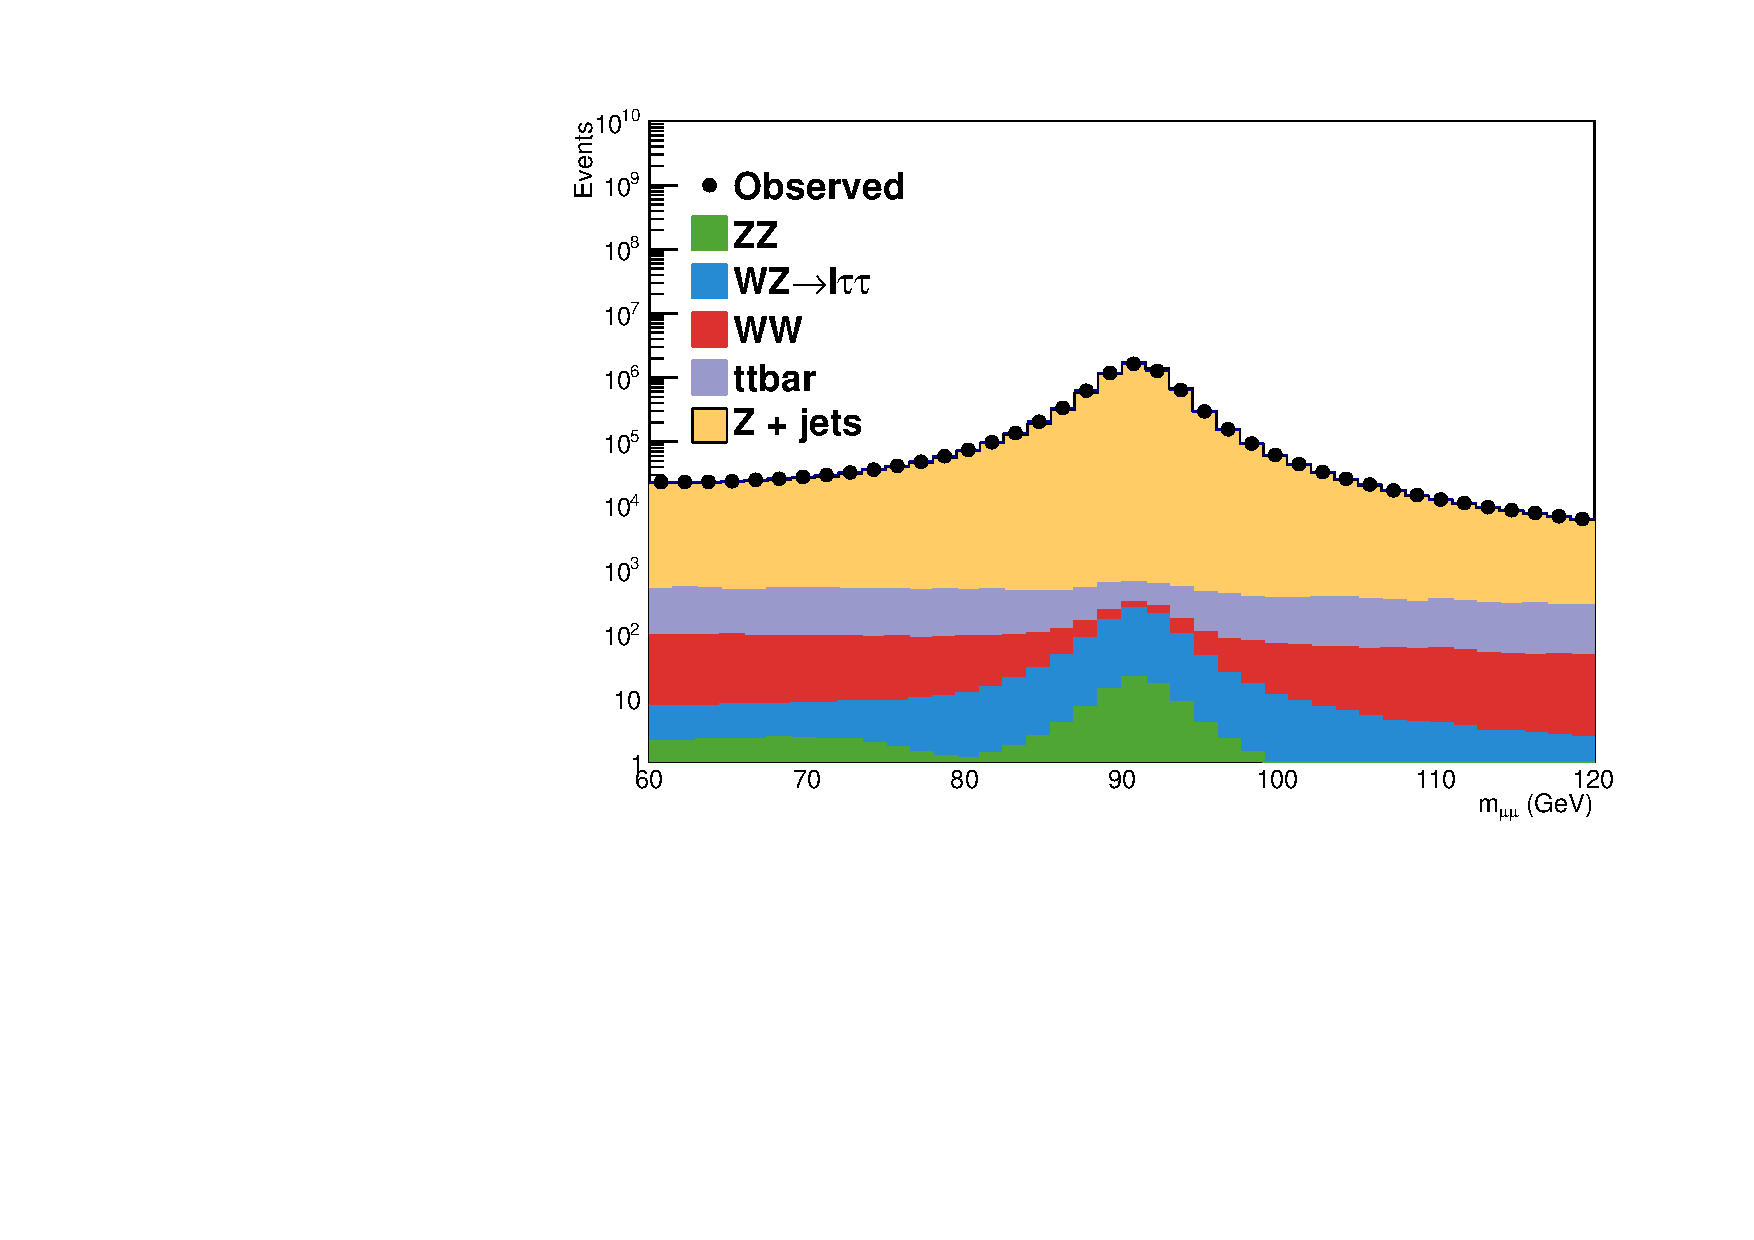
\includegraphics[width=0.49\textwidth]{4_Analisys/pics/8TeV/plots/zmm/mass_rebin_log.pdf}
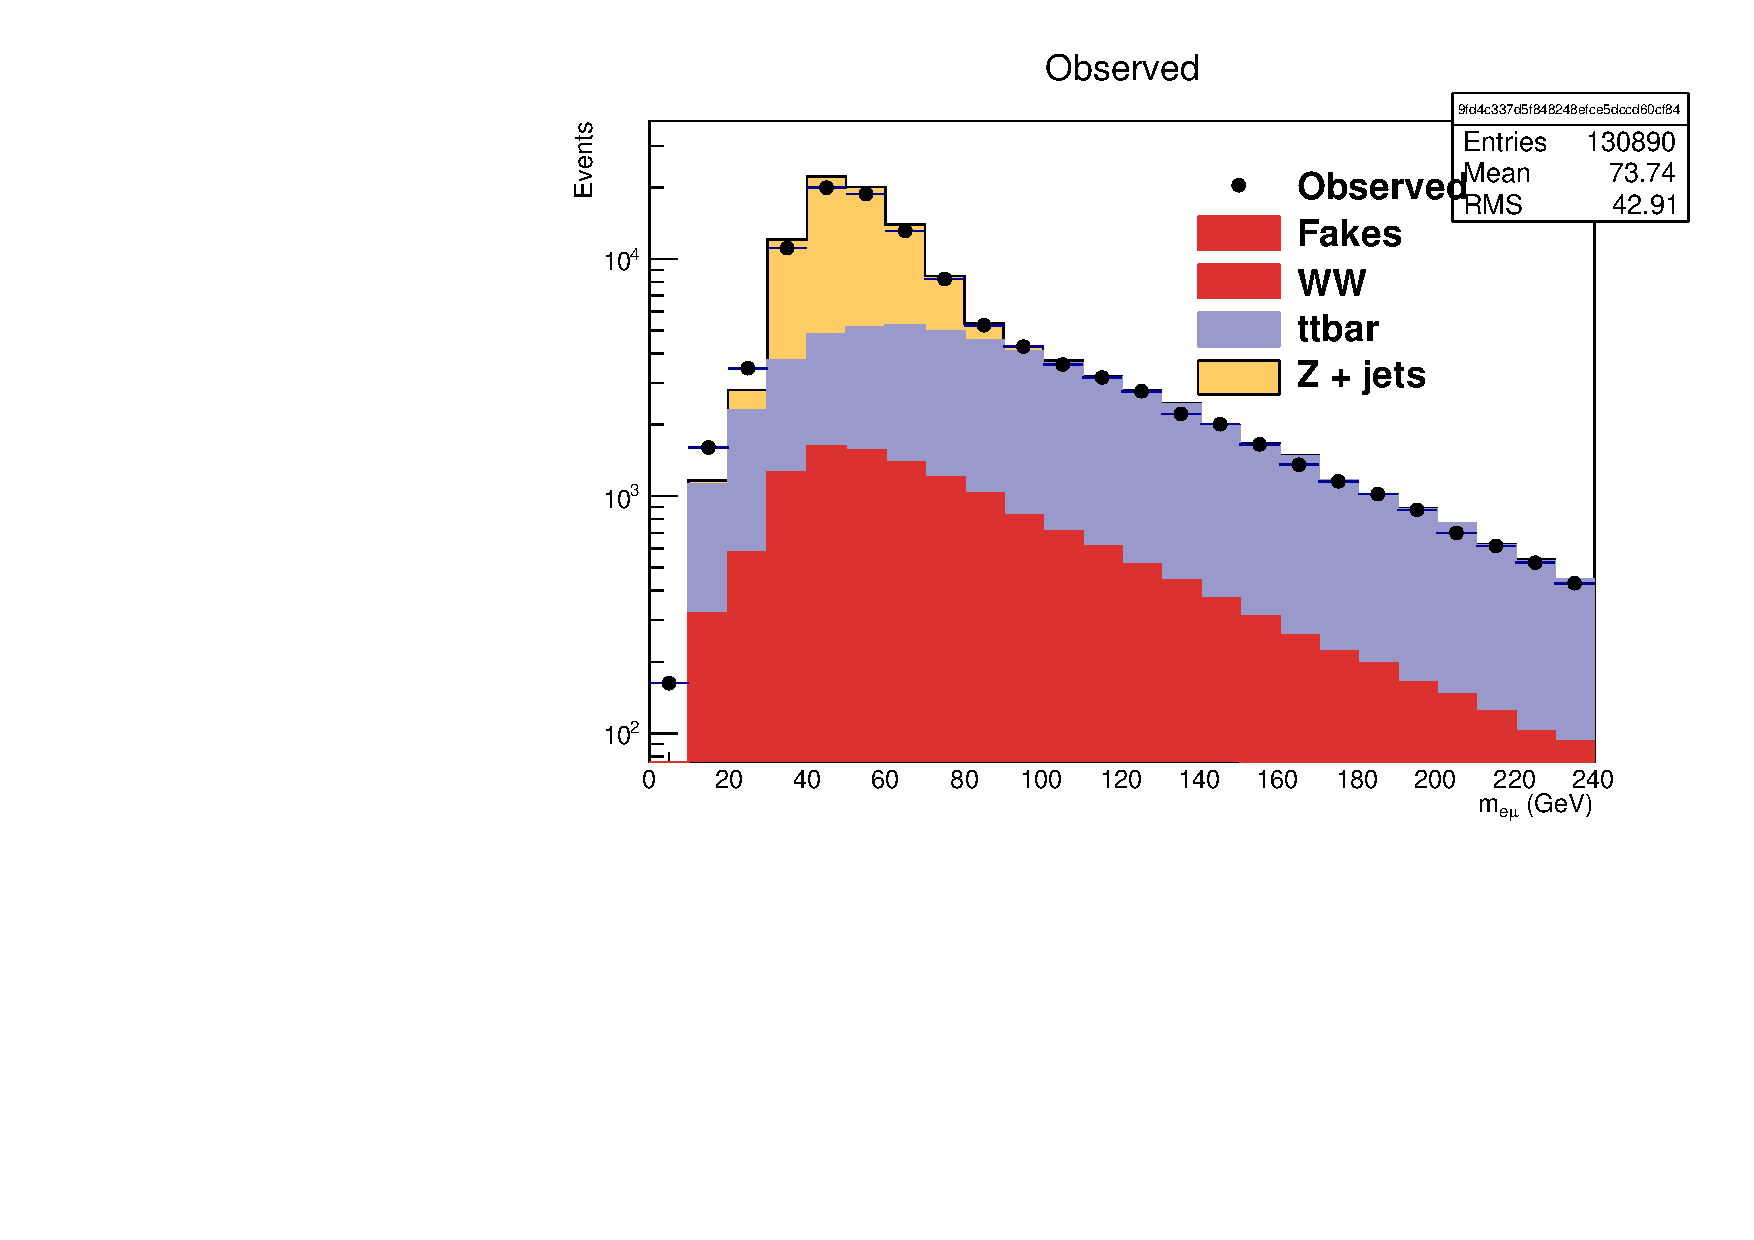
\includegraphics[width=0.49\textwidth]{4_Analisys/pics/8TeV/plots/em/mass_rebin_log-fakes.pdf}\\
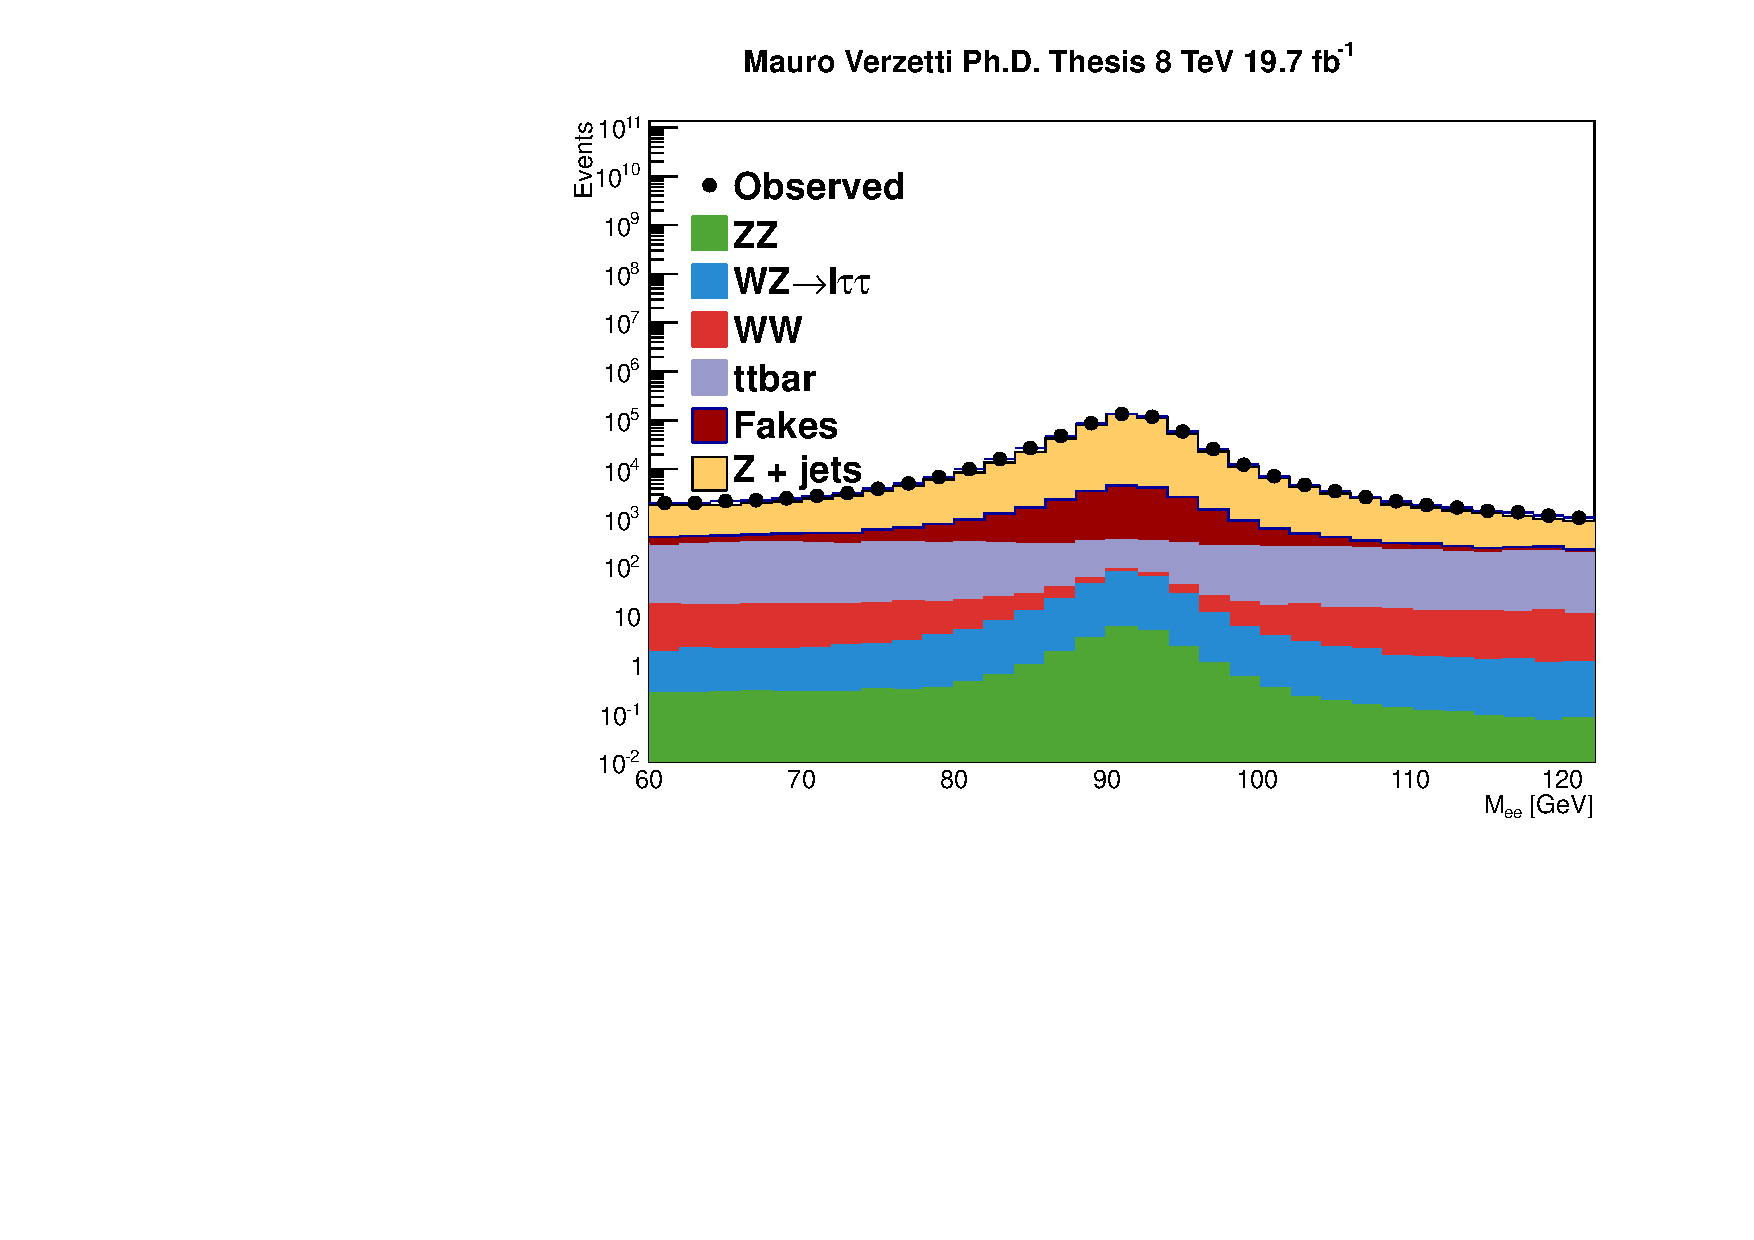
\includegraphics[width=0.49\textwidth]{4_Analisys/pics/8TeV/plots/zee/mass_wfakes_log.pdf}
\caption{Dilepton invariant mass distribution measured with 8 TeV data in dedicated $\Z\To\mu\mu$ (top left), $\Z\To \tau\tau \To e\mu$ (top right), and $\Z\To ee$ (bottom) control regions. Data are represented by solid points while the expectation is given by the stacked histogram. The background contributions labeled ``Fakes'' is estimated as described in Section~\ref{sec:fakemethod}. %are computed as the reducible background in the main analysis and described in the following section. 
}
\label{fig:(dis)agreement}
\end{figure}

\subsection{Reducible backgrounds}

The reducible background includes a wide range of processes with quark or gluon jets misidentified as leptons. %In these conditions a
A data-driven background estimation technique is preferred over simulation. %Due to these constraints 
In the work presented in this thesis the reducible backgrounds are estimated by means of the ``misidentification rate'' (or ``fake rate'') method.

The method consists of defining ``loose'' as well as ``tight'' selections for the lepton that can be faked by the jets, with the tight selection being the same as the final analysis selection used in this work.
The misidentification probability for a quark or gluon jet satisfying the loose lepton selections to pass the corresponding tight selection can be parametrized by a function $f(\vec{x})$ of a set of kinematic variables, $\vec{x}$, characterizing the event. This probability is measured in a dedicated control region resembling as closely as possible the signal region, while still being disjunct from it. The misidentification probability is then applied as weight to the events passing all selection criteria of the signal region except the tight lepton requirements. The weighted distributions obtained in this way represent the background contribution expected in the signal region.

%We study two possible background estimations: one using the $\rm{jet} \To \ell$ misidentification probability and the other using the $\rm{jet} \To \tau_h$ one. 
We compare the background estimates obtained by applying the method to the light leptons and to the tau leg. 
The former method is more inclusive as it accounts for all the sources of reducible backgrounds while the latter ignores those in which an isolated light lepton is mistakenly identified as an hadronic tau candidate. For these processes (i.e. Z+jets, WW, and part of $t\anti{t}$) the latter method relies on MC simulation. 

\subsection{Fake lepton method}
\label{sec:fakemethod}
\subsubsection{Control region definition}
The lepton misidentification probability is measured in a $W$+jets enriched control region.
This region differs from the signal one by requiring the transverse mass of the leading $\ell-\met$ system to exceed 55 GeV,
and vetoing events with more than two identified electron or muon candidates in the event. Events containing a well identified hadronic tau are vetoed as well, to remove any overlap with the signal region. In order to mimic the presence of a hadronic tau, the event is required to contain an additional jet with \pT above $20$ GeV.

Events selected in the control regions described above are used to train a k-Nearest Neighbor classifier (kNN)~\cite{TMVA}, which allows the parametrization of the misidentification probability as function of multiple variables. All the events selected in the control region are used to train the kNN.
Each parameter (dimension) is inversely scaled by its variance over the training sample, so that the (scaled) parameters are approximately normally distributed.
Those passing the tight lepton selection are marked as signal, those failing as background.
To find the misidentification probability at a particular point in the parameter space, the classifier searches for the $k$ nearest objects to the given point in the training sample.
The predicted efficiency is then the number of signal events among the $k$ neighbors and divided by $k$.
The input variable used for the training are the lepton \pT, the \pT of the jet associated to the lepton, and the number of jets with $\pt > 20$ GeV in the event. 
The first two variables, especially the jet \pT, are found to be strongly correlated to the probability for a jet to be mis-identified as a lepton. In particular, the difference of these two variables is linked to the isolation value of the lepton. In the training of the muon misidentification probabilities the logarithm of the jet \pT is used instead of the jet \pT to reduce the steep dependence of the probability with respect to this variable, allowing a larger number of neighbors to be used.
The number of jets was found to improve the description of the background shape. This variable is particularly effective in separating the different processes underlying the reducible background (W, multi-jet, and $t\anti{t}$). Another peculiarity of this variable is that it is bound to be $\geq 1$ in the training sample, while it can be zero in the main analysis. The difference is resolved by adding the number of hadronic taus in the event to the number of jets, resulting in a variable with the same range as the training variable.

The contribution of genuine isolated leptons from WZ and ZZ events in the control region is removed using simulated MC events and training dedicated kNN classifiers on them.
The output of the diboson kNN's is then scaled by:

\begin{equation}
\frac{N_{training}^{MC}}{N_{training}^{data}}\frac{\mathcal{L}^{data}}{\mathcal{L}_{eff}^{MC}}
\end{equation}

where $N_{training}^{i}$ is the number of events used for the training of either data or MC and $\mathcal{L}^{i}$ denotes the corresponding integrated luminosity. The output of the diboson kNN is finally subtracted to the output of the kNN trained on data.\footnote{Another equivalent option would have been to directly inject the simulated events in the training sample with negative weight proportional to the luminosity difference, but this method has been found to yield inconsistent results, most likely due to a wrong implementation in the TMVA framework.}

\subsubsection{kNN optimization and systematic uncertainties}
\label{sec:kNN_uncertainties}

The only adjustable parameter in the kNN training is the number of neighbors used to extract the probability. 
The optimal number of neighbors depends on the probability distribution of the different observables (more or less steeply varying) and of the statistics of the training sample. 
A large number of neighbors yields a very accurate results, at the price of a reduced ability to describe abrupt changes in the probability function.

It is therefore important to define a procedure that determines the optimal number of neighbors to be used for each sample as function of the tight working point employed in the final analysis. This evaluation is performed with a bootstrapping technique.
Each training sample is initially split into two sub--samples, one containing 90\% of the events and the other the remaining 10\%. In order to remove any bias due to the run period (different pileup conditions) the smaller dataset is evenly sampled from the full dataset. This procedure is repeated ten times to obtain a set of mutually exclusive pairs of ``large'' and ``small'' samples. Subsequently, a training of the kNN classifier is performed on each large sample and applied to the small one. This procedure ensure a total decoupling between testing and training samples. The small size difference between the large sample and the full dataset also ensures that the results inferred from the major dataset are still statistically valid for the full one. The outcome of the ten training and testing cycles is then combined. 

The full process is repeated to scan over a wide range of values for the number of neighbors, k. A strong limiting factor for this method is the significant computing resource usage, as the computing complexity of training and testing of the kNN algorithm is proportional to the number of neighbors used.% The choice of the tested points and their maximum value are a direct consequence of this limitation: as the number of neighbors increases, the scan becomes more coarse.

For each choice of k, the shape of important physics observables is computed based on the weighted sum of all the events in the small samples and from the passing events. The two shapes are compared using as figure of merit the $\chi^2$ compatibility between the two shapes. The physical observable used for the $\chi^2$ minimization is the scalar sum of the \pT of the two leptons plus the jet, similar to the $L_T$ variable used further on in the analysis. Other variables were also considered and found to yield similar conclusions concerning the optimal choice of k.%compatible results. 

The minimum $\chi^2$ value obtained by the scan is taken to define k for training the final kNN algorithm used in the analysis.%as reference value of number of neighbors to be used for training in the analysis. 
A parabolic fit around the minimum is performed to estimate the one sigma confidence interval as the value for which the parabolic fit yields the value of $\chi^2_{min} + 1$. %is $fcn(i) = \chi^2_{min} + 1$. 
This confidence interval reflects both the statistical uncertainties on the training sample and the related uncertainty on the choice of the parameters. For each channel and each lepton, three classifiers are trained with the corresponding central values and one sigma boundaries.

A summary of the chosen minima and of the confidence interval boundaries is given in table \ref{tab:kNN_minima}. A graphic representation of a sample scan is shown in figure \ref{fig:kNN_minima_sample}. The misidentification rate observed in the training sample is displayed in figure \ref{fig:fake_rate_sample}, overlaid with the output of the respective kNN classifier.


\begin{table}

\caption{Minimization points for each kNN scan and relative uncertainties as obtained from a parabolic fit}

\centering
\begin{tabular}{|c|c|c|c|c|}
\hline
channel & lepton & $-1\,\sigma$ & central value & $1\,\sigma$ \\
\hline
\multicolumn{5}{|c|}{7 TeV} \\
\hline
\multirow{2}{*}{ $\mu\mu\tau_h$ }& leading muon & 15 & 20 & 60\\
& sub-leading muon & 11 & 20 & 49\\
\hline
\multirow{2}{*}{ $e\mu\tau_h$ }& muon & 7 & 20 & 30\\
& electron & 634 & 1000 & 1807\\
\hline
\multirow{2}{*}{ $ee\tau_h$ }& leading electron & 35 & 200 & 686\\
& sub-leading electron & 381 & 1200 & 1723\\
\hline
\multicolumn{5}{|c|}{8 TeV} \\
\hline
\multirow{2}{*}{ $\mu\mu\tau_h$ }& leading muon & 28 & 40 & 73\\
& sub-leading muon & 30 & 40 & 63\\
\hline
\multirow{2}{*}{ $e\mu\tau_h$ }& muon & 16 & 20 & 30\\
& electron & 664 & 1400 & 2136\\
\hline
\multirow{2}{*}{ $ee\tau_h$ }& leading electron & 218 & 400 & 552\\
& sub-leading electron & 605 & 1000 & 2201\\
\hline
\end{tabular}

\label{tab:kNN_minima}
\end{table}

\begin{figure}
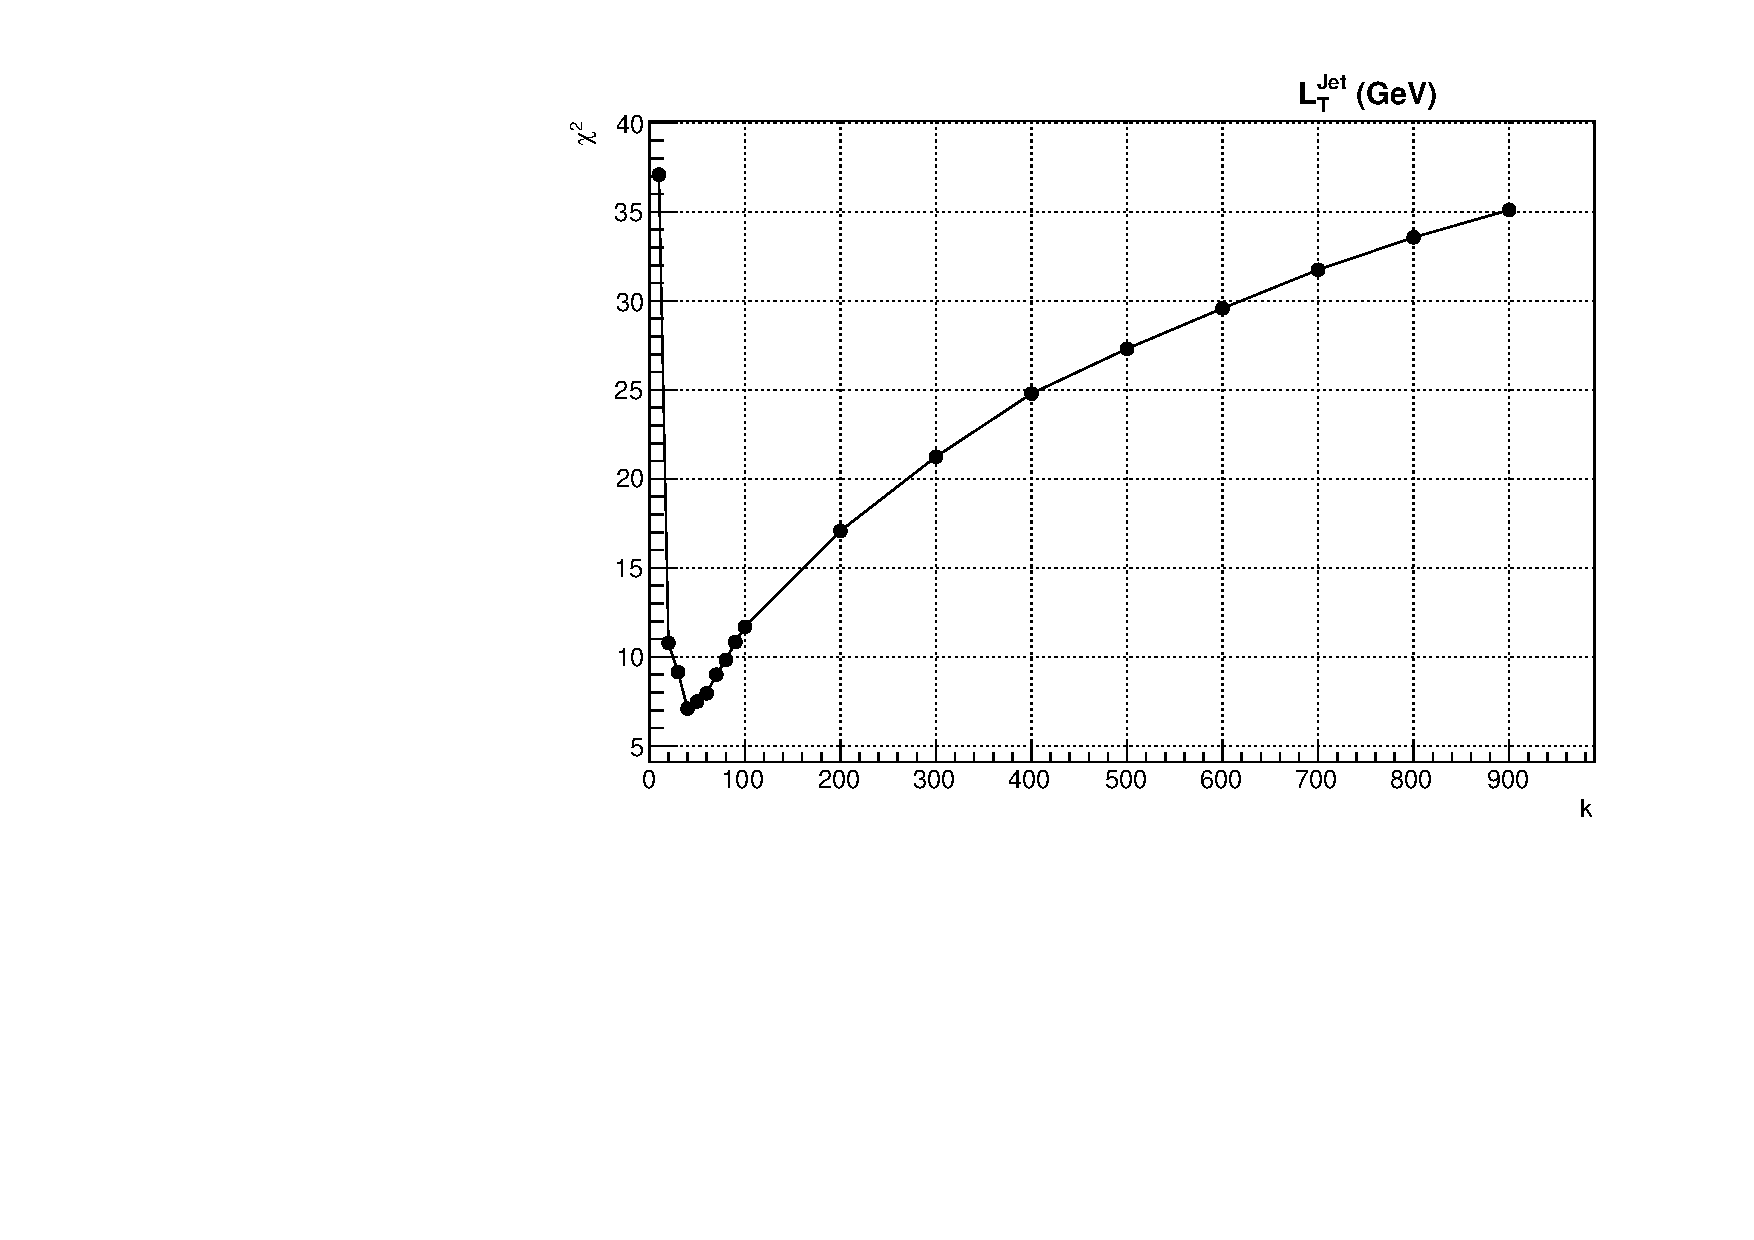
\includegraphics[width=0.5\textwidth]{4_Analisys/pics/8TeV/ProfileNeighbors/MM/h2taucuts020/LT_chi2.pdf}
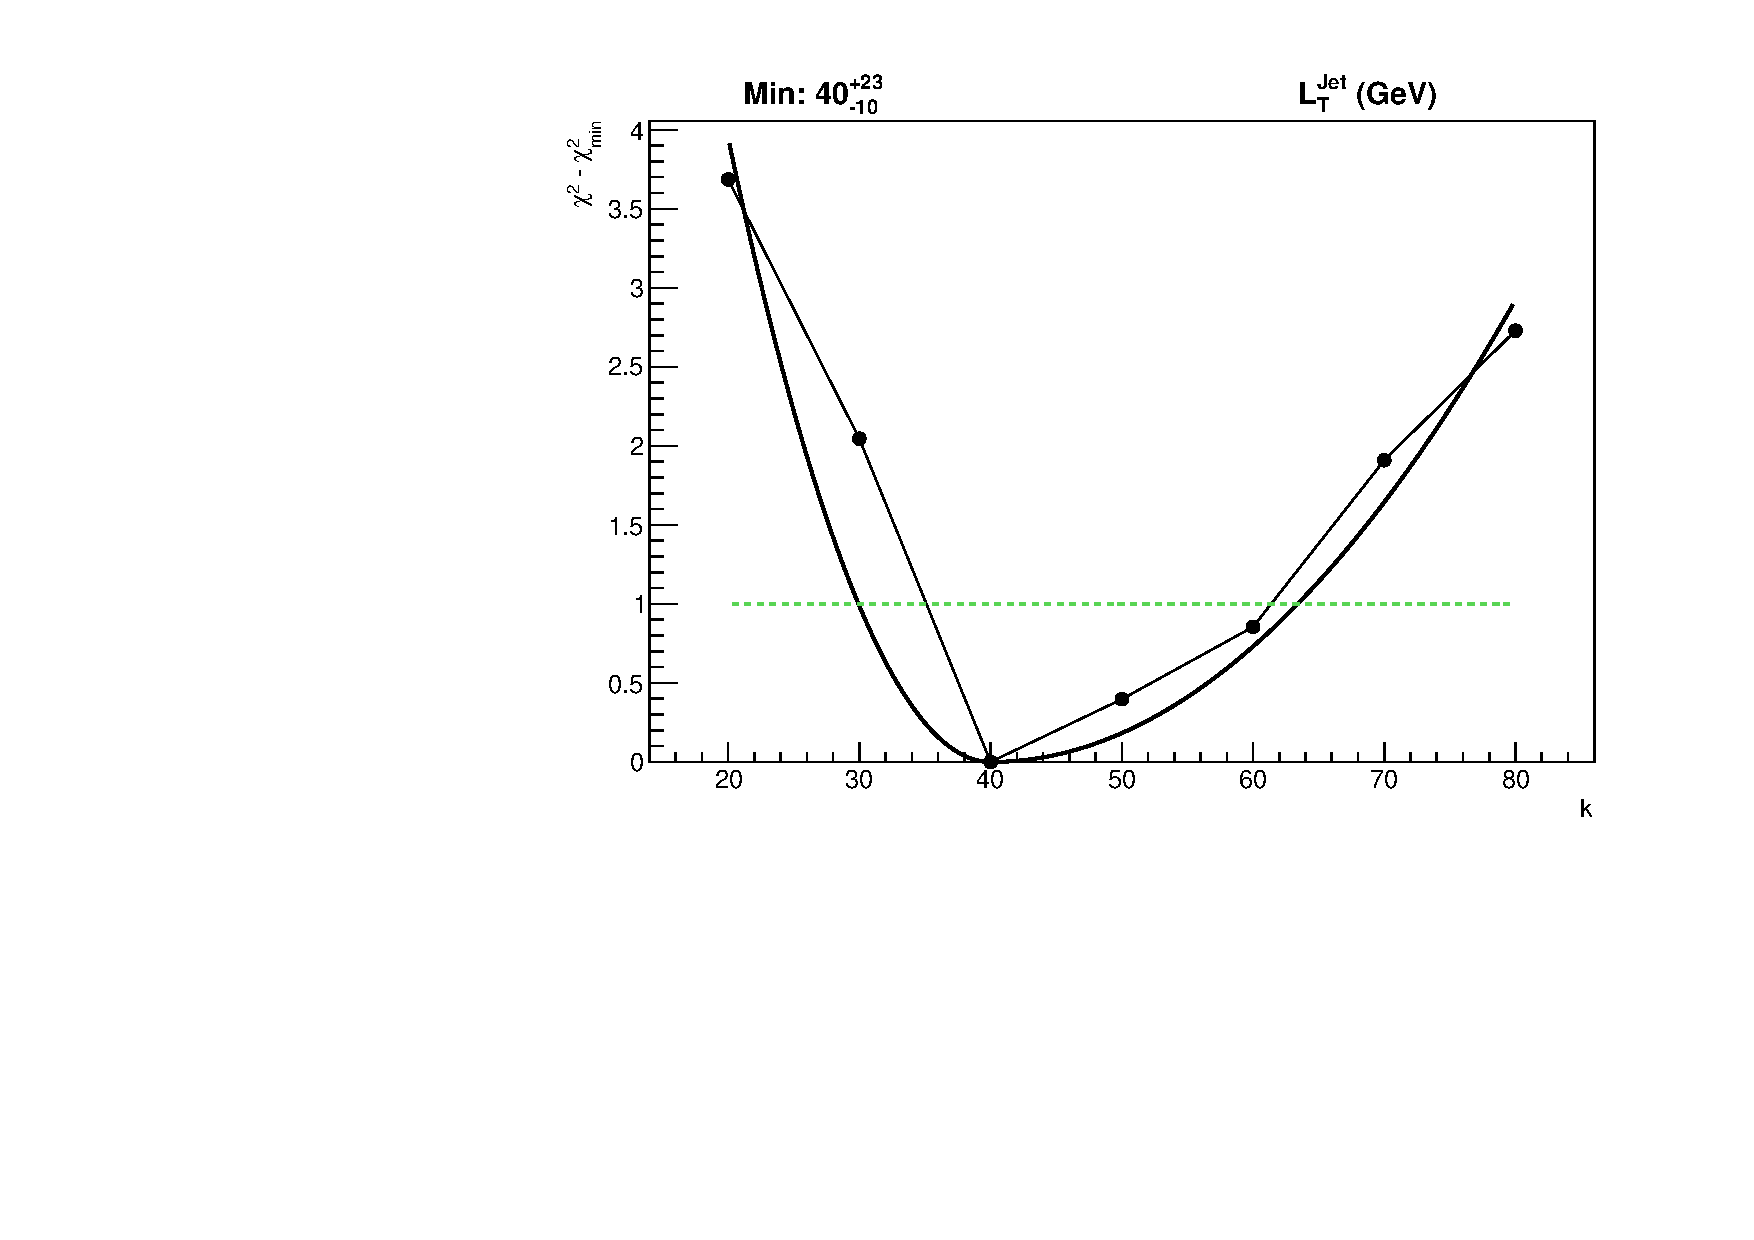
\includegraphics[width=0.5\textwidth]{4_Analisys/pics/8TeV/ProfileNeighbors/MM/h2taucuts020_LT.pdf} \\
\caption{\chisq as a function of the number of neighbors used in the kNN algorithm for background estimation 
(left) and corresponding fit (right) for sub-leading muons in the $\mu\mu\tau_h$ channel. The variable used for the scan is the scalar sum of the \pT of the two leptons and the jet}
\label{fig:kNN_minima_sample}
\end{figure}

\begin{figure}
\centering
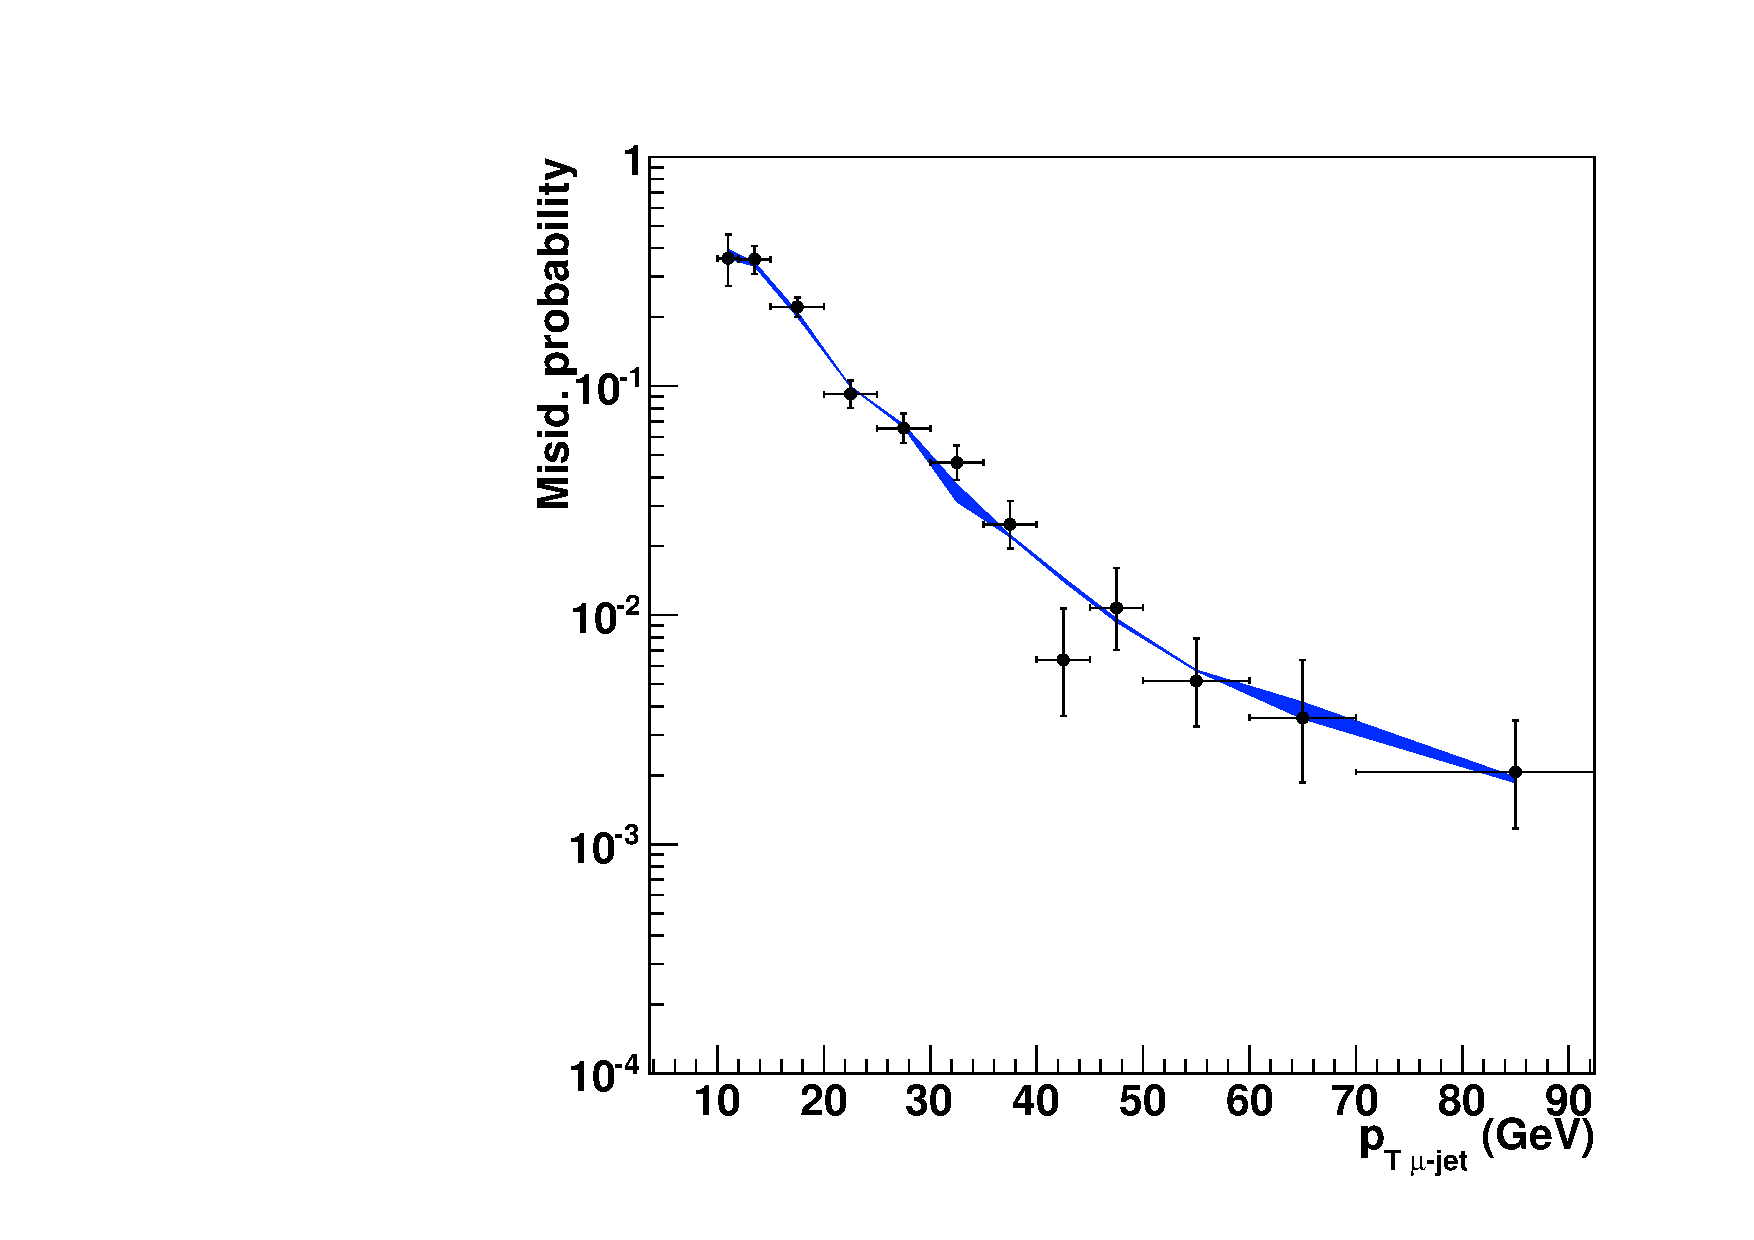
\includegraphics[width=0.49\textwidth]{4_Analisys/pics/8TeV/plots/fakerates/m_mmt_subleading_kNN_muonJetPt.pdf}
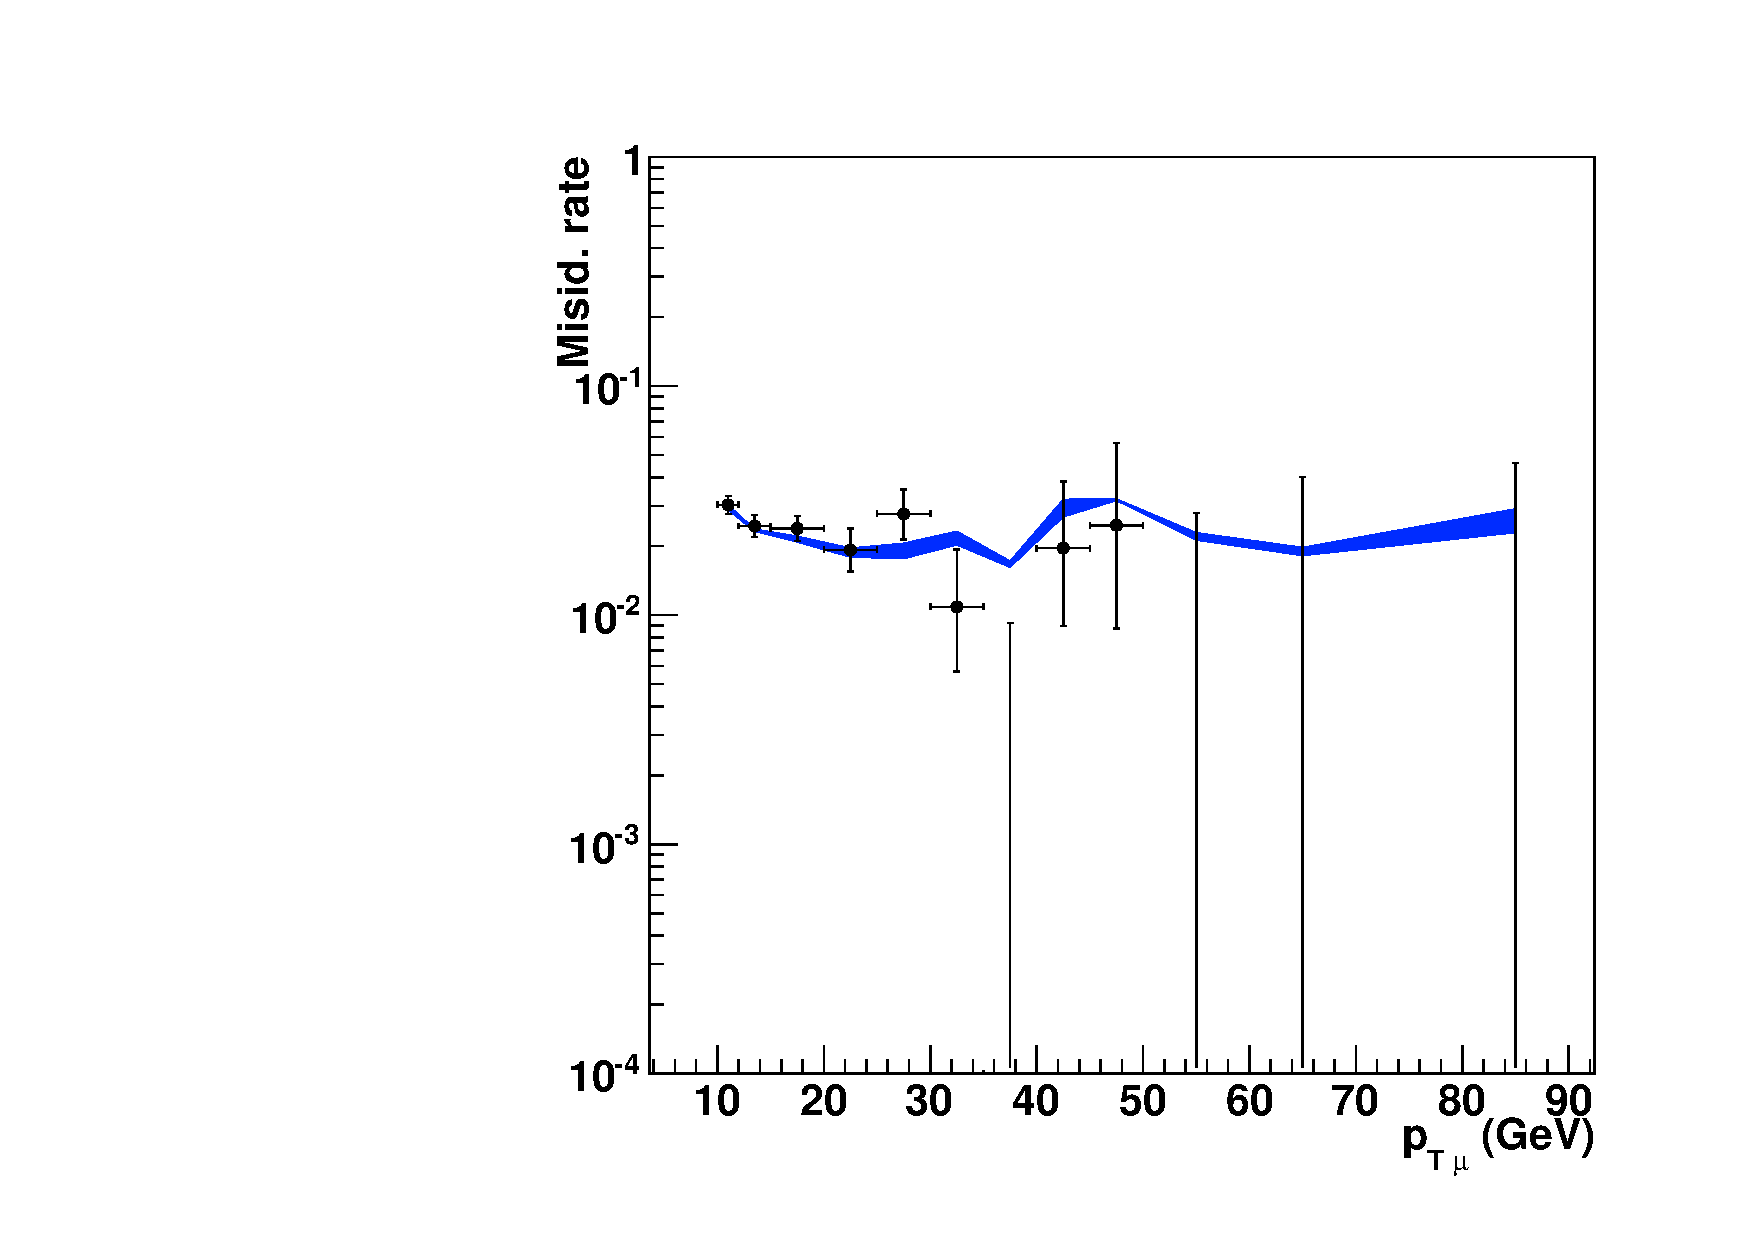
\includegraphics[width=0.49\textwidth]{4_Analisys/pics/8TeV/plots/fakerates/m_mmt_subleading_kNN_muonPt.pdf}\\
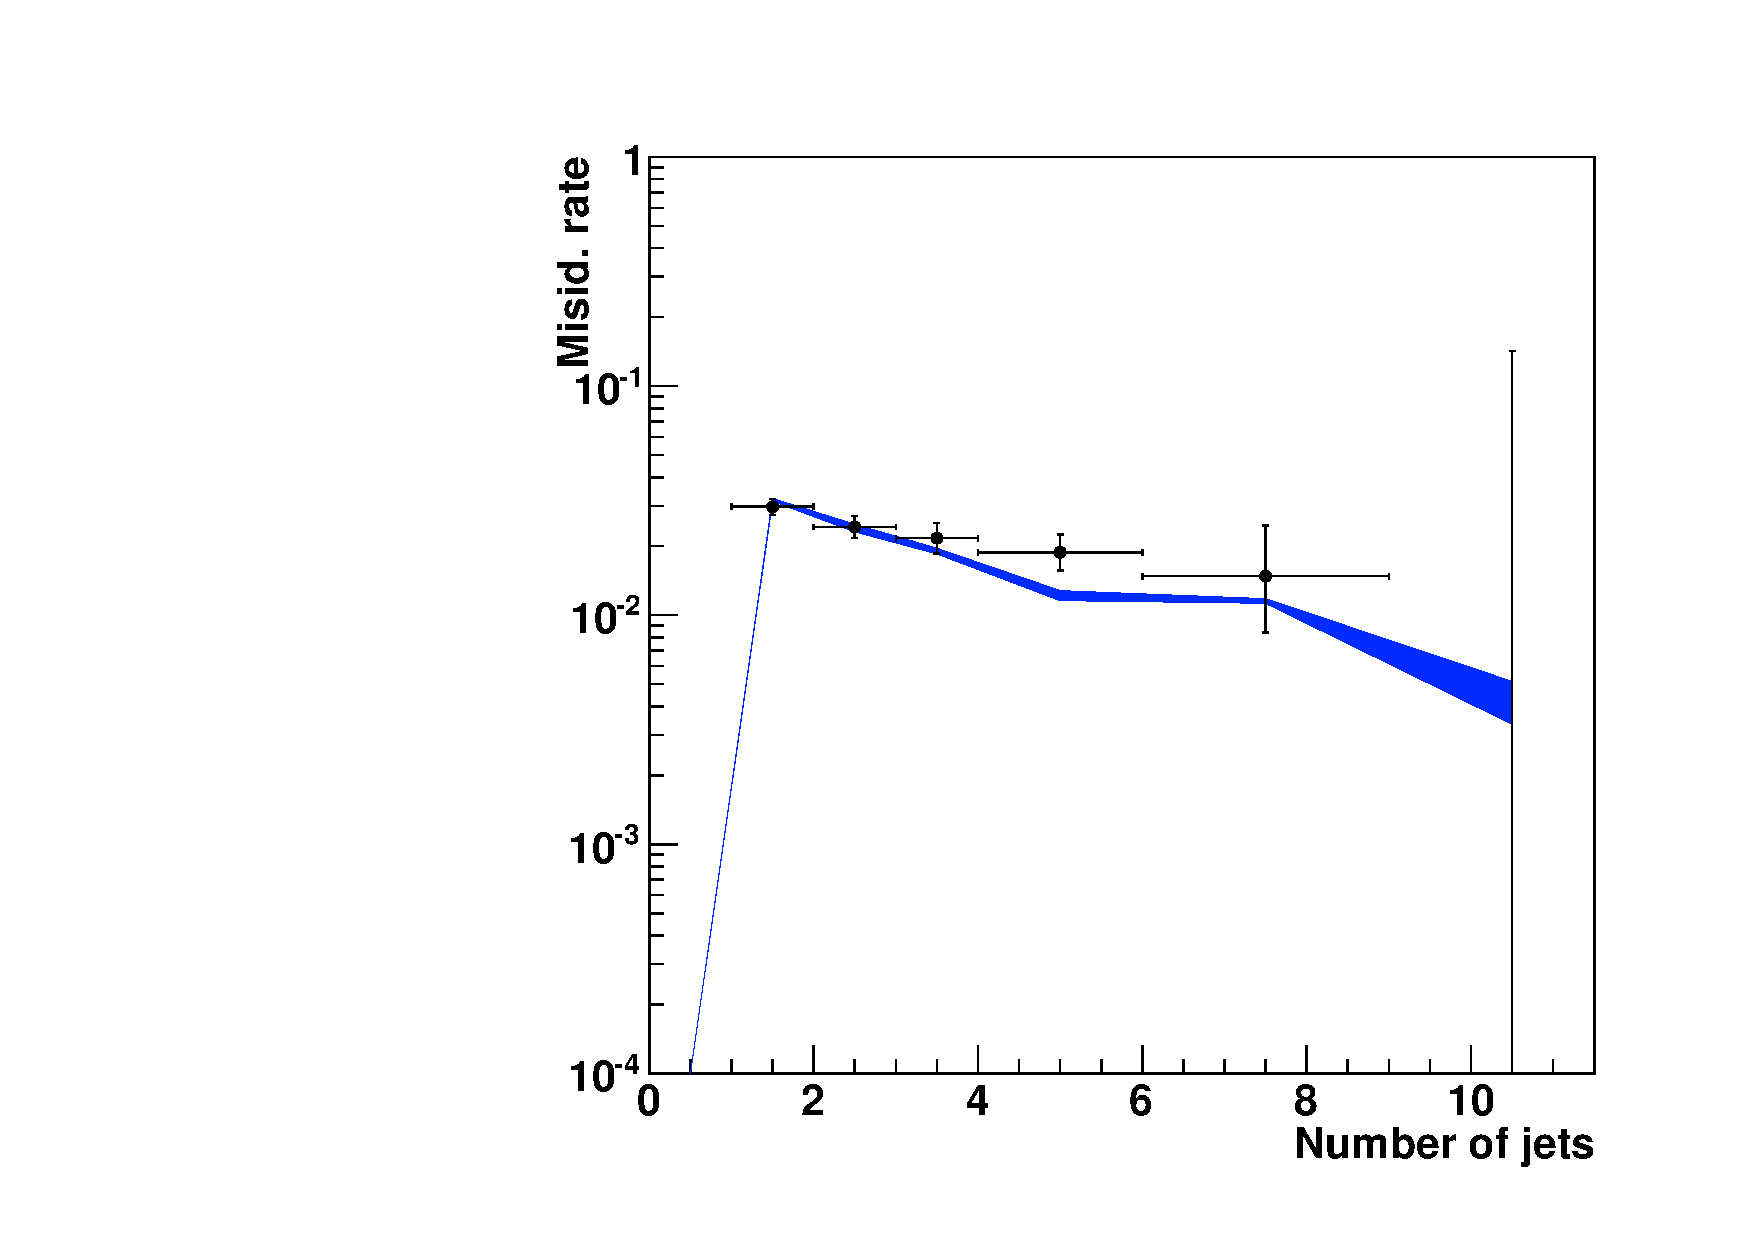
\includegraphics[width=0.49\textwidth]{4_Analisys/pics/8TeV/plots/fakerates/m_mmt_subleading_kNN_numJets20.pdf}
\caption{Measured misidentification probability for sub-leading muons in the training sample dedicated to the $\mu\mu\tau_h$ channel. The blue band represents the output of the kNN algorithm and its related uncertainty.}
\label{fig:fake_rate_sample}
\end{figure}


\subsubsection{Background shape extraction}
The contribution to the signal region from backgrounds containing a given fake object is estimated using an ``anti-isolated'' sideband in which the loose, but \emph{not} the tight, 
selection requirement is satisfied for that object. Events can therefore be divided into three categories:

\begin{enumerate}
\item Events in which the first lepton fails the tight requirements are weighted by $w_1(\vec{x}) = f_1(\vec{x})/(1-f_1(\vec{x}))$
\item Events in which the second lepton fails the tight requirements are weighted by $w_2(\vec{x}) = f_2(\vec{x})/(1-f_2(\vec{x}))$
\item Events in which the both lepton fail the tight requirements are weighted by $w_1(\vec{x}) \cdot w_2(\vec{x})$
\end{enumerate}

Each weighted category represents the contribution to the signal region of the backgrounds in which jets fake one or both the light leptons. As the events 
in which both reconstructed leptons are due to $\rm{jet}\To\ell$ fakes %where jets are mis-reconstructed as both leptons 
are included in category 1 as well as in category 2, it is necessary to remove the double-counting by subtracting the weighted events of category three, obtaining:

\begin{equation}
N_{bkg} = N_1 + N_2 - N_3
\end{equation}

where $N_{bkg}$ denotes the final estimate for the number of background events in the signal region and $N_i$ denotes the scaled number events in category $i$.

%Sys uncertainty
Uncertainties on the kNN training, evaluated as described above, are propagated to the background estimate for the signal region by comparing %computing 
the event weights obtained with classifiers trained with the central value and with the two one-sigma boundaries. The difference is taken as systematic uncertainty.

%Empty bins
In rare cases, especially in the tail of kinematic distributions, statistical fluctuations cause the number of weighted events in category three to exceed the sum of $N_1 + N_2$, %the other two categories, 
and therefore the expected yield in the signal region becomes negative. In these cases the yield is set to the value of category three only, relying on the much larger statistics present in that sideband.


%

\subsection{Validation of the fake lepton method}
\label{sec:f3_validation}

The method for estimating the reducible backgrounds is validated in two control regions which are dominated by fake $\tau_h$ candidates.
%This exercises all mechanisms of the reducible background estimation, since the $\tau_h$ candidate never participates in the misidentification rate method.
These control regions provide an independent validation, as they are naturally exclusive with respect to the event sample used to train the kNN. Events in the control region are selected by maintaining
the light-lepton same-charge requirement, but inverting the isolation requirement of the $\tau_h$ candidate and in one of the regions the charge of the tau is furthermore required to be the same as the leptons.
This regions are dominated by W+jets and $t\anti{t}$ backgrounds.
Comparison between the observed and predicted kinematic distributions in the control regions is shown for the $\mu\mu\tau_h$, $e\mu\tau_h$ and $ee\tau_h$ channels in figures~\ref{fig:LLT_mmt_f3_control_7TeV}--\ref{fig:LLT_eet_f3_control_8TeV} respectively.
Reasonable agreement is observed, considering that the expected background in this region lacks an additional systematic uncertainty, described in the next section and not defined in this region, which has sizable effect both on the distribution and total normalization of the fake background.

\begin{figure}
\begin{center}
  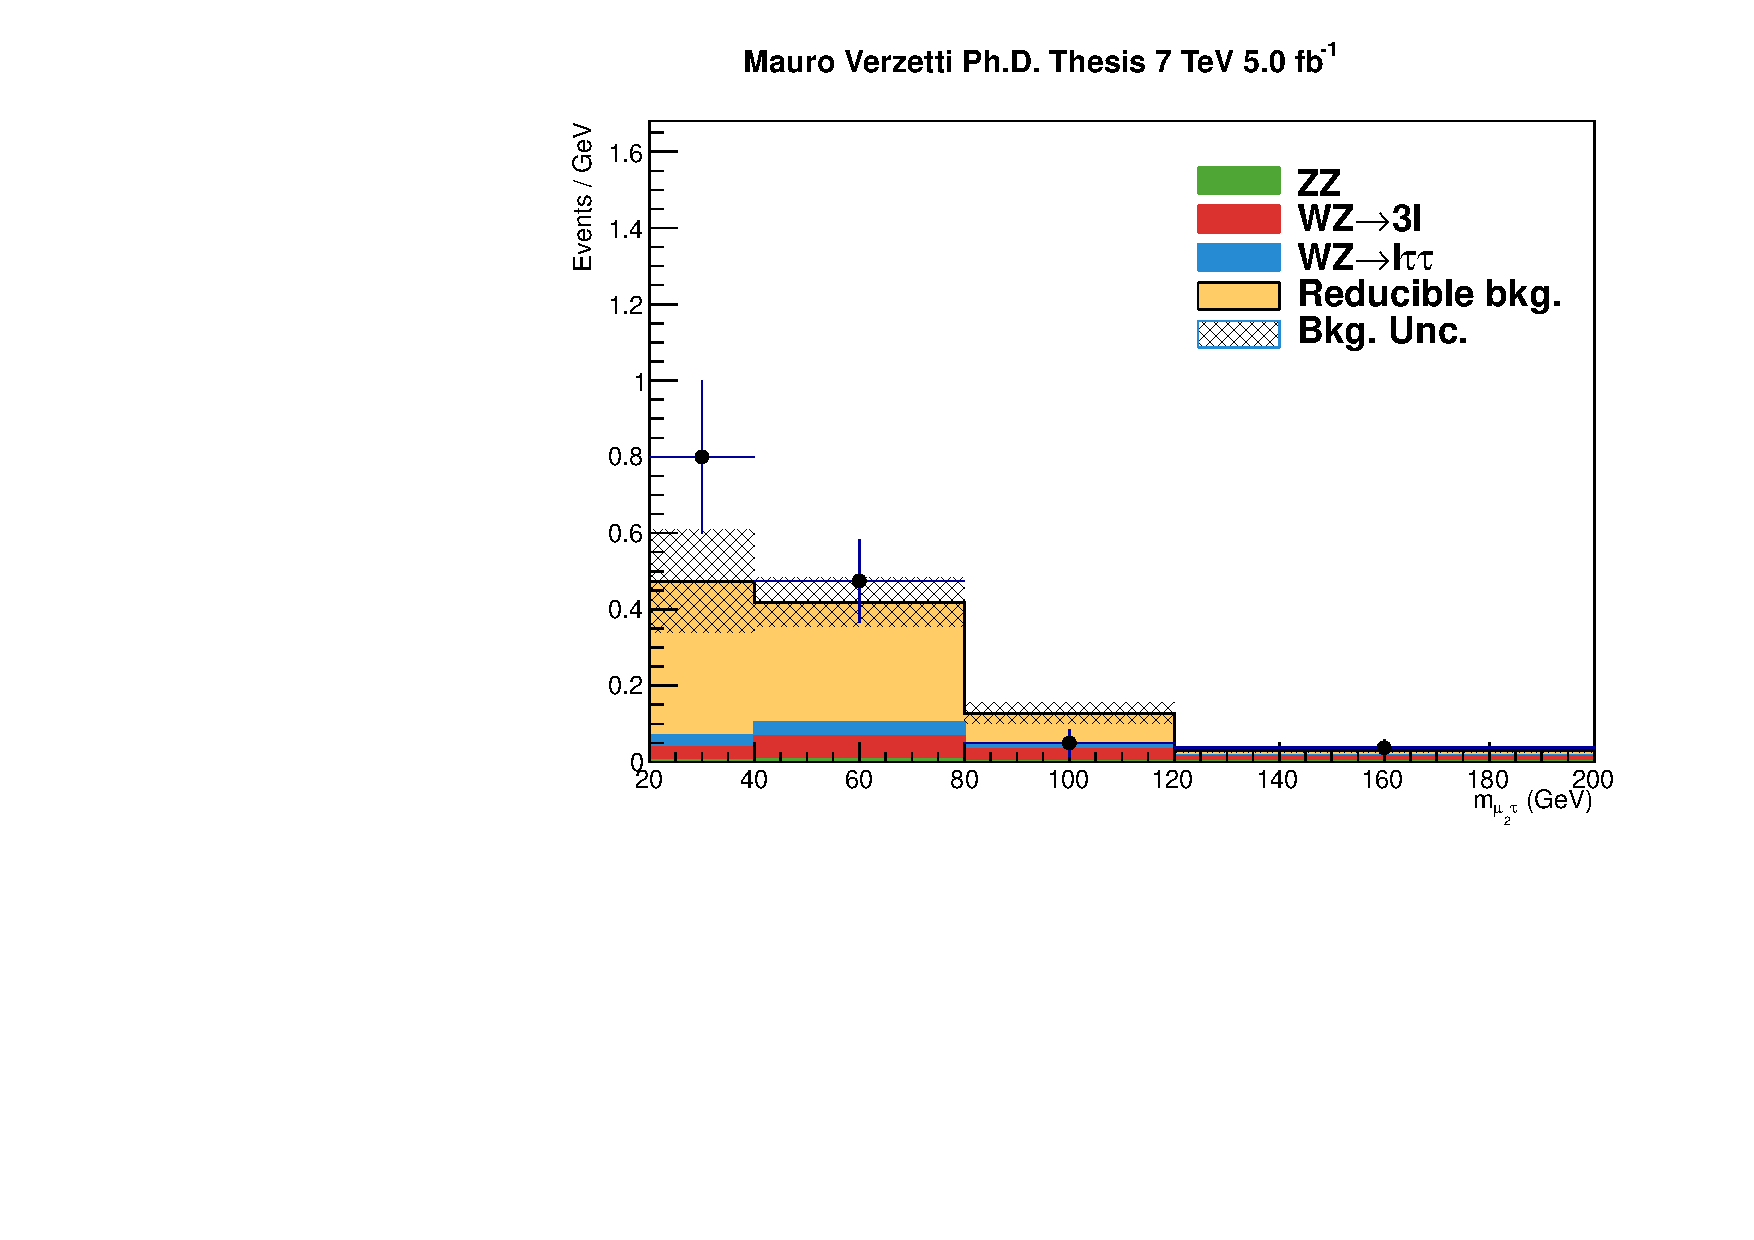
\includegraphics[width=0.49\textwidth]{4_Analisys/pics/7TeV/plots/mmt/f3/Full/final-f3-subMass-Full.pdf}
  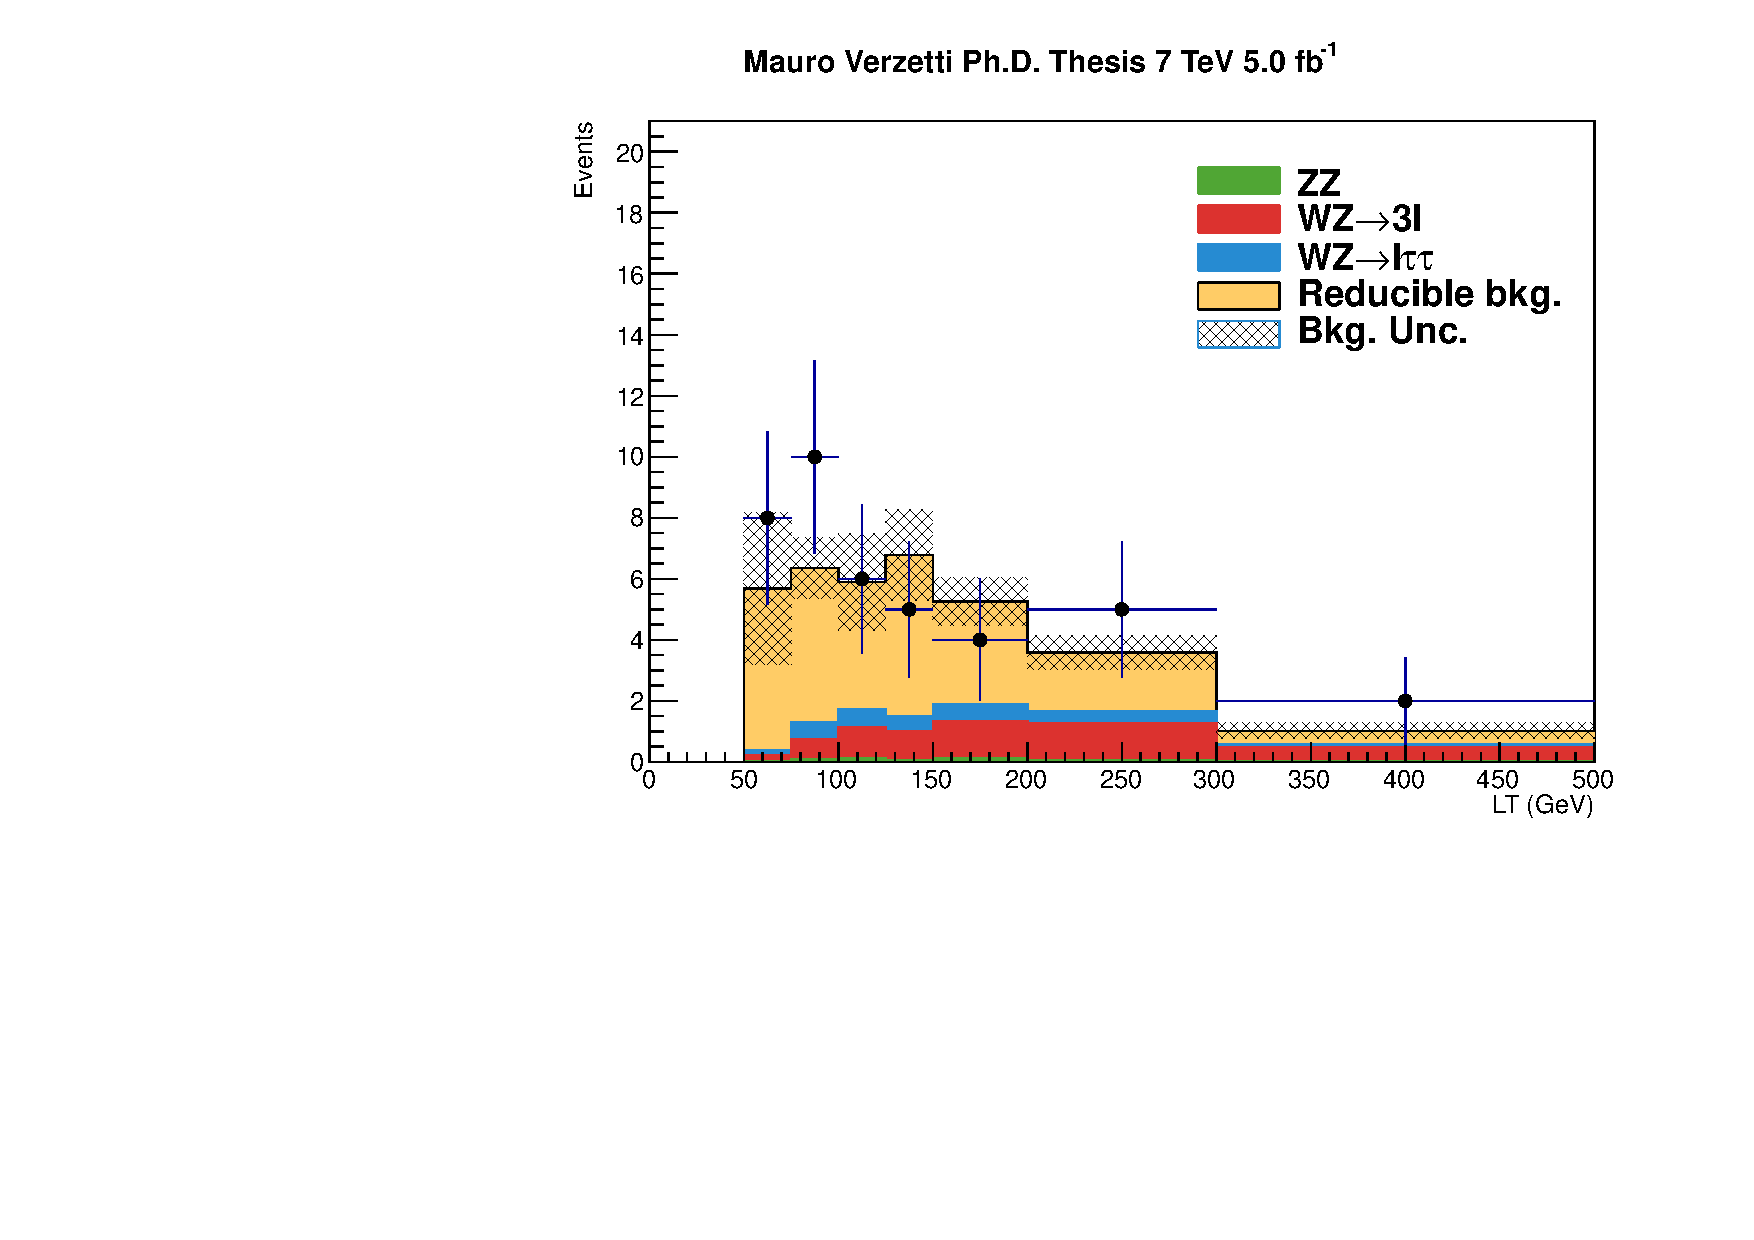
\includegraphics[width=0.49\textwidth]{4_Analisys/pics/7TeV/plots/mmt/f3/final-LT.pdf}\\
  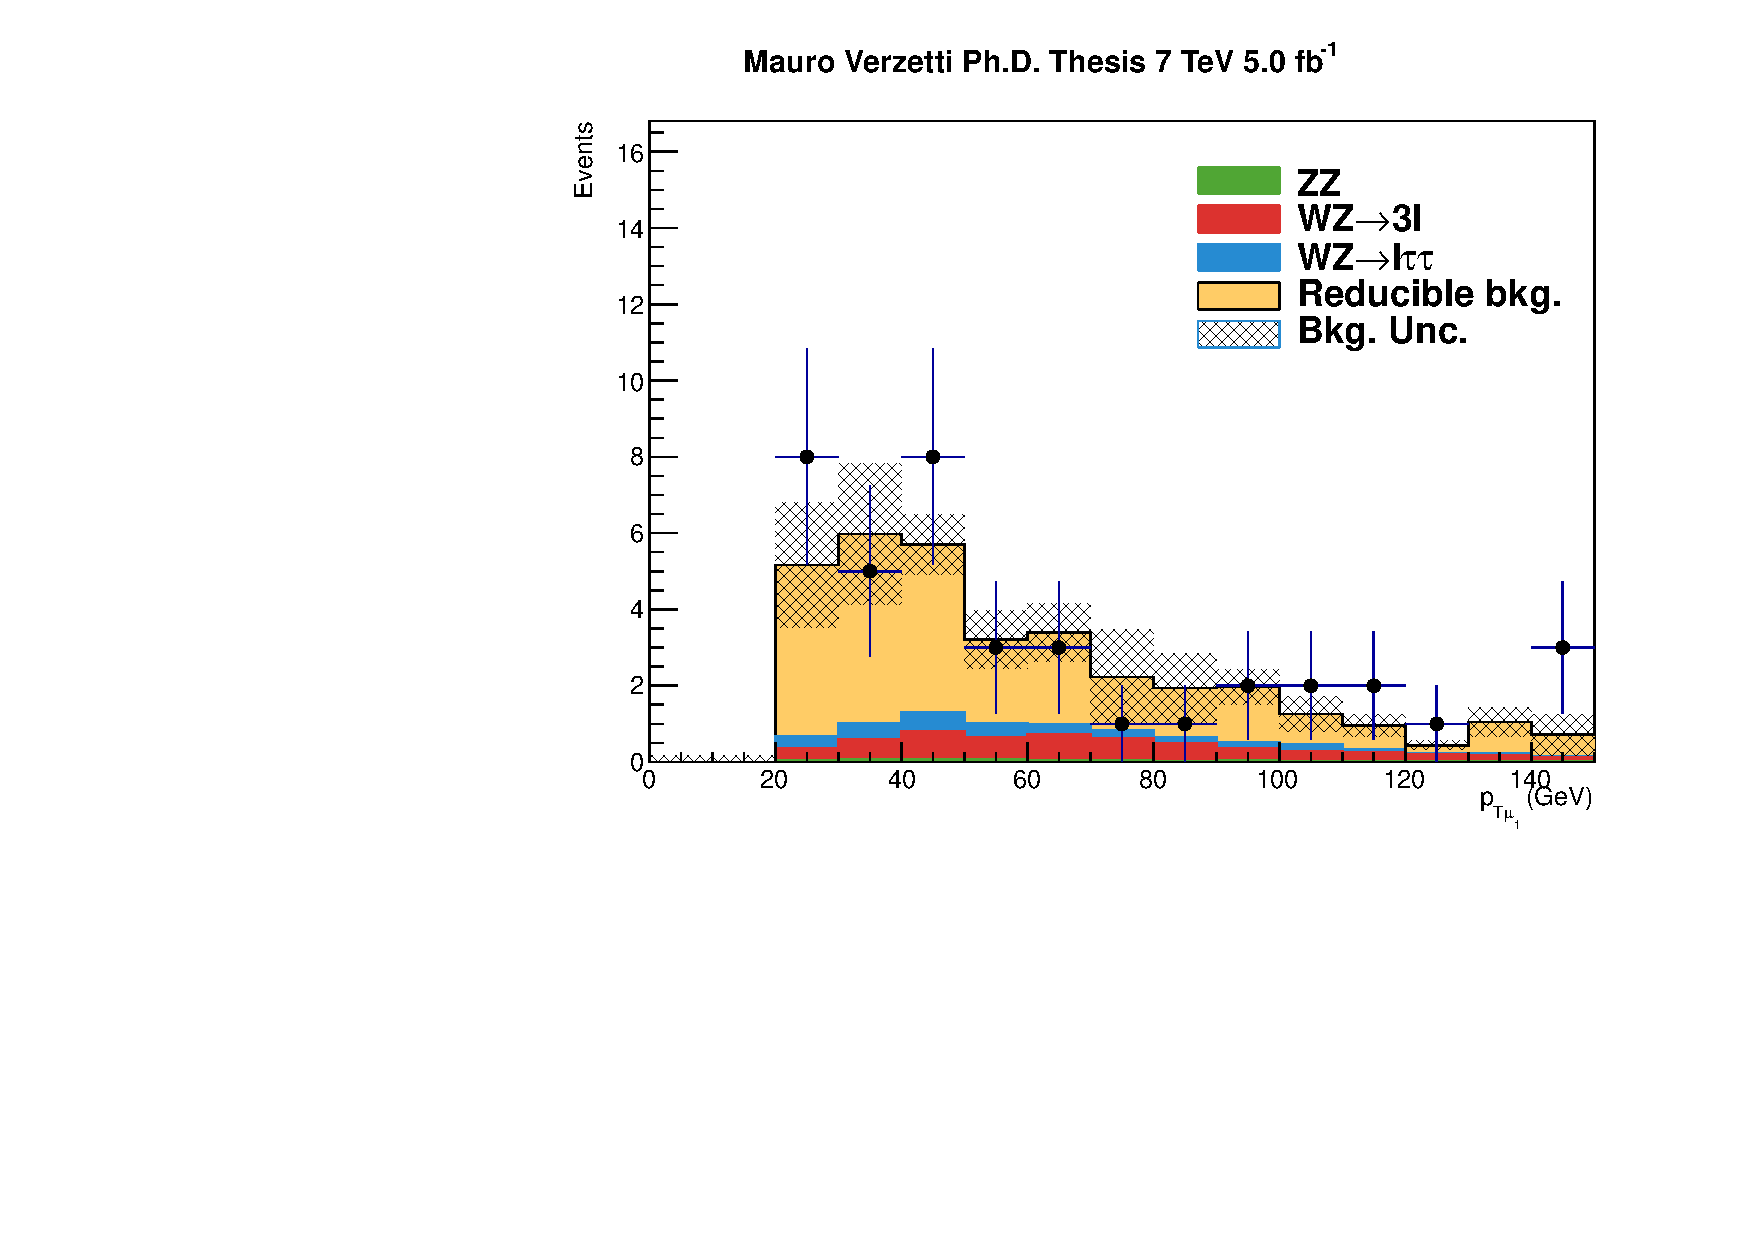
\includegraphics[width=0.49\textwidth]{4_Analisys/pics/7TeV/plots/mmt/f3/Full/final-f3-m1Pt-Full.pdf}
  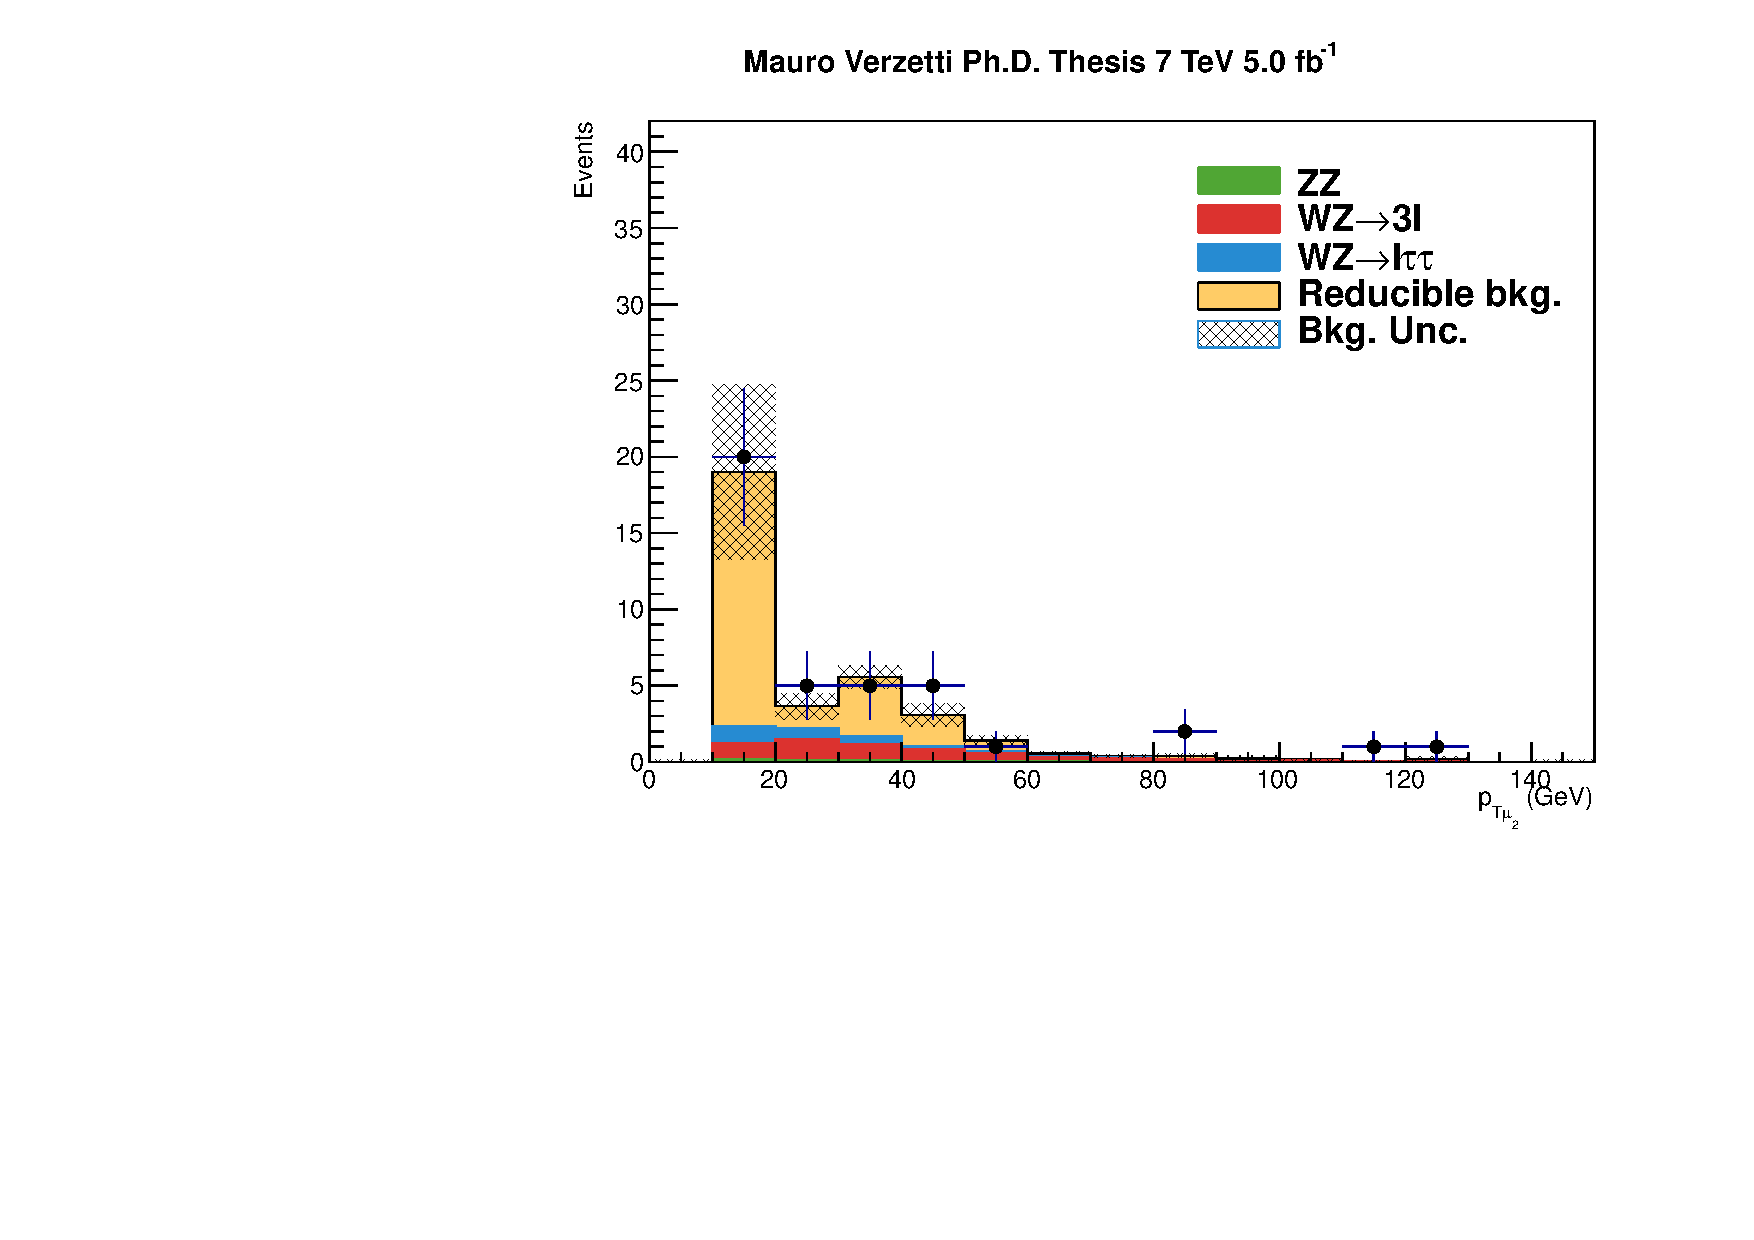
\includegraphics[width=0.49\textwidth]{4_Analisys/pics/7TeV/plots/mmt/f3/Full/final-f3-m2Pt-Full.pdf}\\
  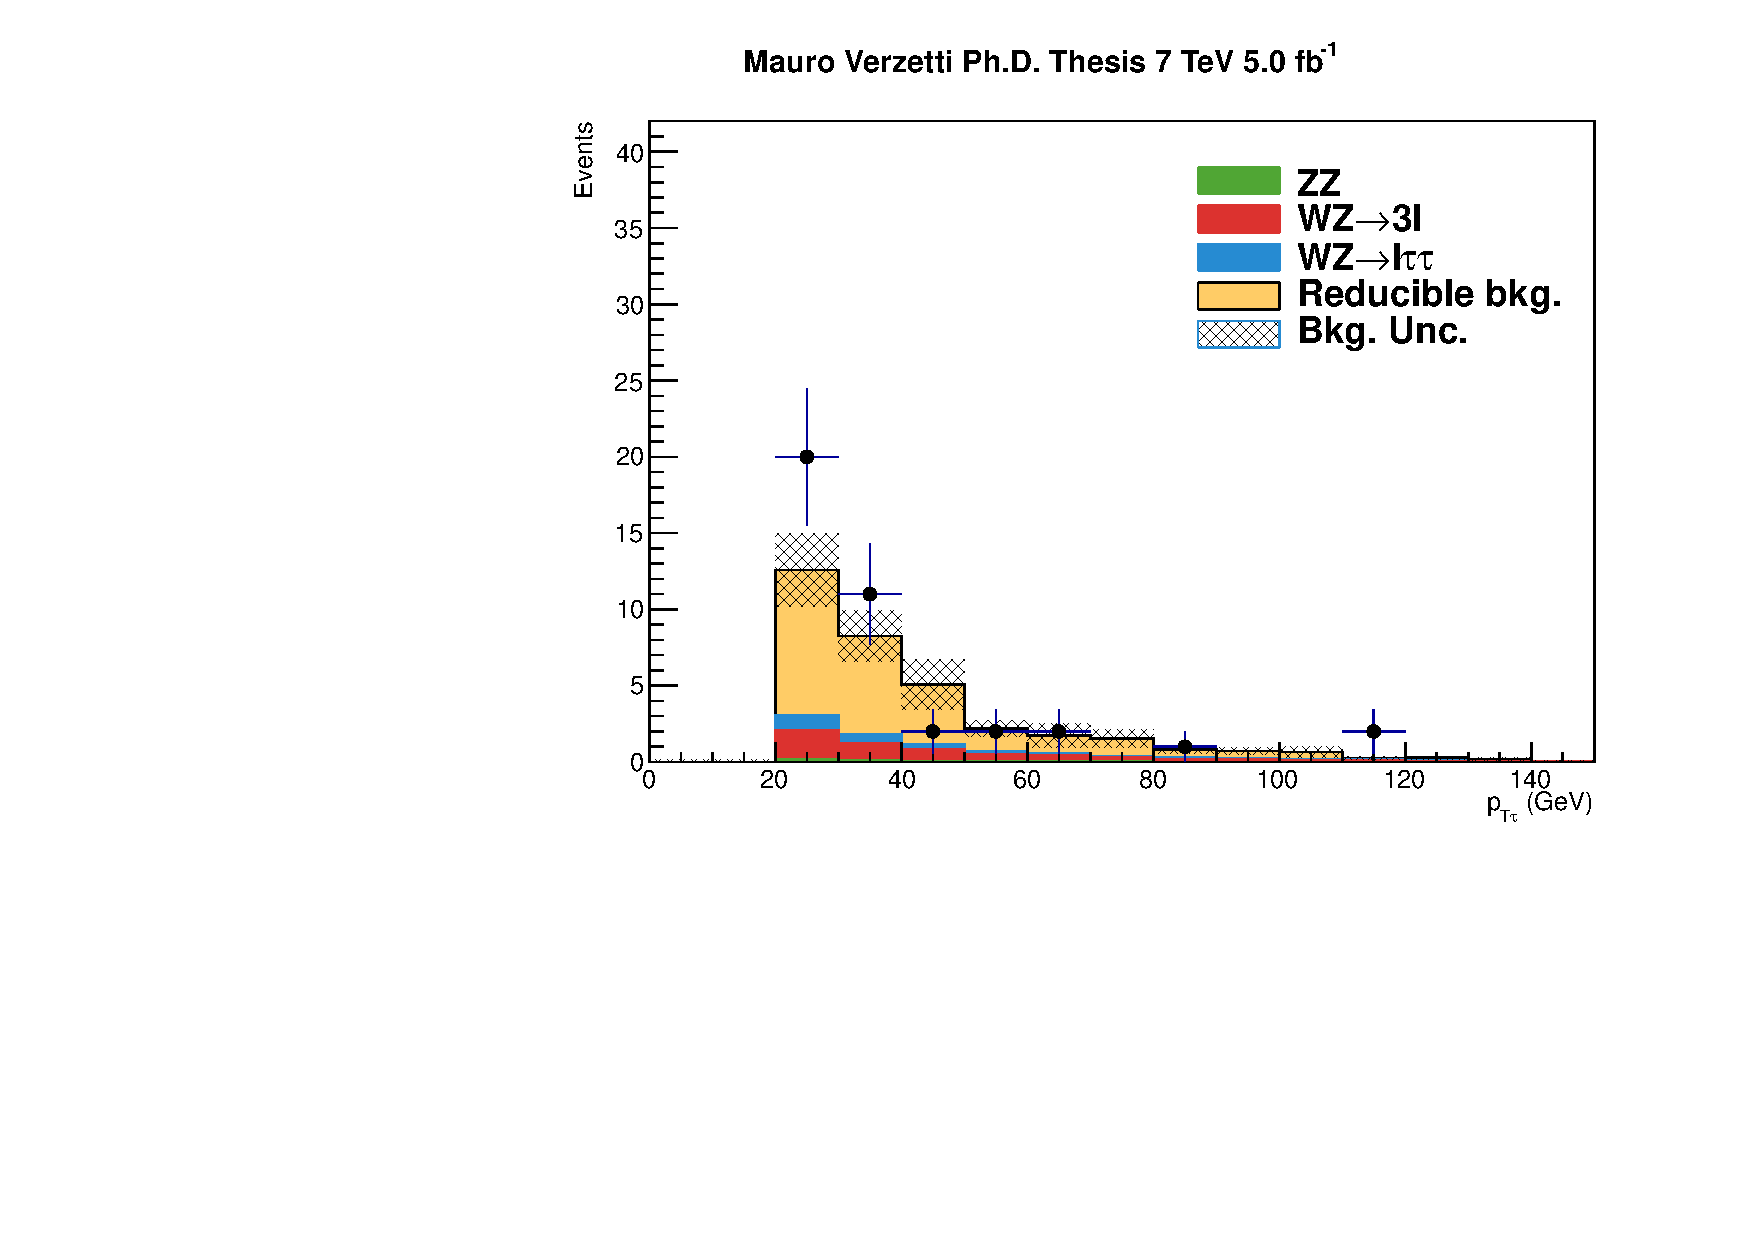
\includegraphics[width=0.49\textwidth]{4_Analisys/pics/7TeV/plots/mmt/f3/Full/final-f3-tPt-Full.pdf}
  \caption{Comparison of measured and predicted backgrounds in the $\mu\mu\tau_h$ ``fake tau'' control region for 7 TeV data.
  From top left to bottom: mass of the sub-leading muon and the tau system, scalar sum of the leptons \pT ($L_T$), \pT of the leading and sub-leading muon, and \pT of the hadronic tau.
  The reducible background contribution is estimated by the kNN method, as in the signal region.
  The shaded band represents the uncertainty on the sum of the background contributions.
  }
  \label{fig:LLT_mmt_f3_control_7TeV}
\end{center}
\end{figure}

\begin{figure}
\begin{center}
  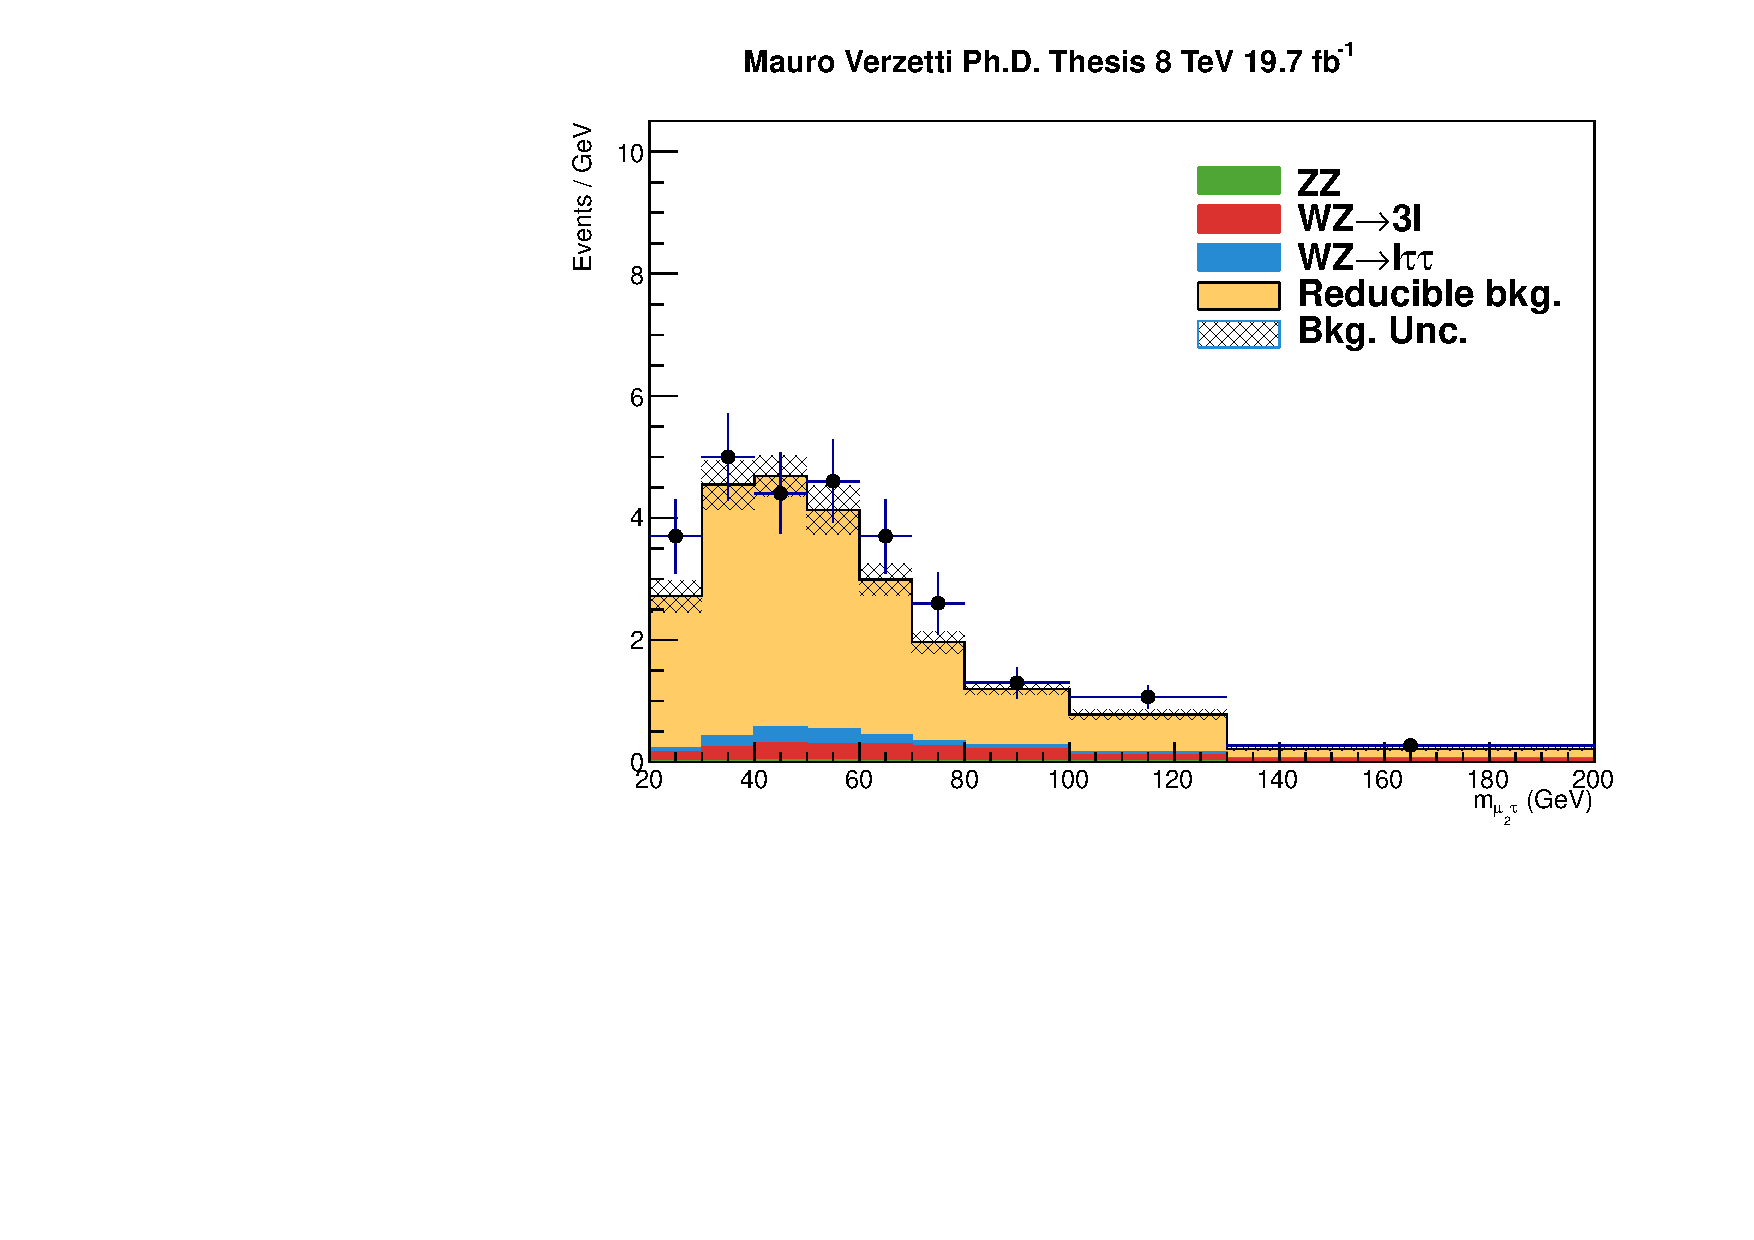
\includegraphics[width=0.49\textwidth]{4_Analisys/pics/8TeV/plots/mmt/f3/Full/final-f3-subMass-Full.pdf}
  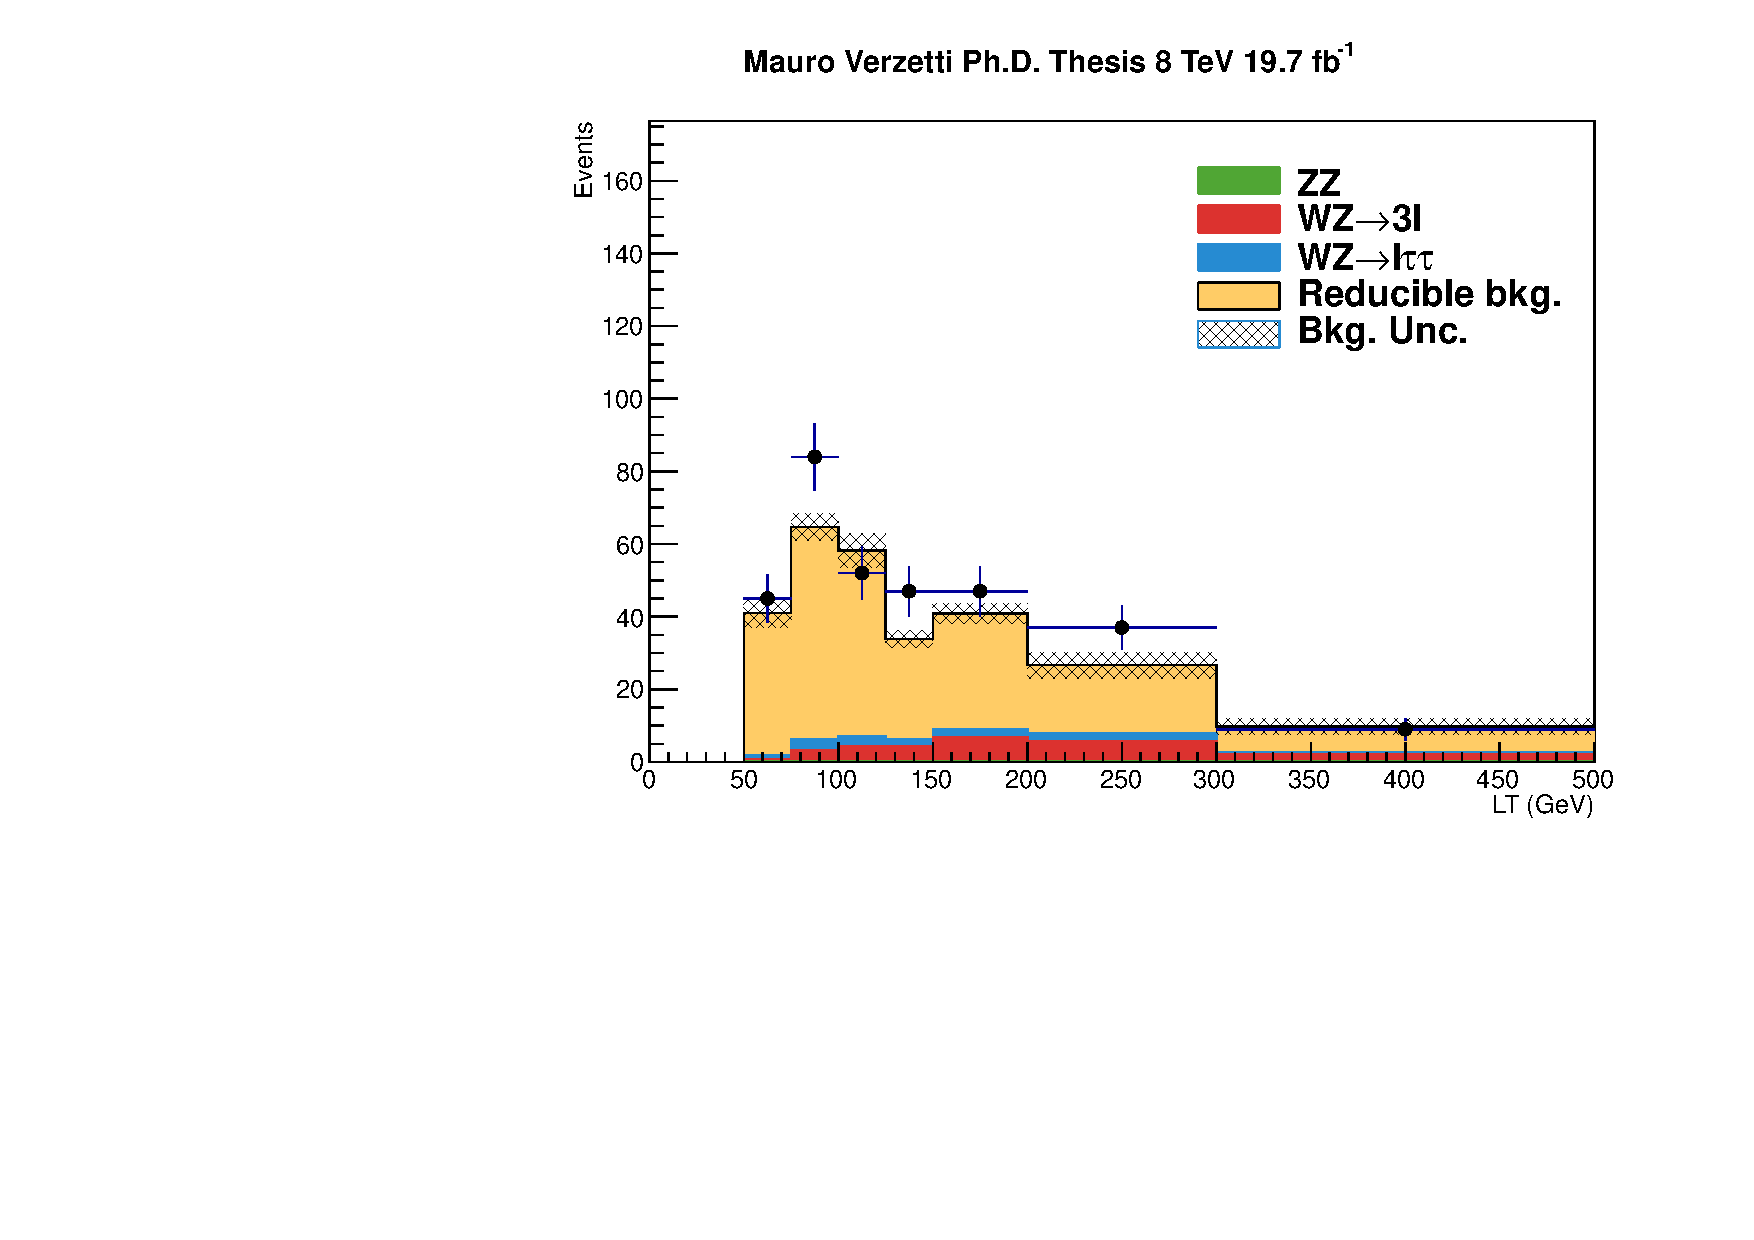
\includegraphics[width=0.49\textwidth]{4_Analisys/pics/8TeV/plots/mmt/f3/final-LT.pdf}\\
  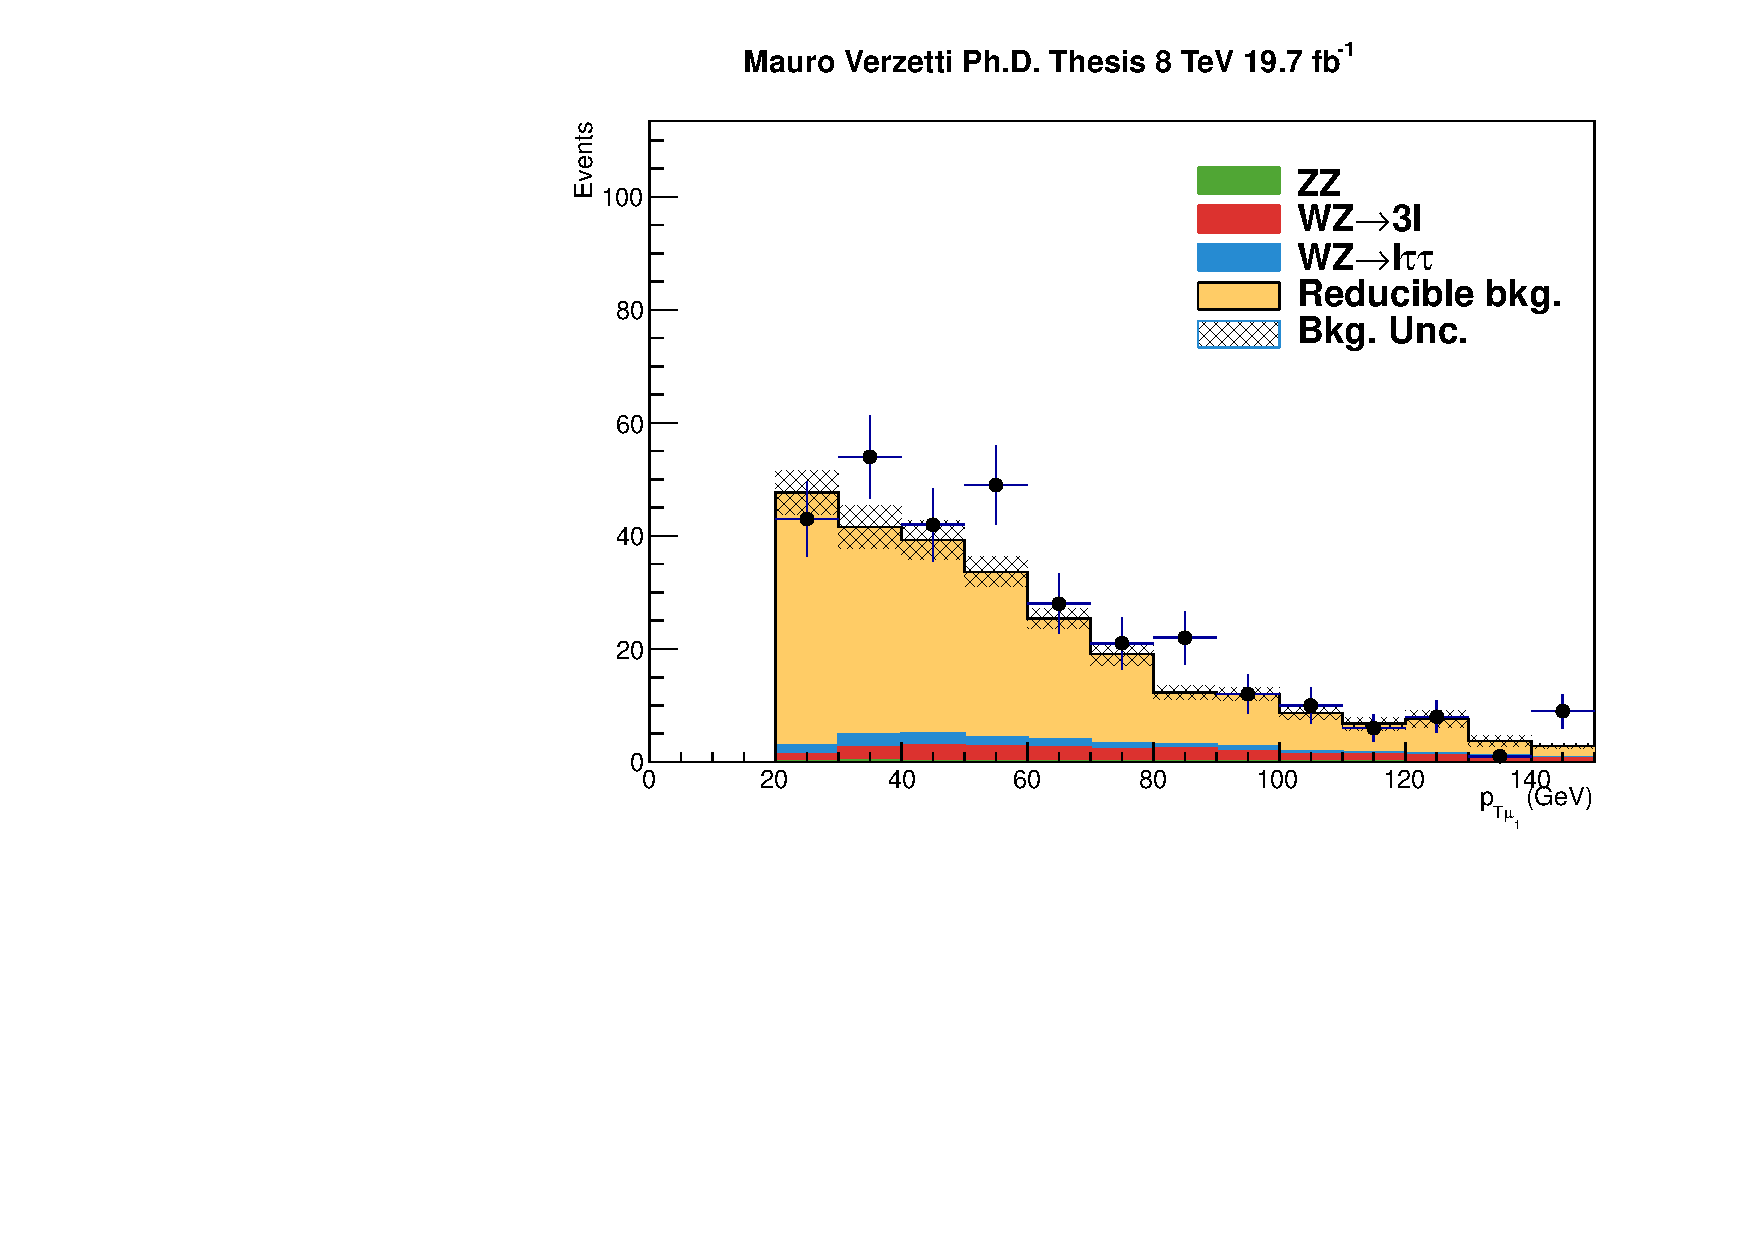
\includegraphics[width=0.49\textwidth]{4_Analisys/pics/8TeV/plots/mmt/f3/Full/final-f3-m1Pt-Full.pdf}
  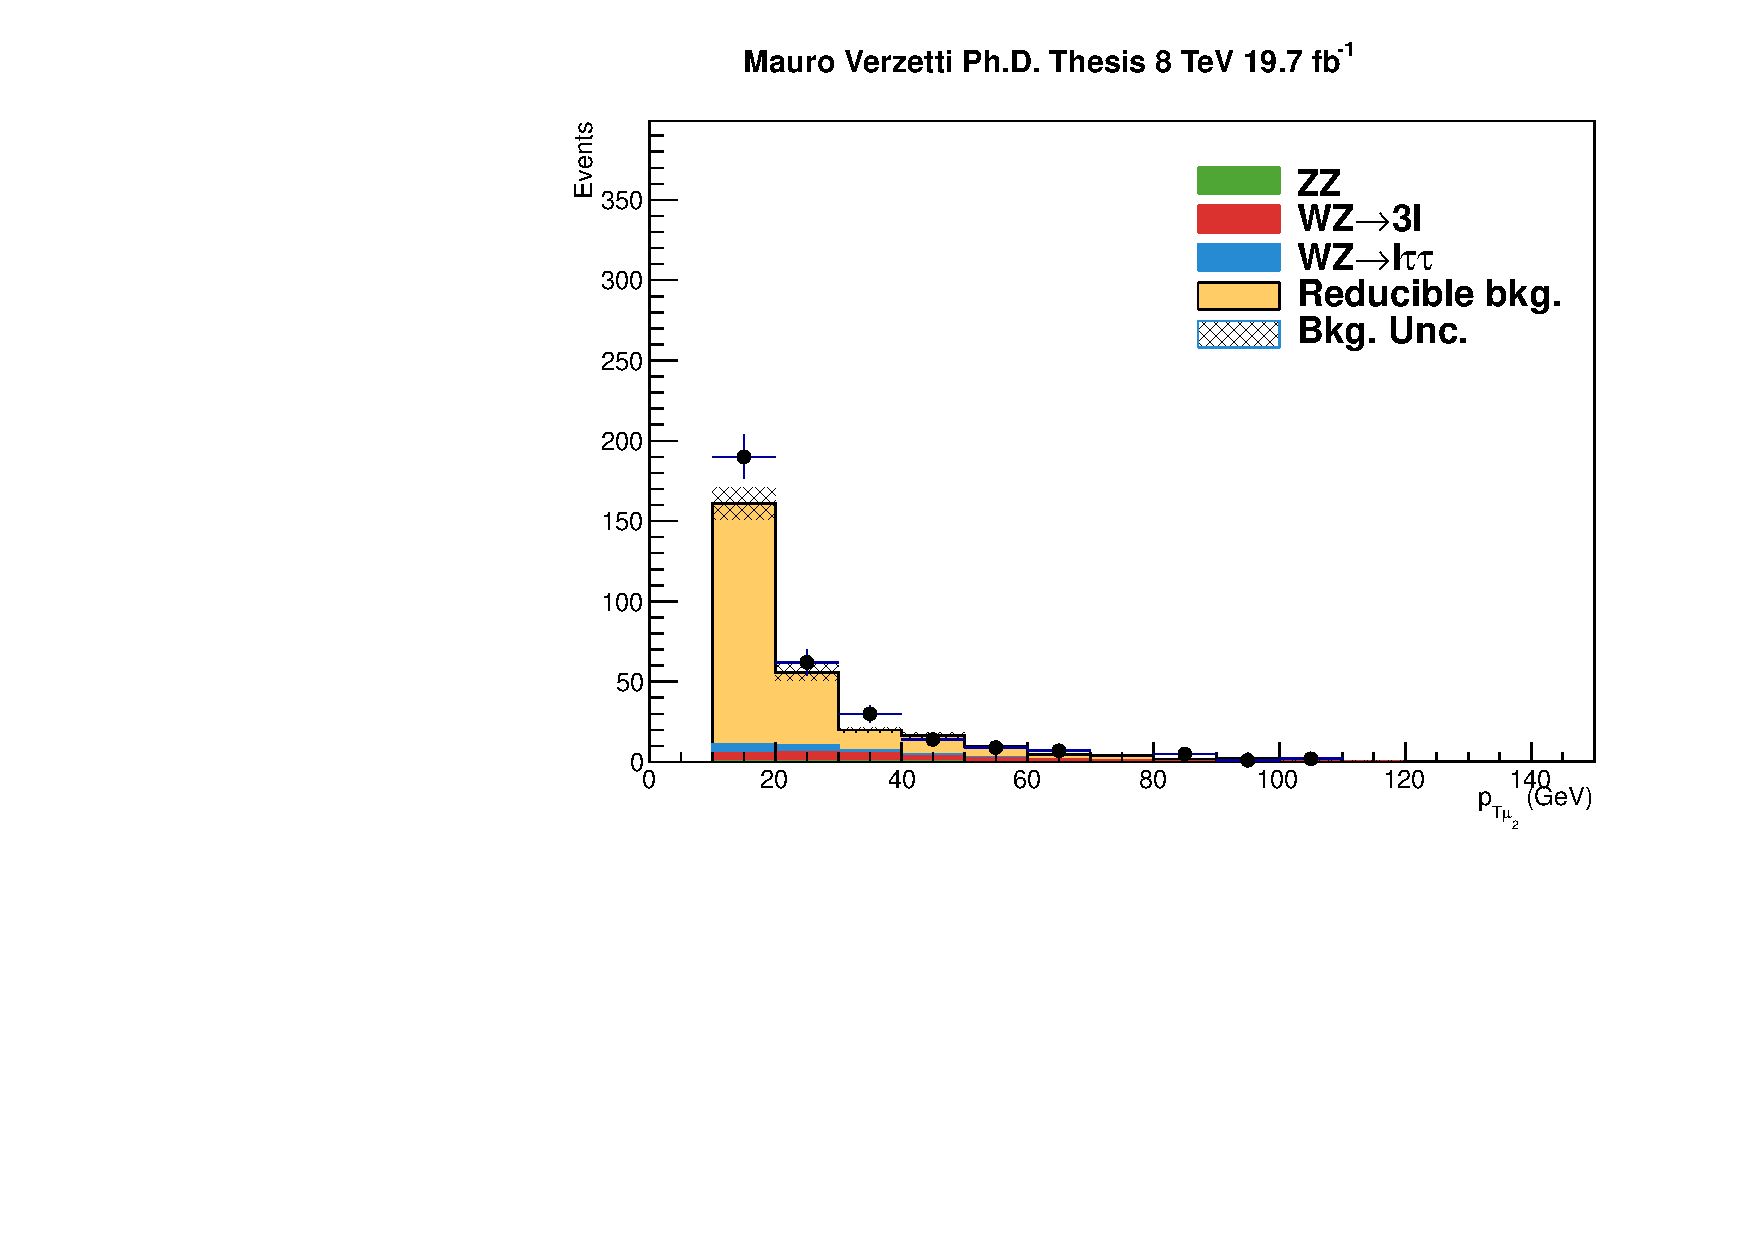
\includegraphics[width=0.49\textwidth]{4_Analisys/pics/8TeV/plots/mmt/f3/Full/final-f3-m2Pt-Full.pdf}\\
  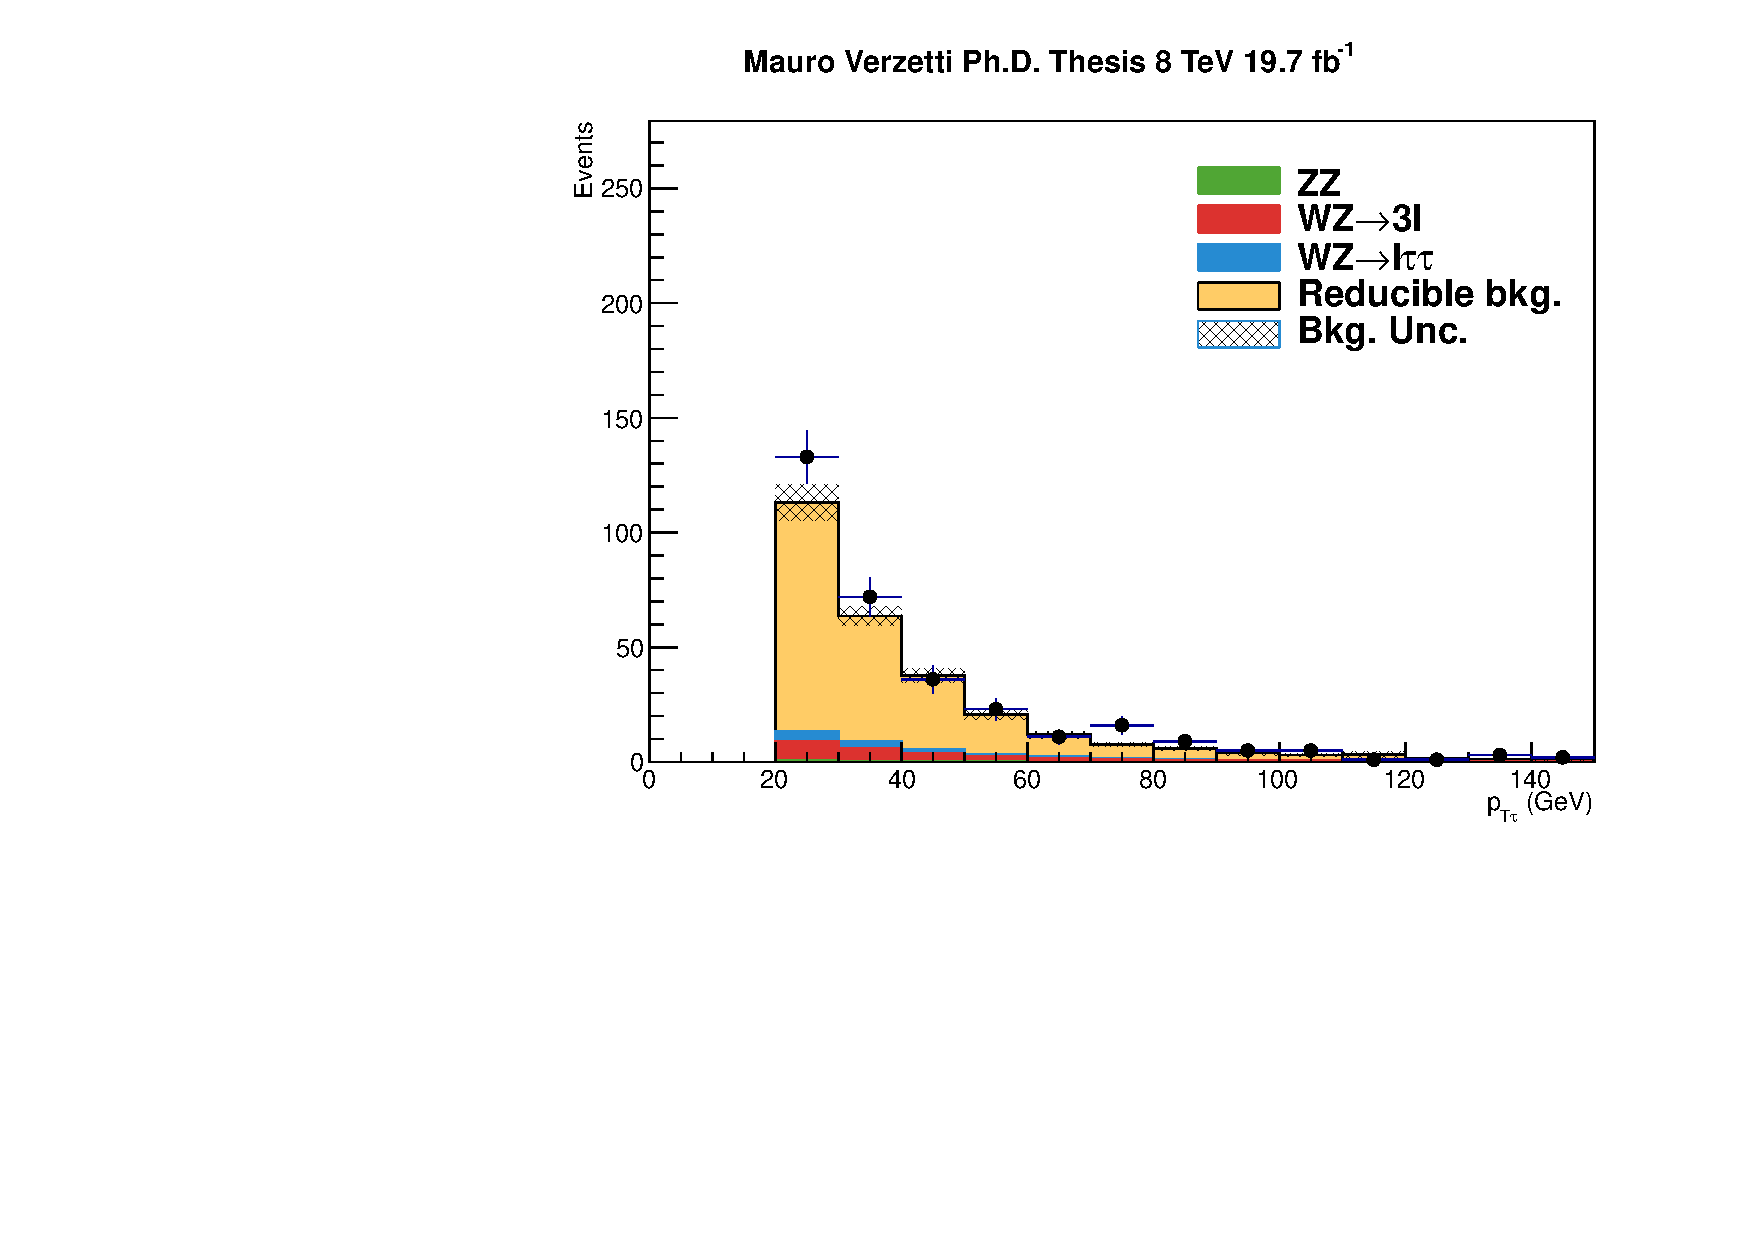
\includegraphics[width=0.49\textwidth]{4_Analisys/pics/8TeV/plots/mmt/f3/Full/final-f3-tPt-Full.pdf}
  \caption{Comparison of measured and predicted backgrounds in the $\mu\mu\tau_h$ ``fake tau'' control region for 8 TeV data.
  From top left to bottom: mass of the sub-leading muon and the tau system, scalar sum of the leptons \pT ($L_T$), \pT of the leading and sub-leading muon, and \pT of the hadronic tau.
  The reducible background contribution is estimated by the kNN method, as in the signal region.
  The shaded band represents the uncertainty on the sum of the background contributions.
  }
  \label{fig:LLT_mmt_f3_control_8TeV}
\end{center}
\end{figure}

\begin{figure}
\begin{center}
  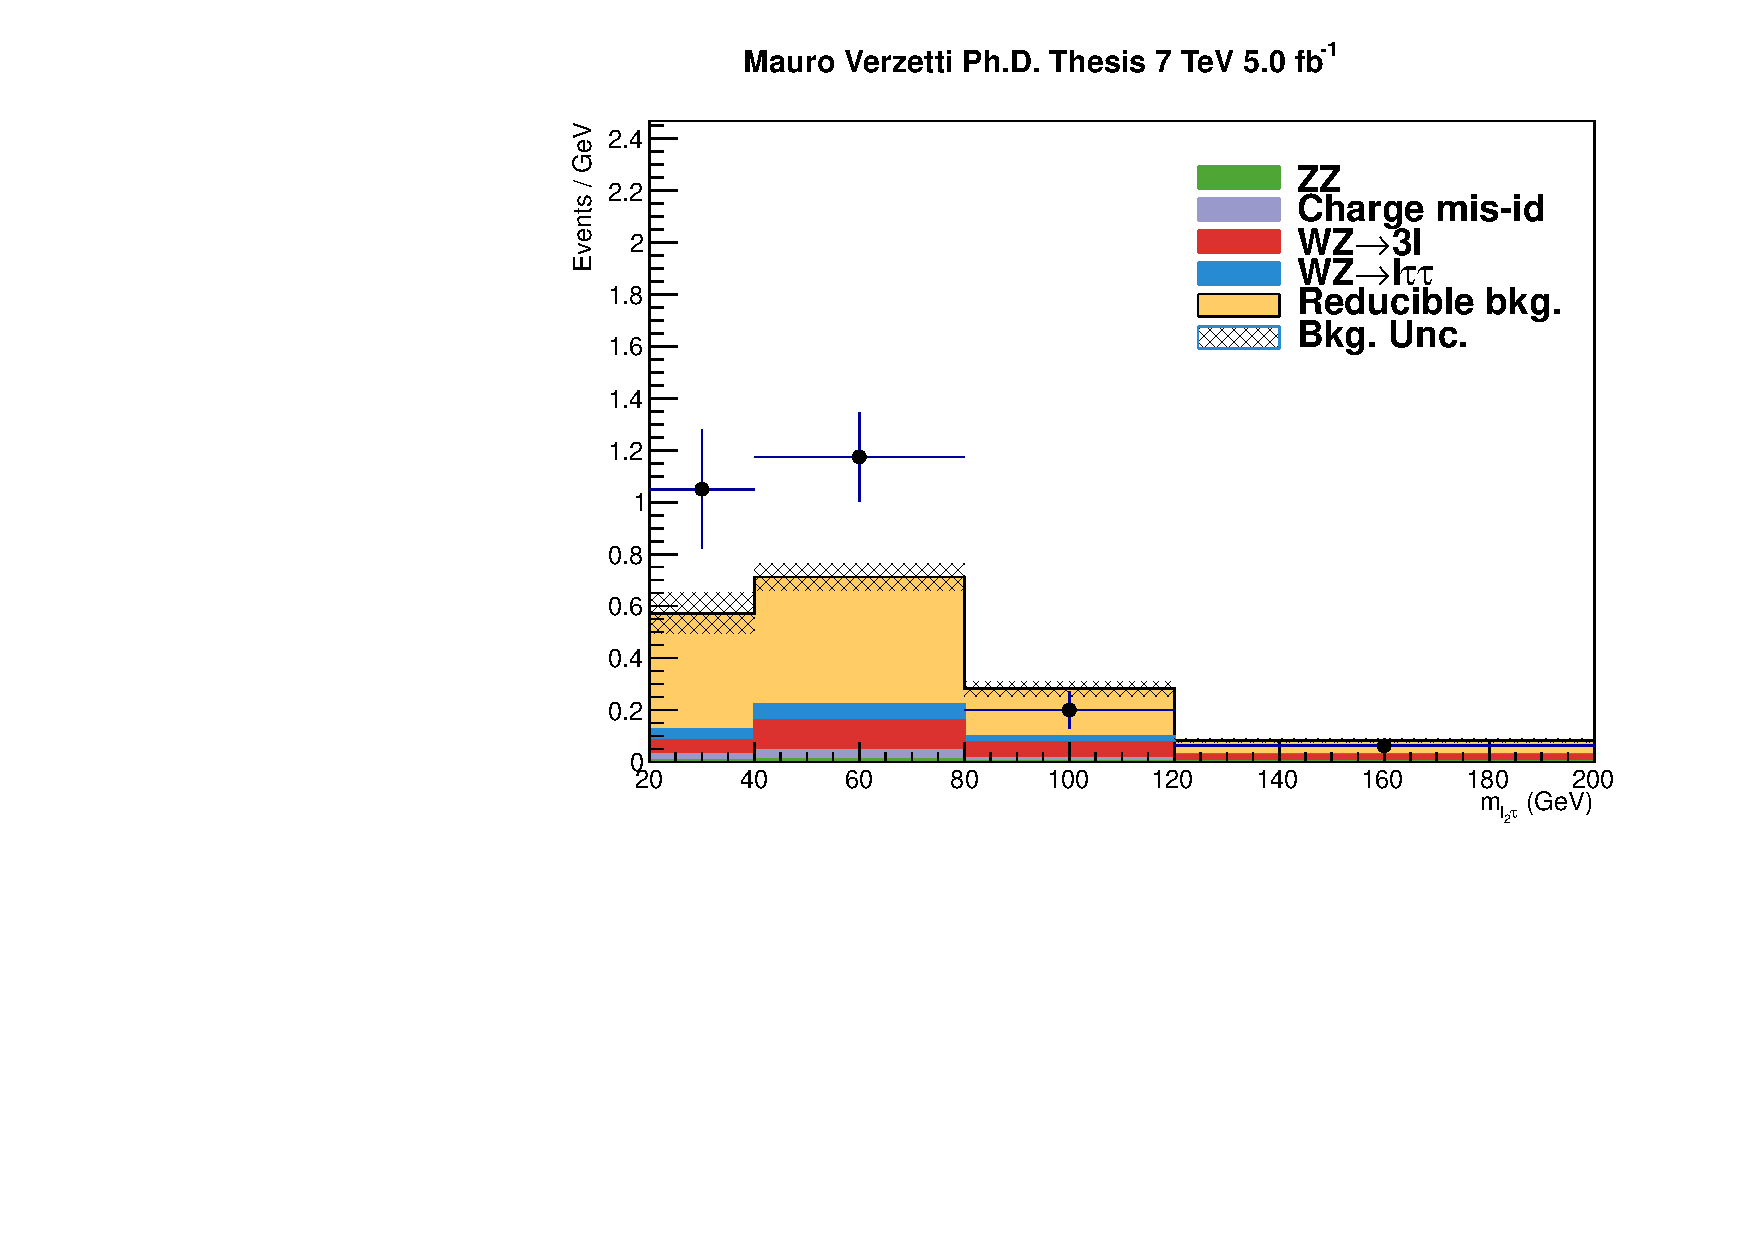
\includegraphics[width=0.49\textwidth]{4_Analisys/pics/7TeV/plots/emt/f3/Full/final-f3-subMass-Full.pdf}
  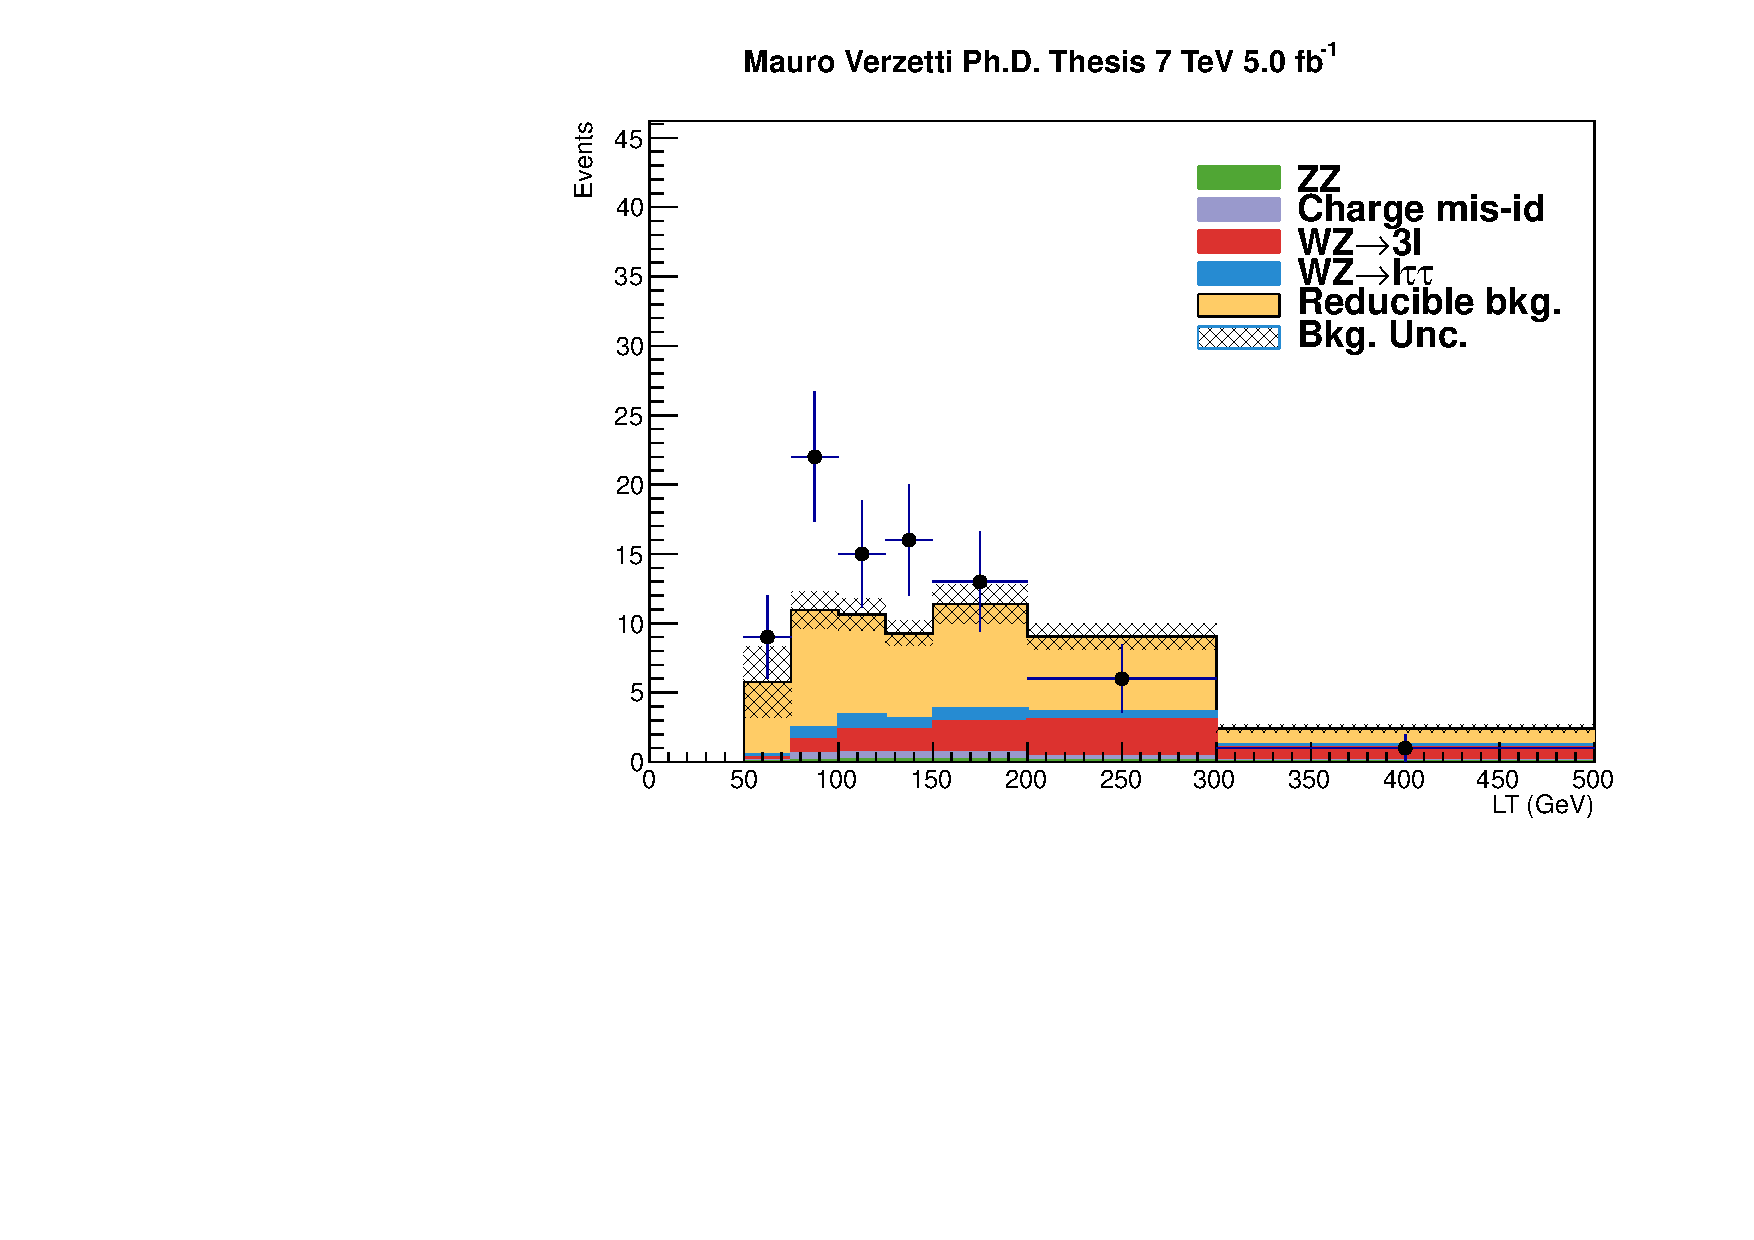
\includegraphics[width=0.49\textwidth]{4_Analisys/pics/7TeV/plots/emt/f3/final-f3-LT.pdf}\\
  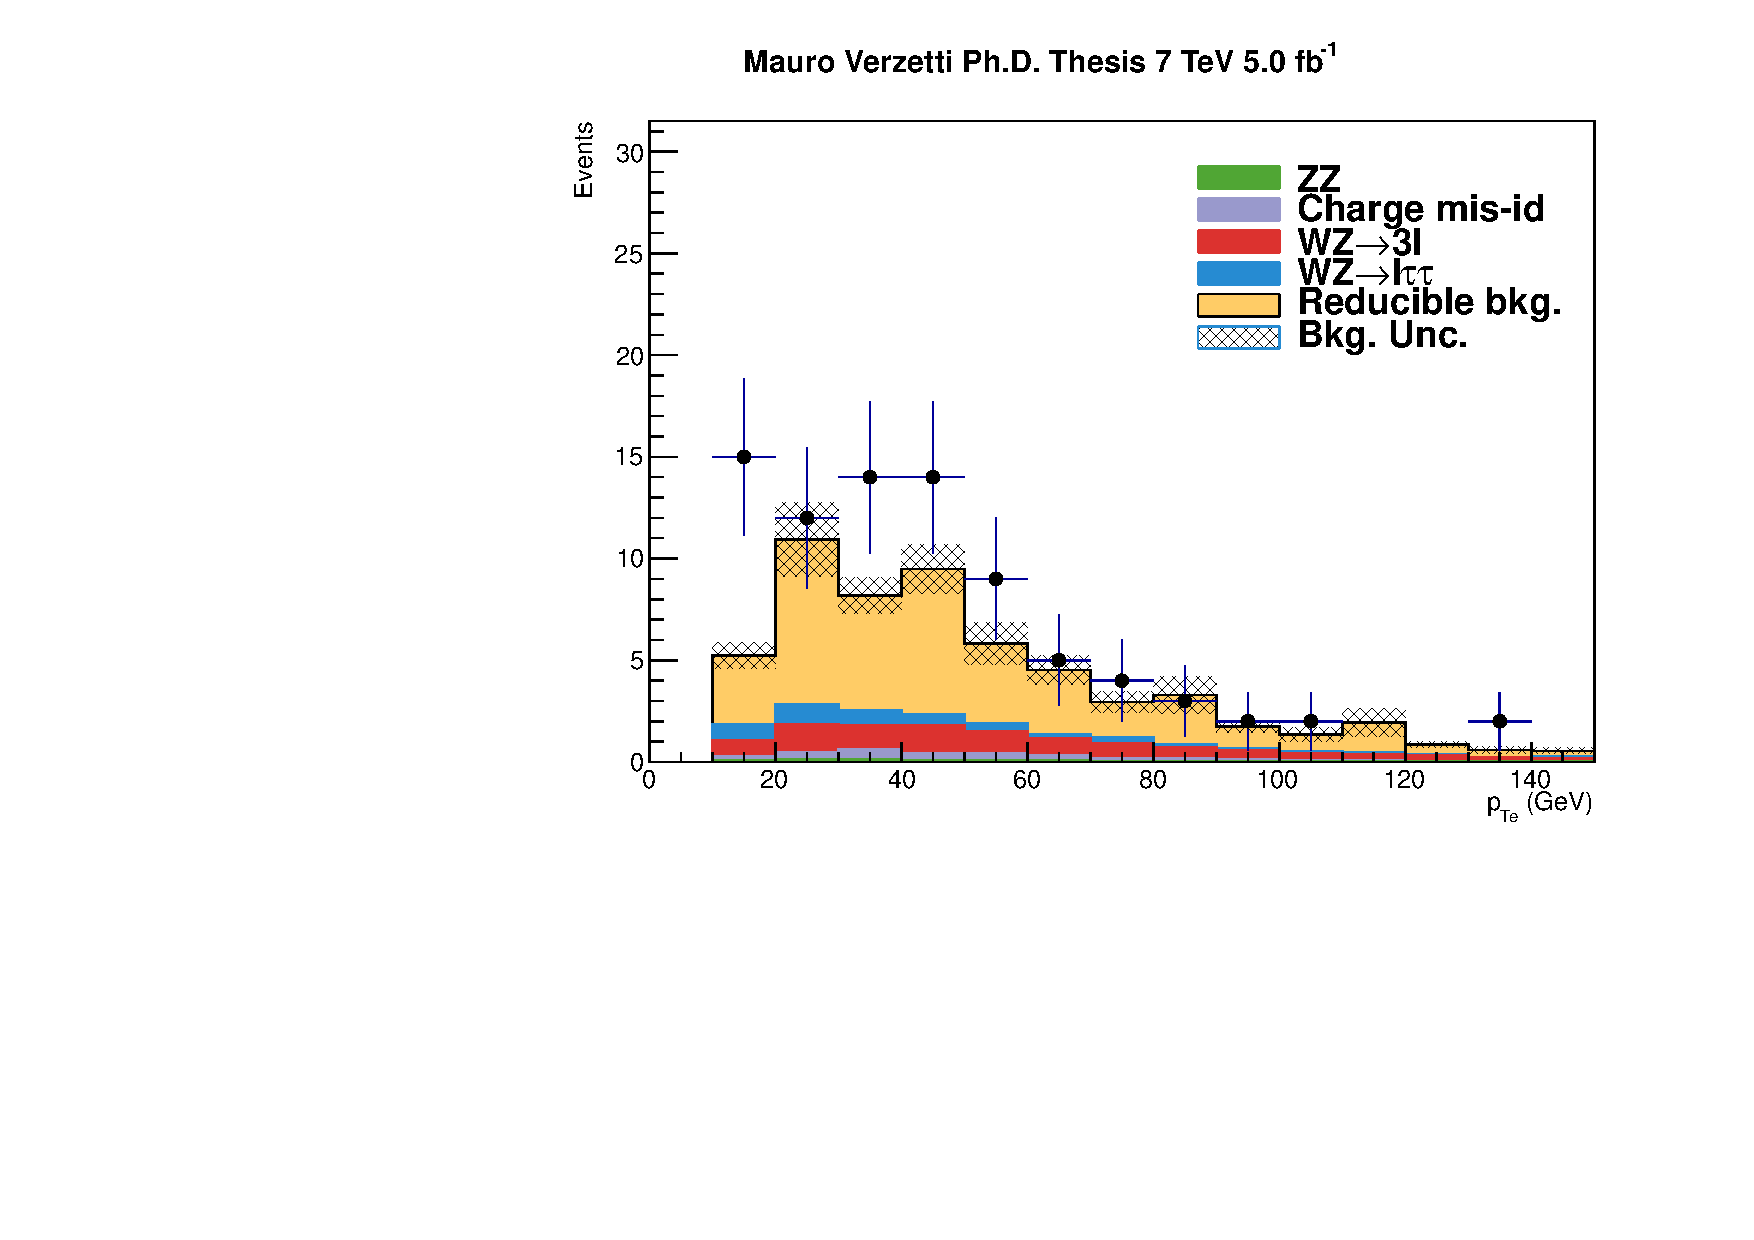
\includegraphics[width=0.49\textwidth]{4_Analisys/pics/7TeV/plots/emt/f3/Full/final-f3-ePt-Full.pdf}
  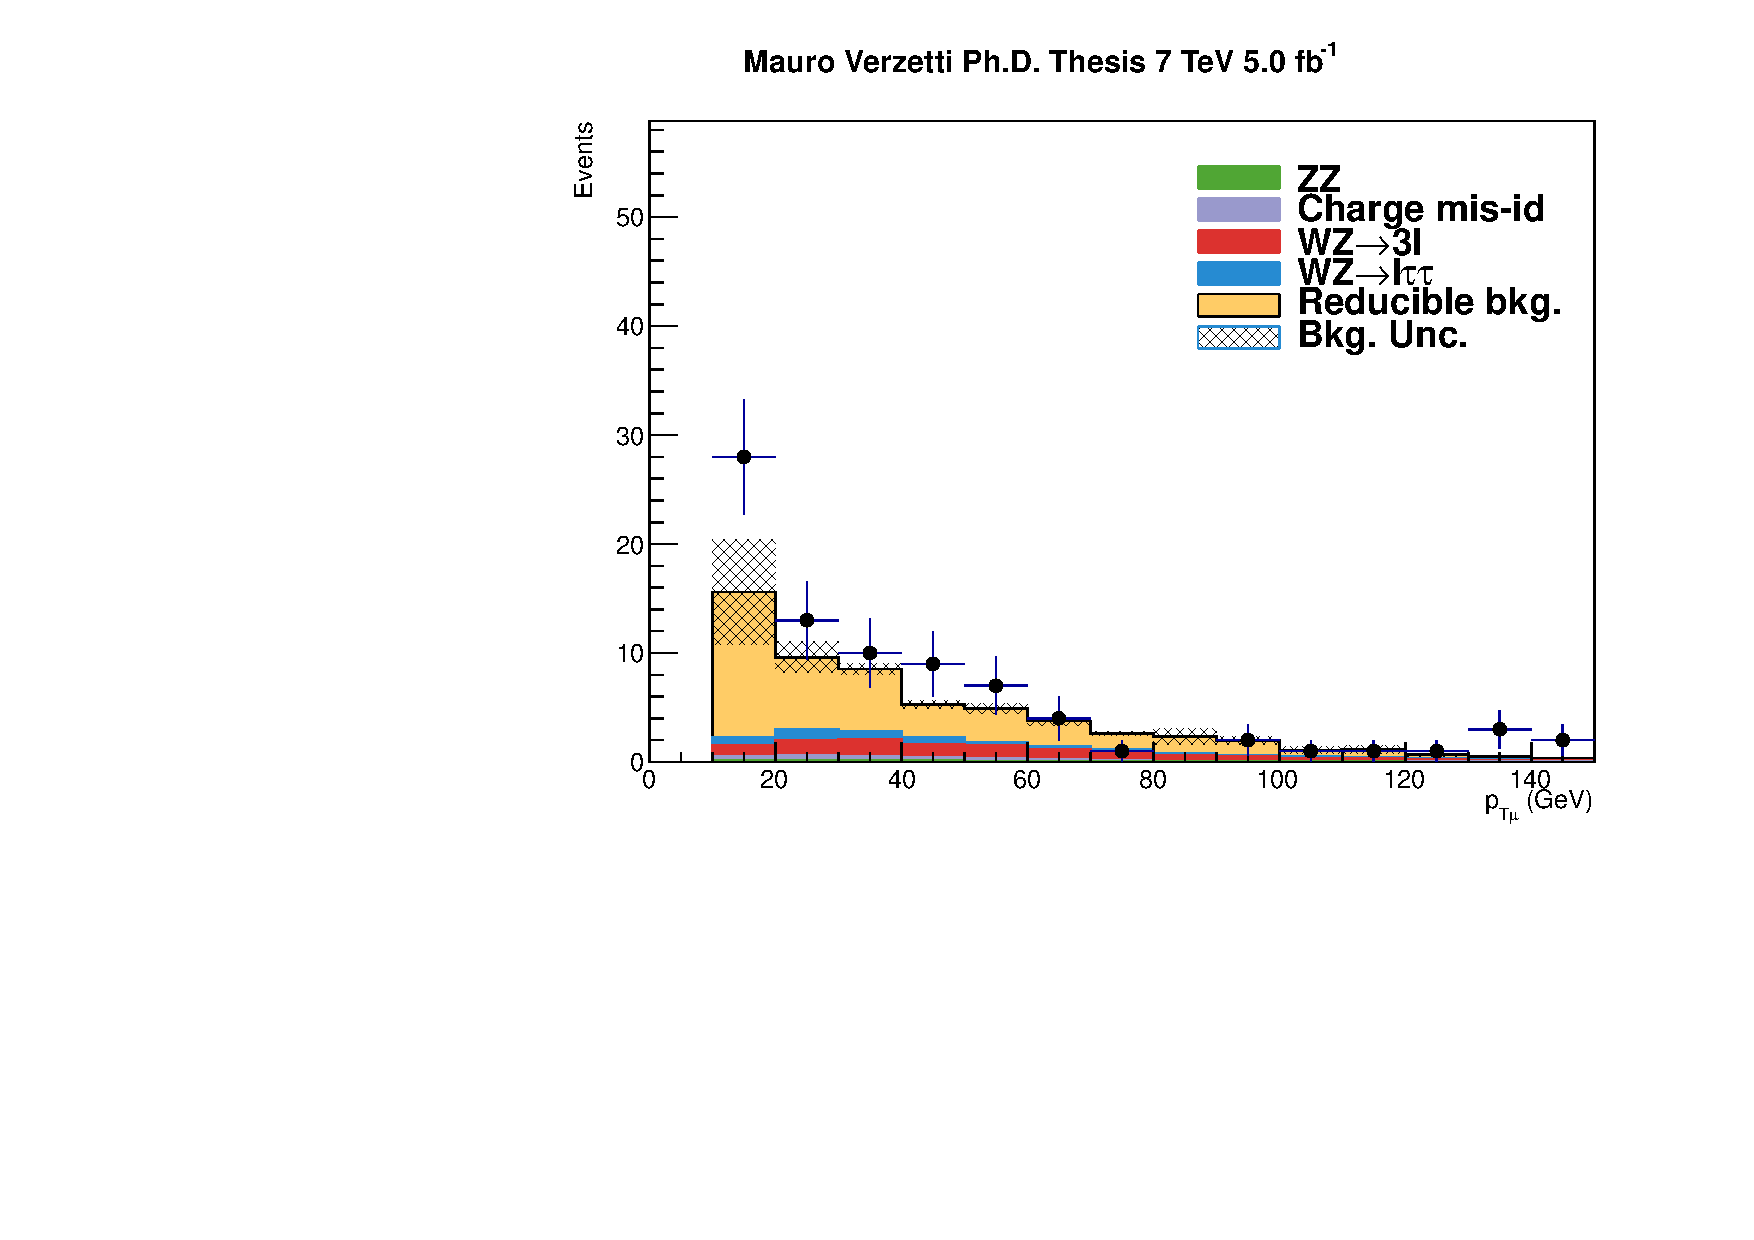
\includegraphics[width=0.49\textwidth]{4_Analisys/pics/7TeV/plots/emt/f3/Full/final-f3-mPt-Full.pdf}\\
  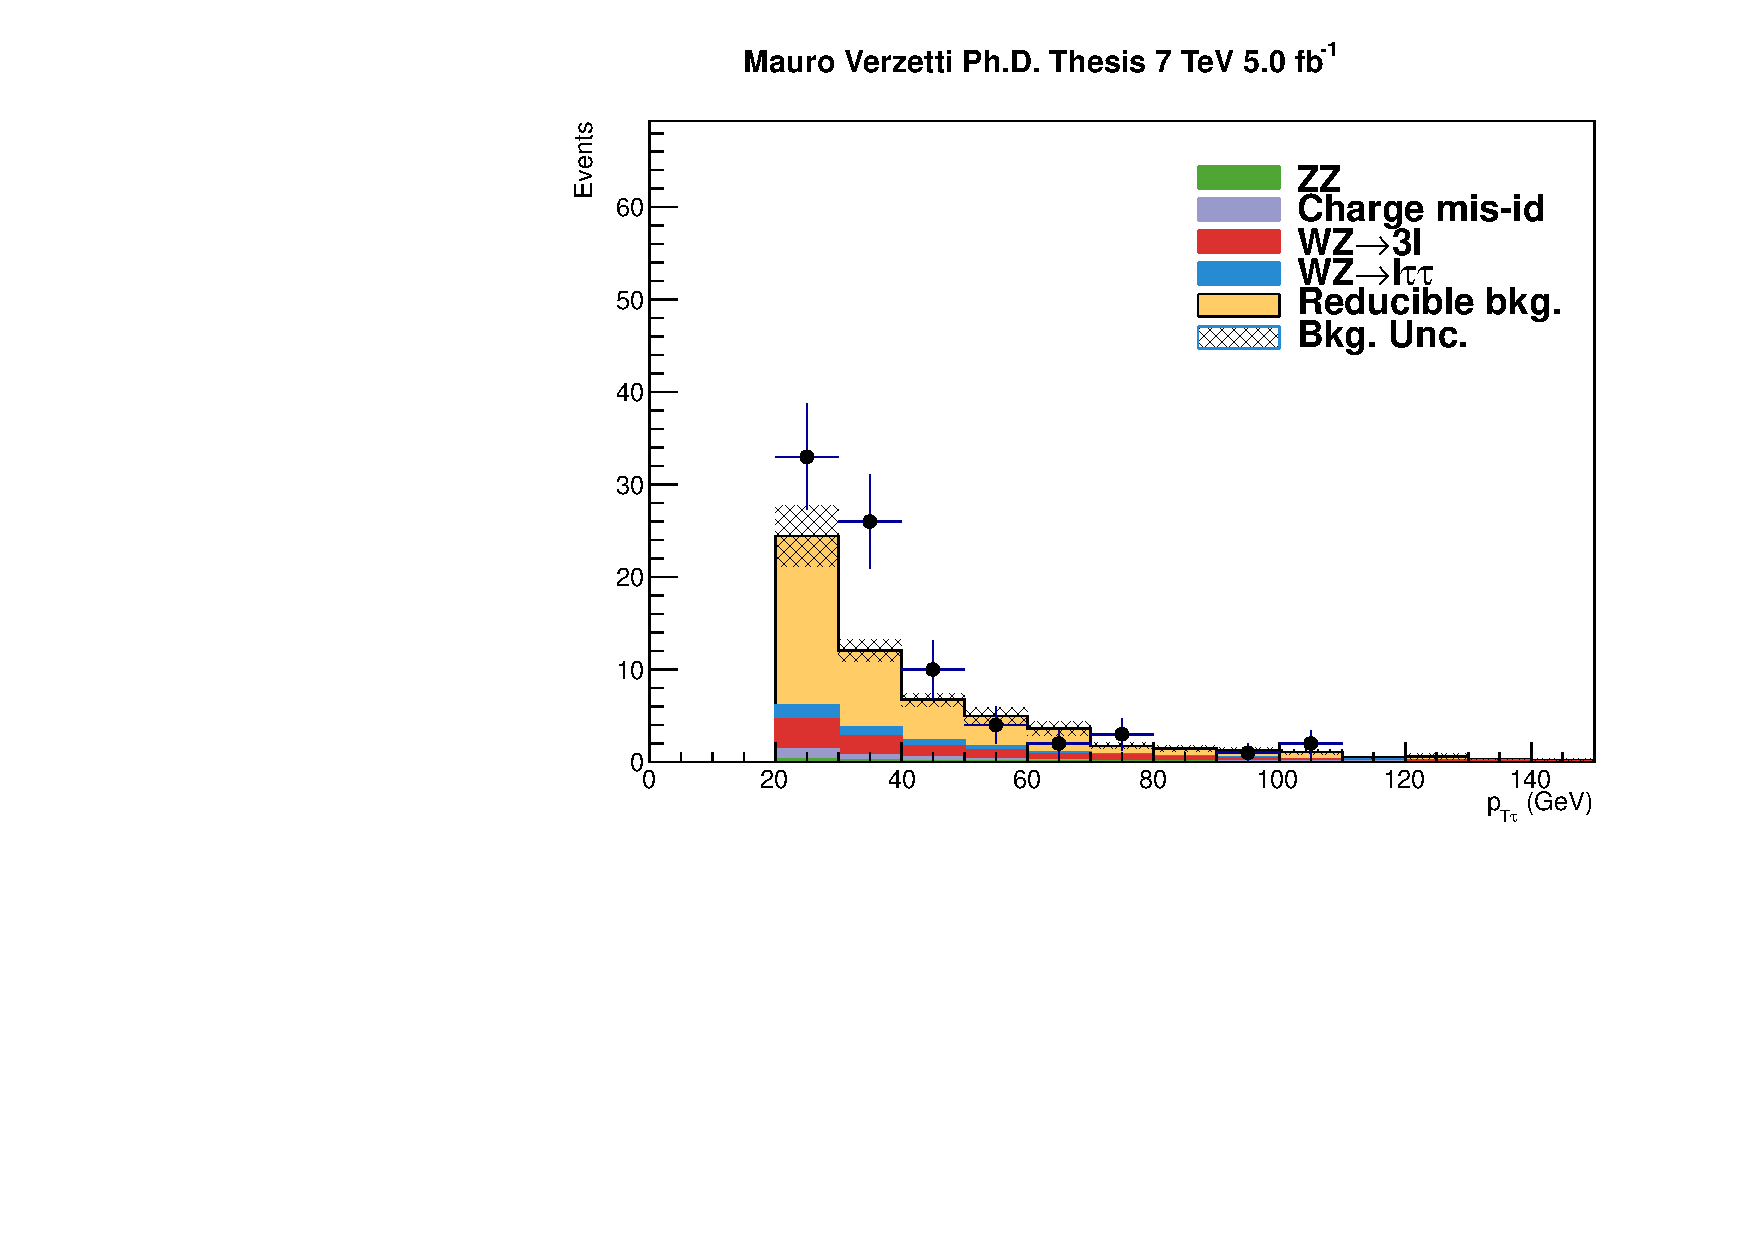
\includegraphics[width=0.49\textwidth]{4_Analisys/pics/7TeV/plots/emt/f3/Full/final-f3-tPt-Full.pdf}
  \caption{Comparison of measured and predicted backgrounds in the $e\mu\tau_h$ ``fake tau'' control region for 7 TeV data.
  From top left to bottom: mass of the sub-leading lepton and the tau system, scalar sum of the leptons \pT ($L_T$), \pT of the electron, muon, and hadronic tau.
  The reducible background contribution is estimated by the kNN method, as in the signal region.
  The shaded band represents the uncertainty on the sum of the background contributions.
  }
  \label{fig:LLT_emt_f3_control_7TeV}
\end{center}
\end{figure}

\begin{figure}
\begin{center}
  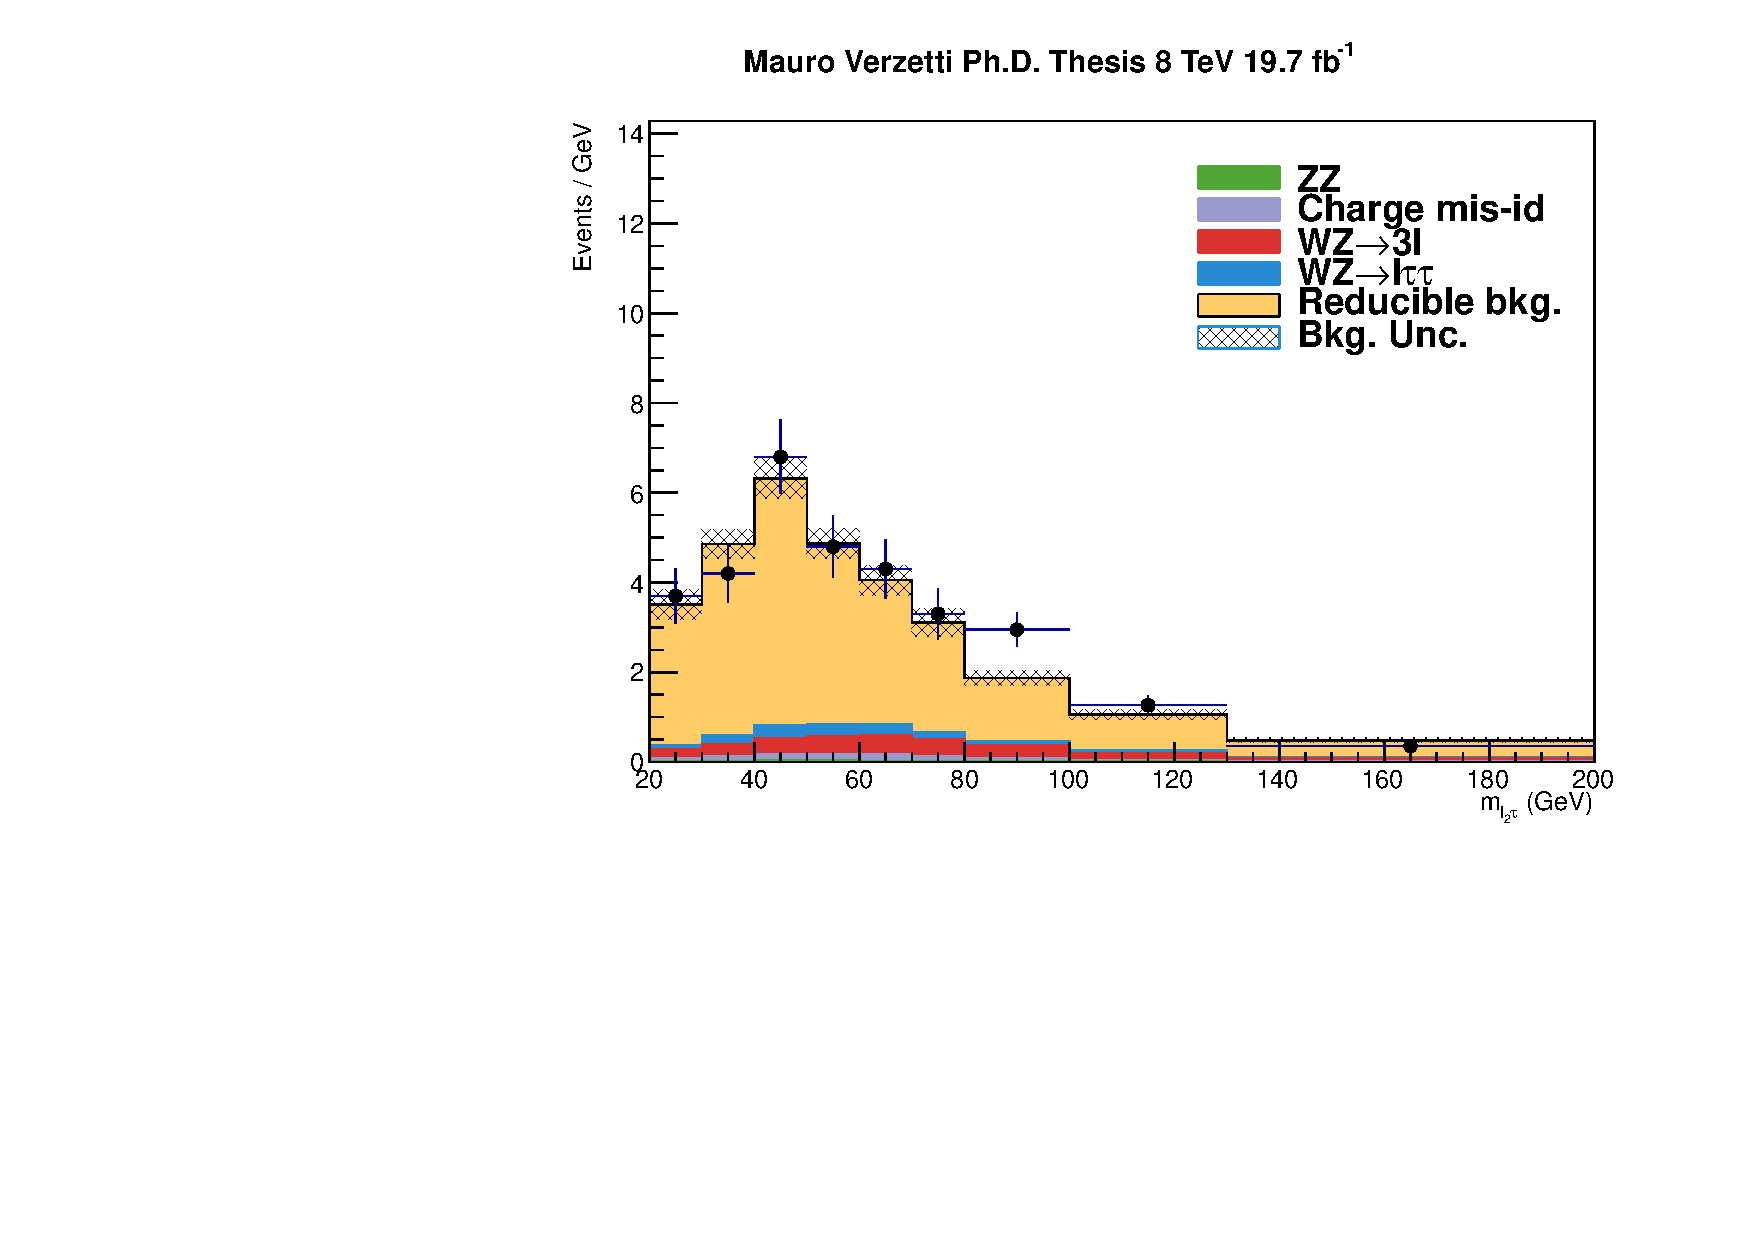
\includegraphics[width=0.49\textwidth]{4_Analisys/pics/8TeV/plots/emt/f3/Full/final-f3-subMass-Full.pdf}
  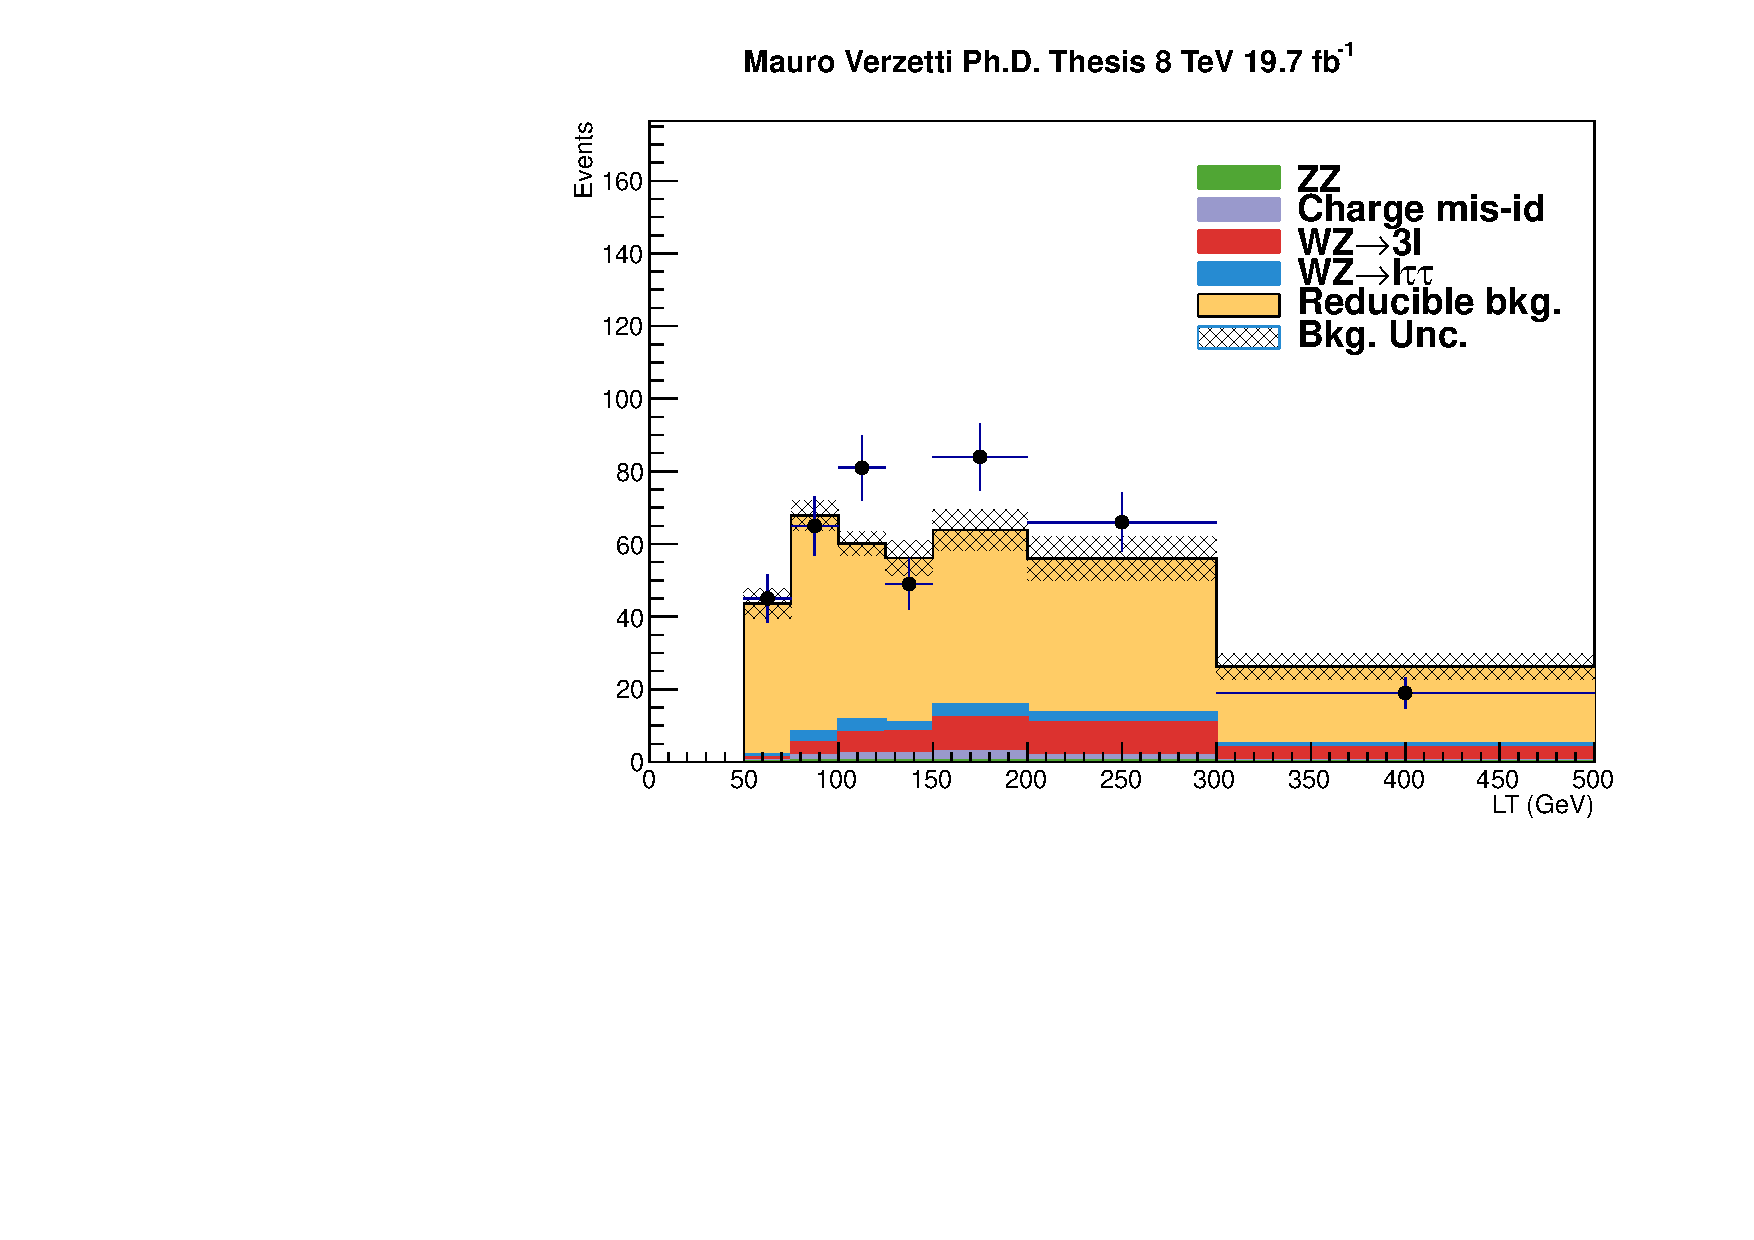
\includegraphics[width=0.49\textwidth]{4_Analisys/pics/8TeV/plots/emt/f3/final-f3-LT.pdf}\\
  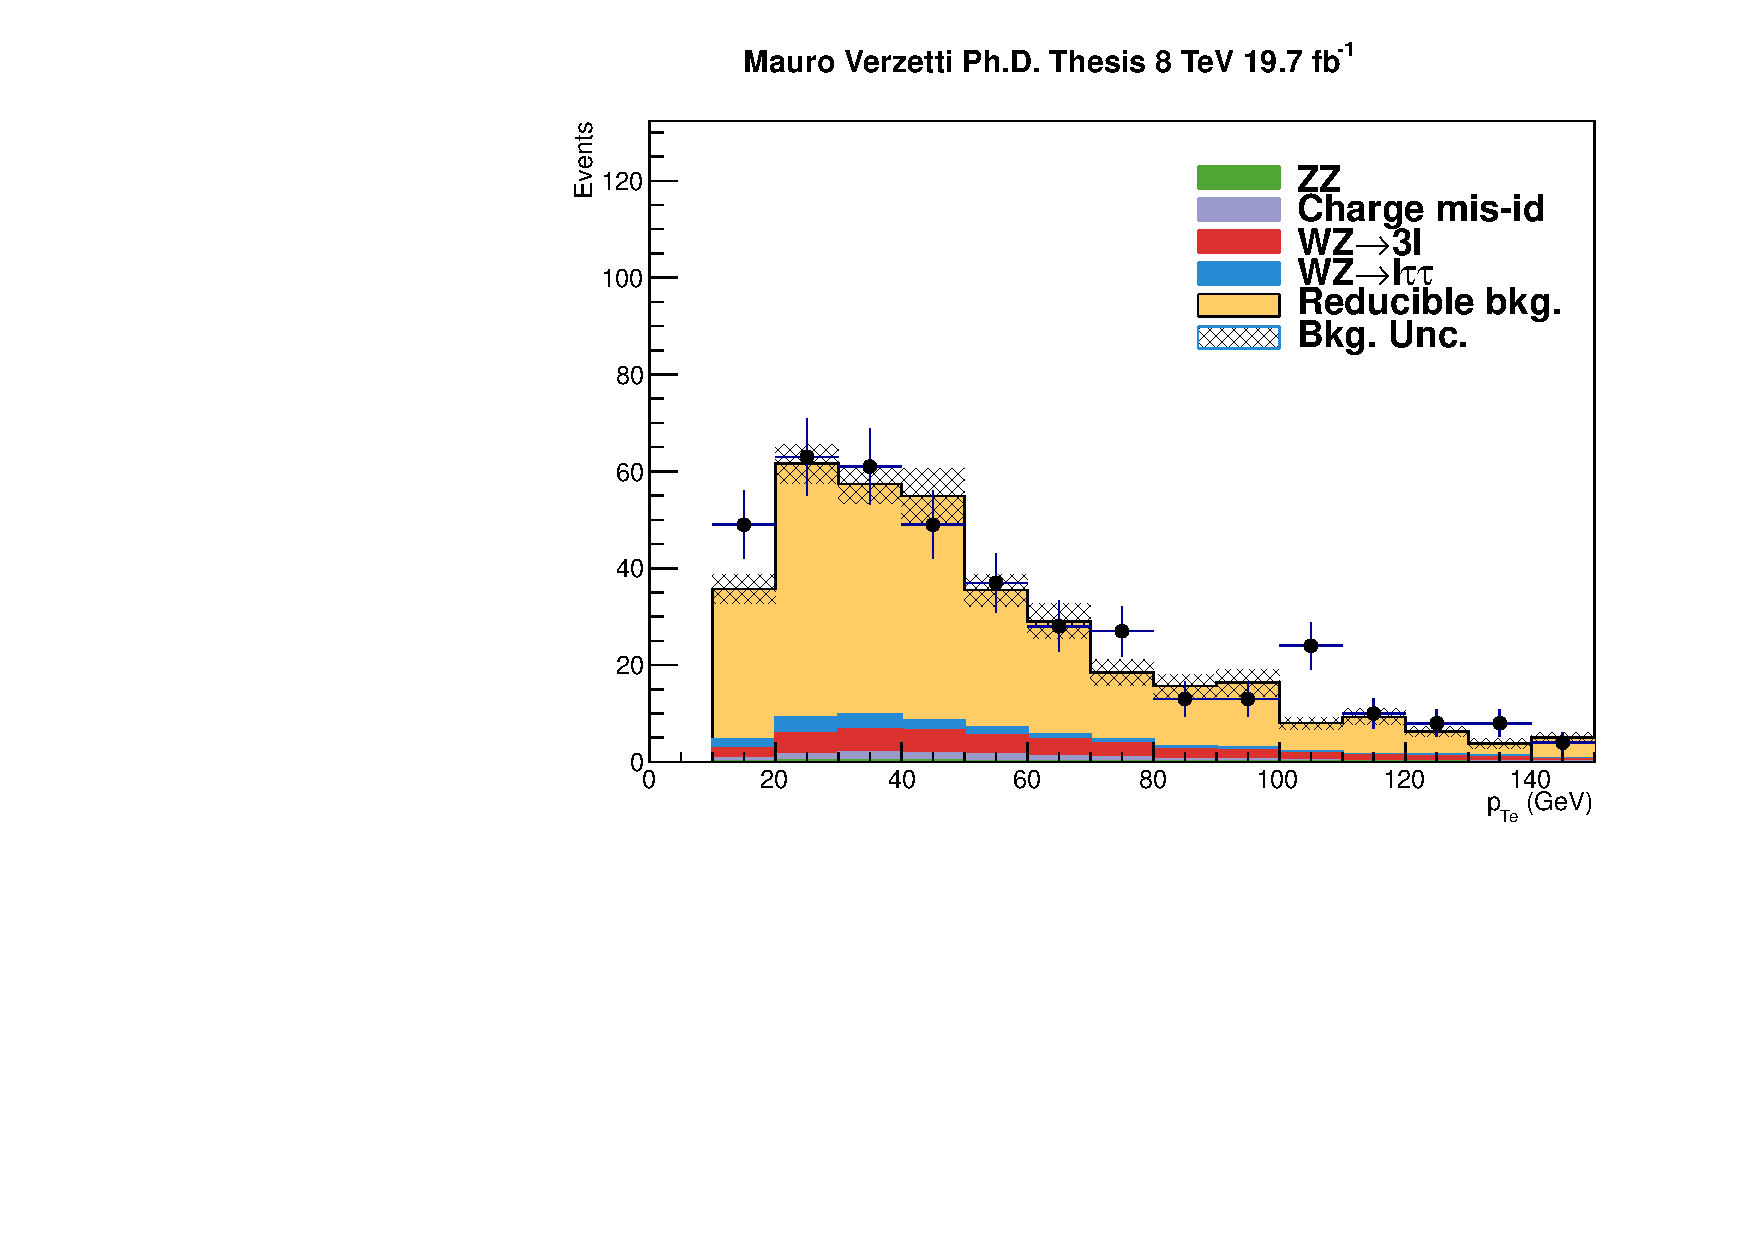
\includegraphics[width=0.49\textwidth]{4_Analisys/pics/8TeV/plots/emt/f3/Full/final-f3-ePt-Full.pdf}
  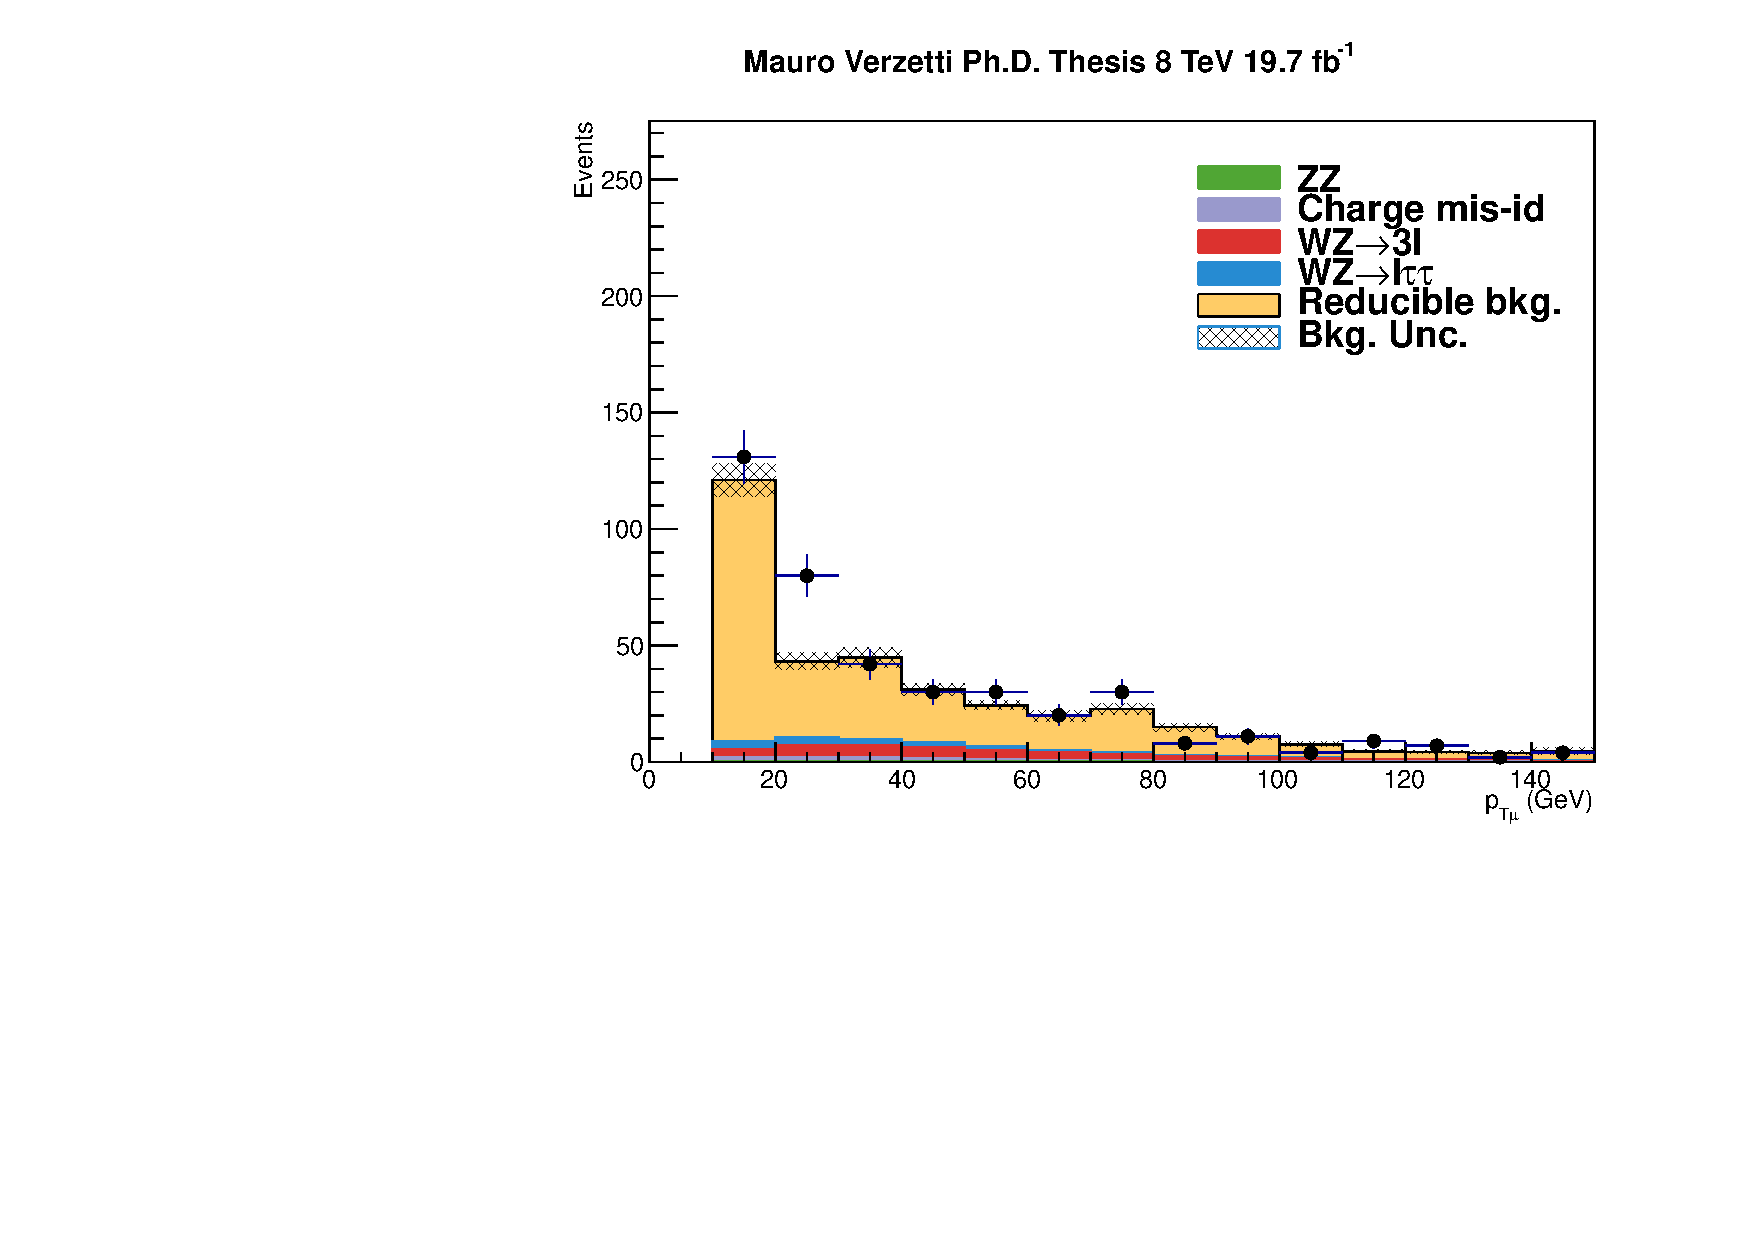
\includegraphics[width=0.49\textwidth]{4_Analisys/pics/8TeV/plots/emt/f3/Full/final-f3-mPt-Full.pdf}\\
  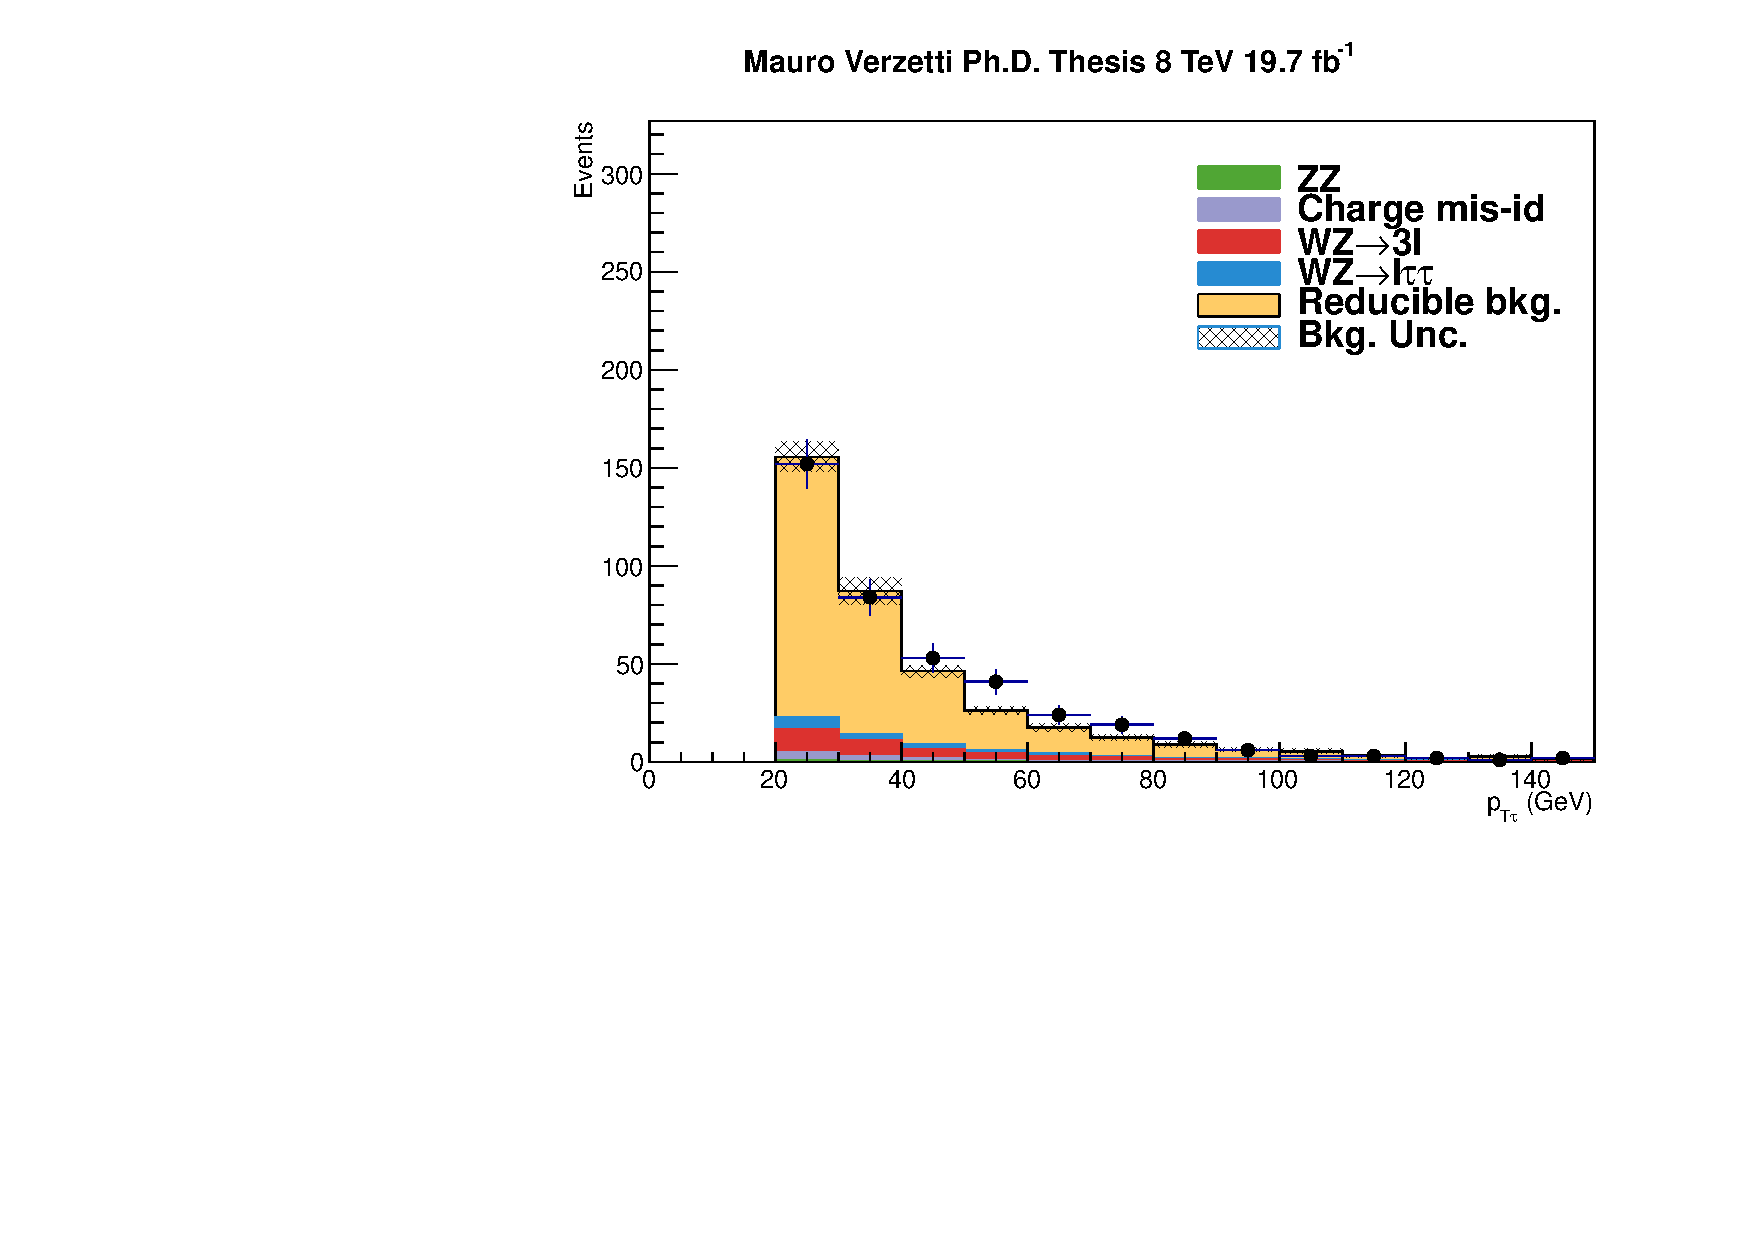
\includegraphics[width=0.49\textwidth]{4_Analisys/pics/8TeV/plots/emt/f3/Full/final-f3-tPt-Full.pdf}
  \caption{Comparison of measured and predicted backgrounds in the $e\mu\tau_h$ ``fake tau'' control region for 8 TeV data.
  From top left to bottom: mass of the sub-leading lepton and the tau system, scalar sum of the leptons \pT ($L_T$), \pT of the electron, muon, and hadronic tau.
  The reducible background contribution is estimated by the kNN method, as in the signal region.
  The shaded band represents the uncertainty on the sum of the background contributions.
  }
  \label{fig:LLT_emt_f3_control_8TeV}
\end{center}
\end{figure}


\begin{figure}
\begin{center}
  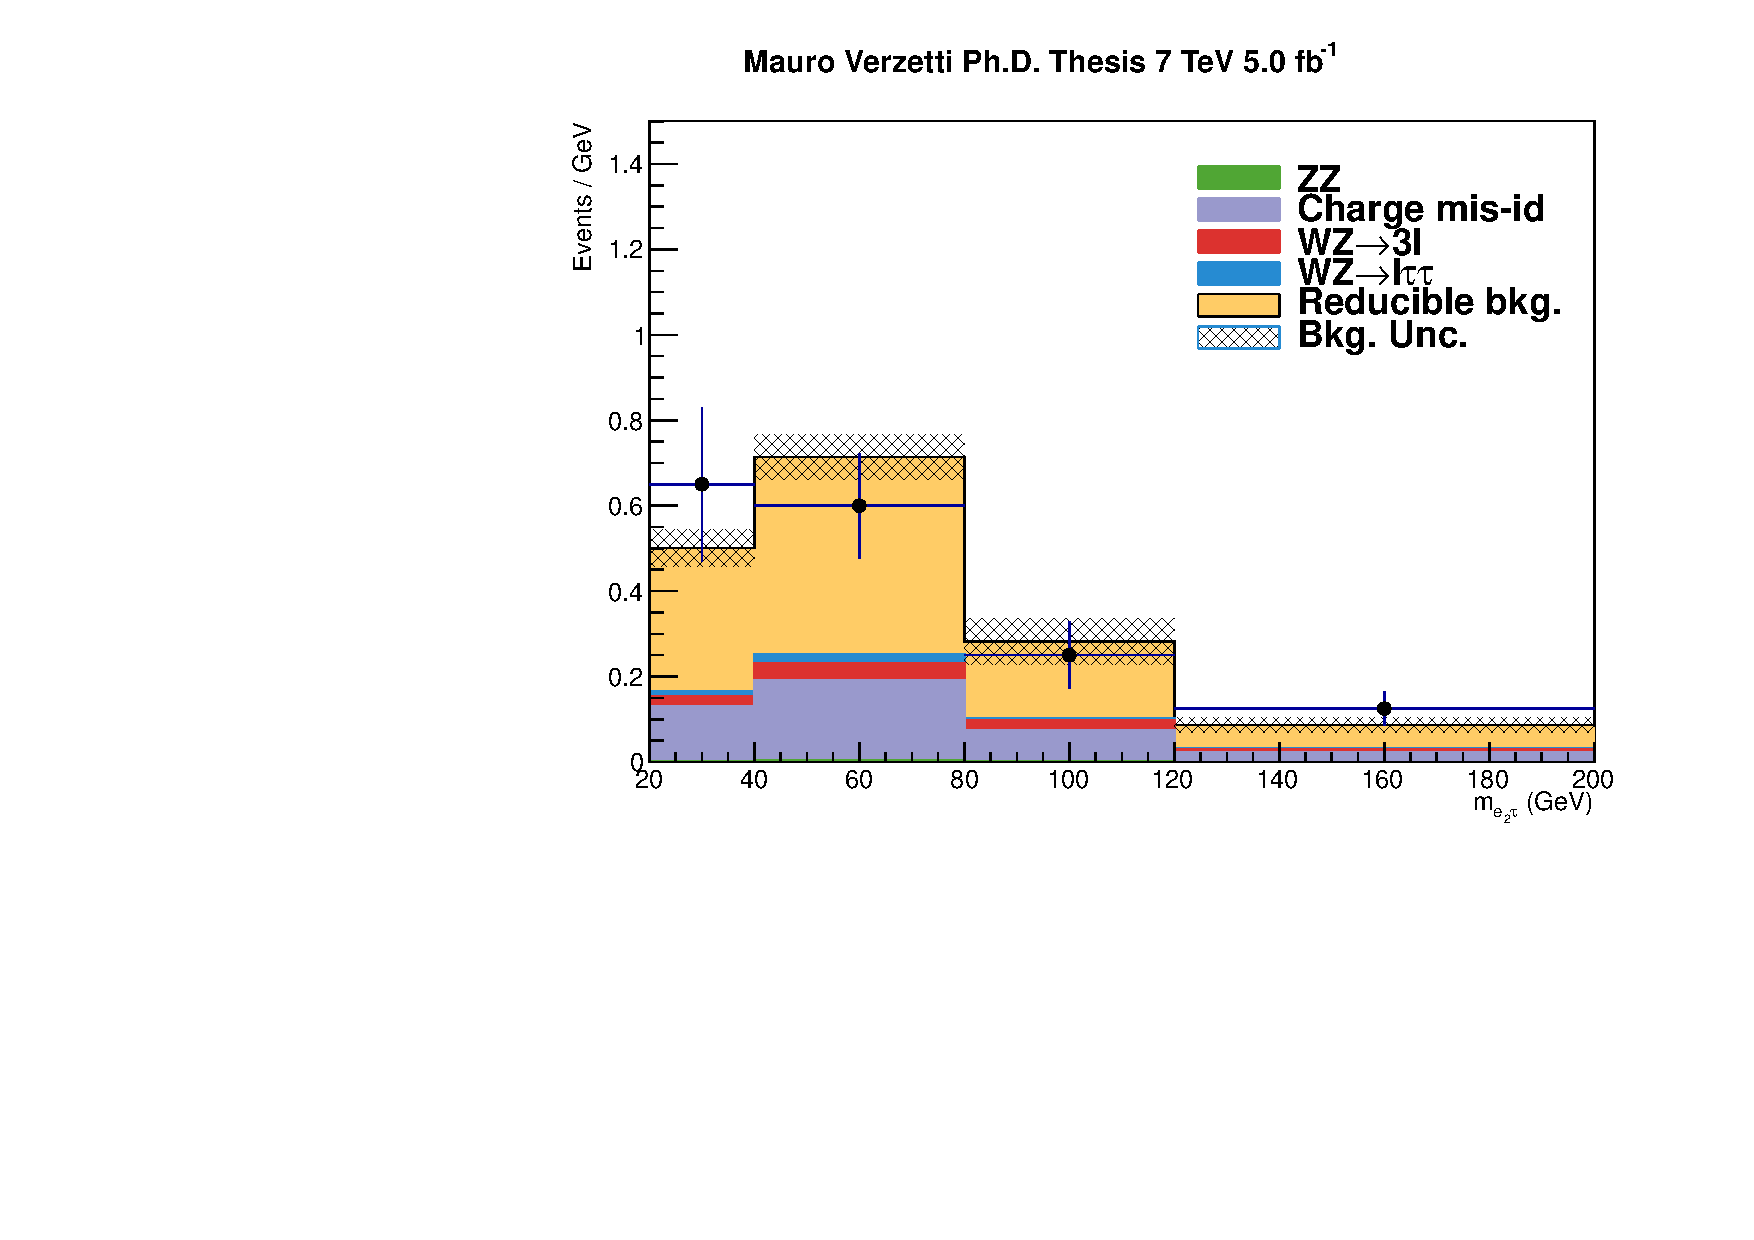
\includegraphics[width=0.49\textwidth]{4_Analisys/pics/7TeV/plots/eet/f3/Full/final-f3-subMass-Full.pdf}
  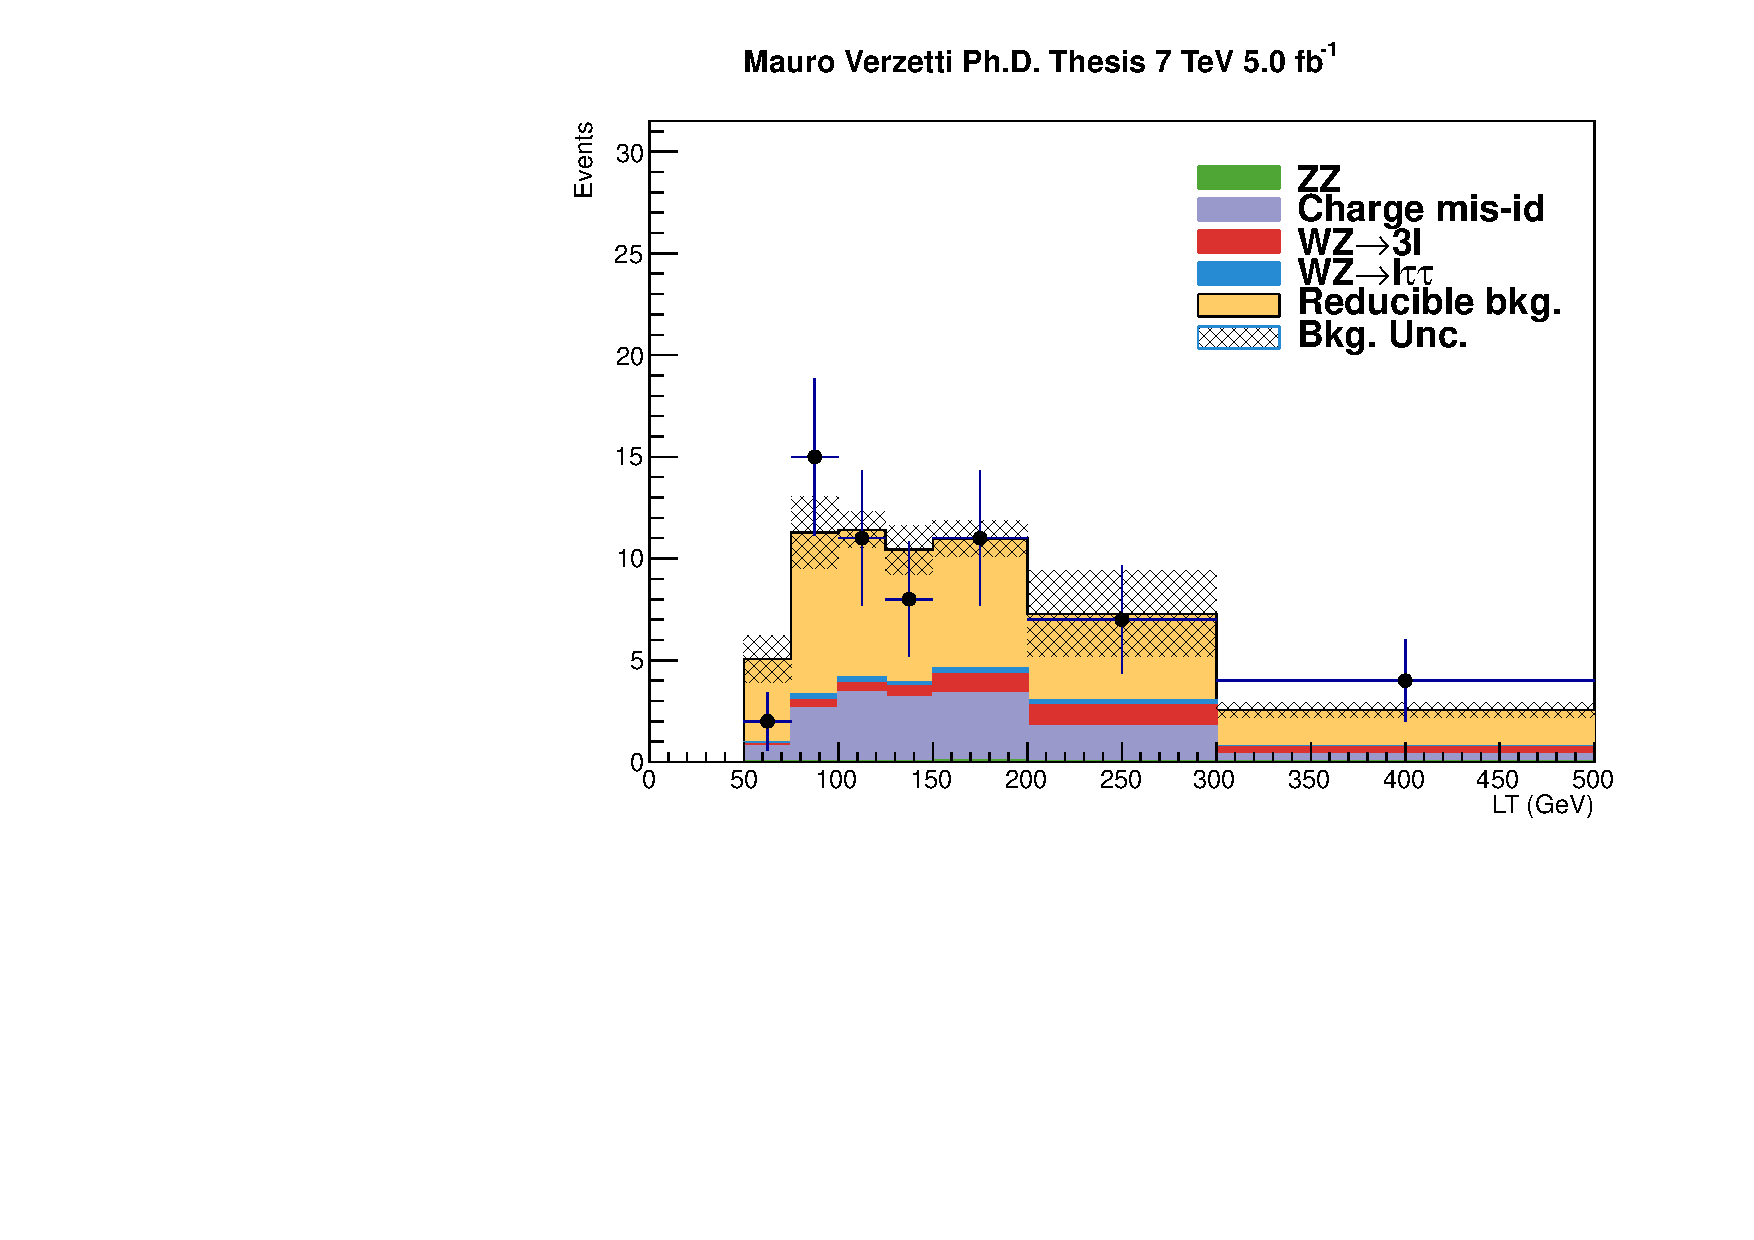
\includegraphics[width=0.49\textwidth]{4_Analisys/pics/7TeV/plots/eet/f3/final-f3-LT.pdf}\\
  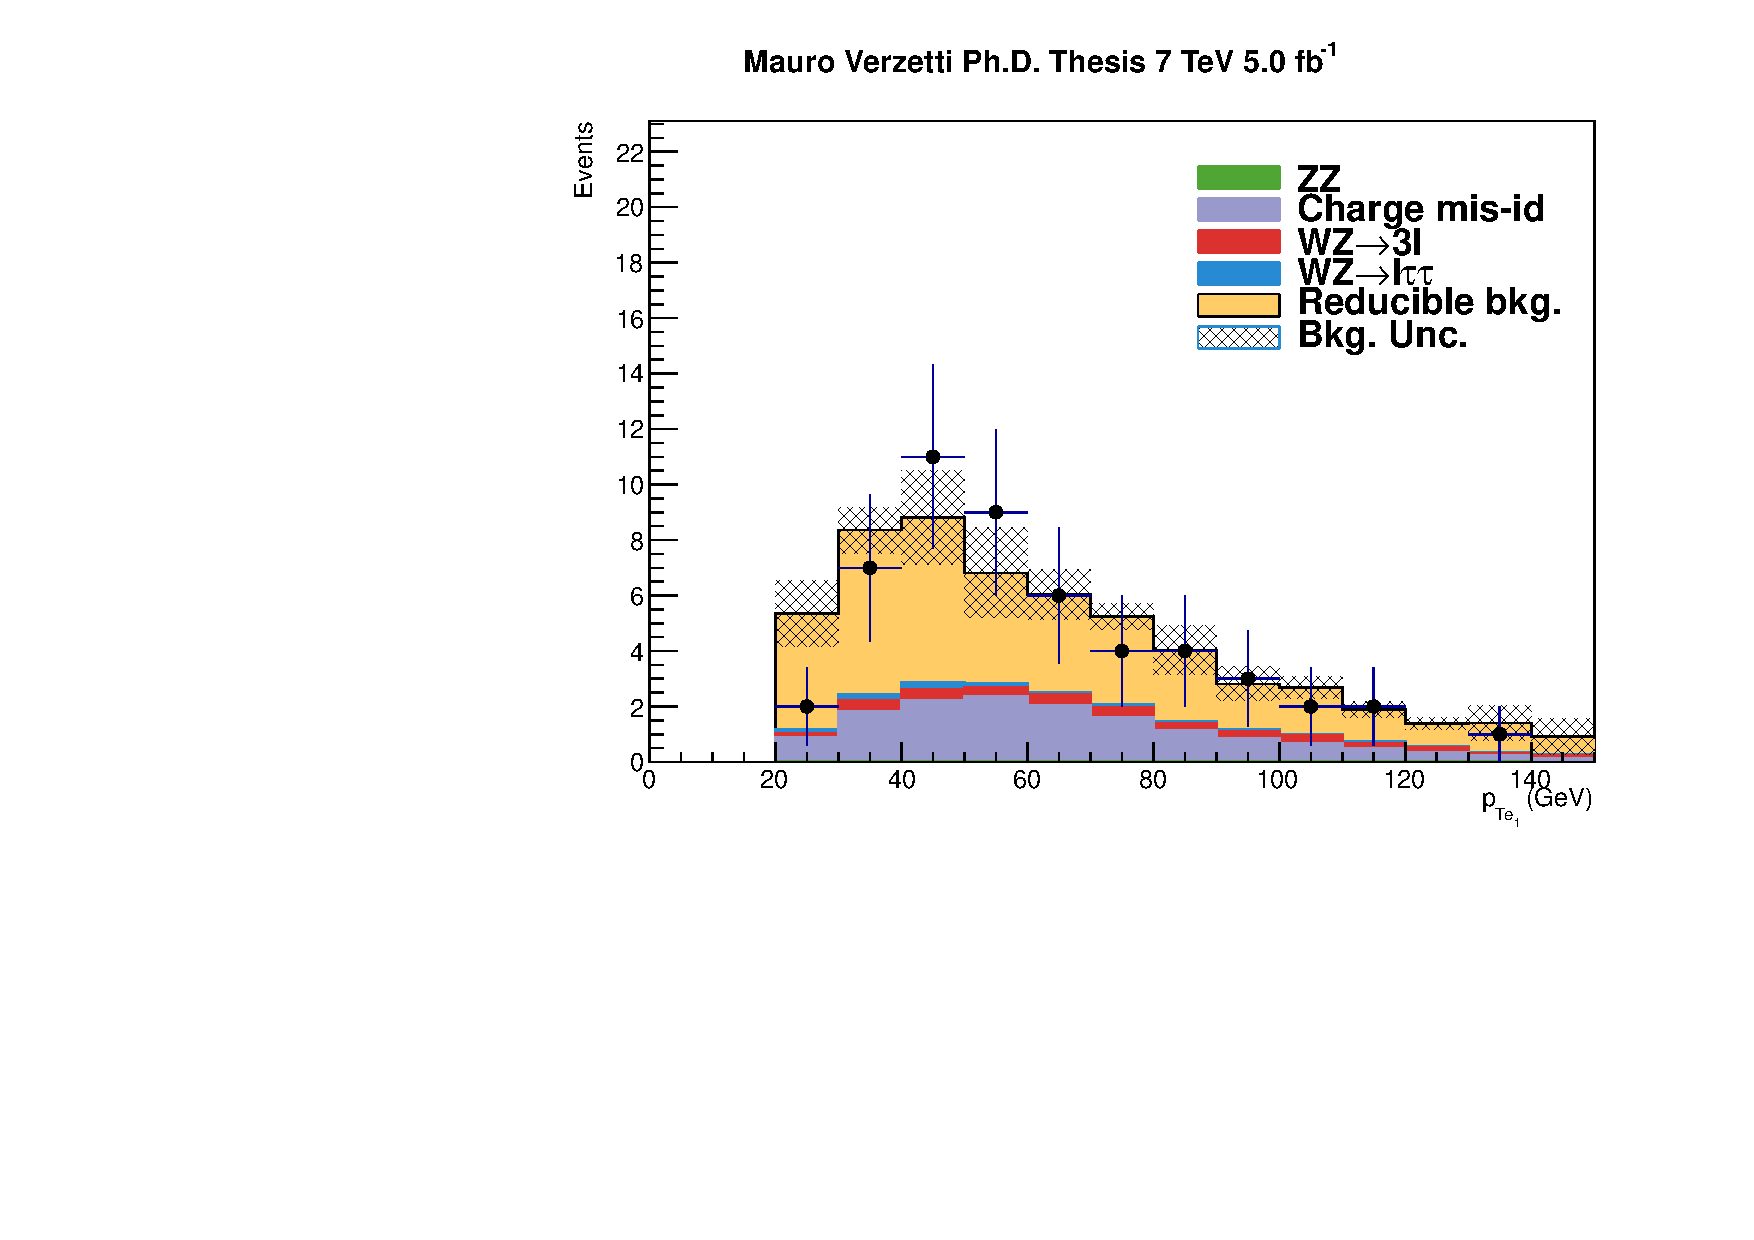
\includegraphics[width=0.49\textwidth]{4_Analisys/pics/7TeV/plots/eet/f3/Full/final-f3-e1Pt-Full.pdf}
  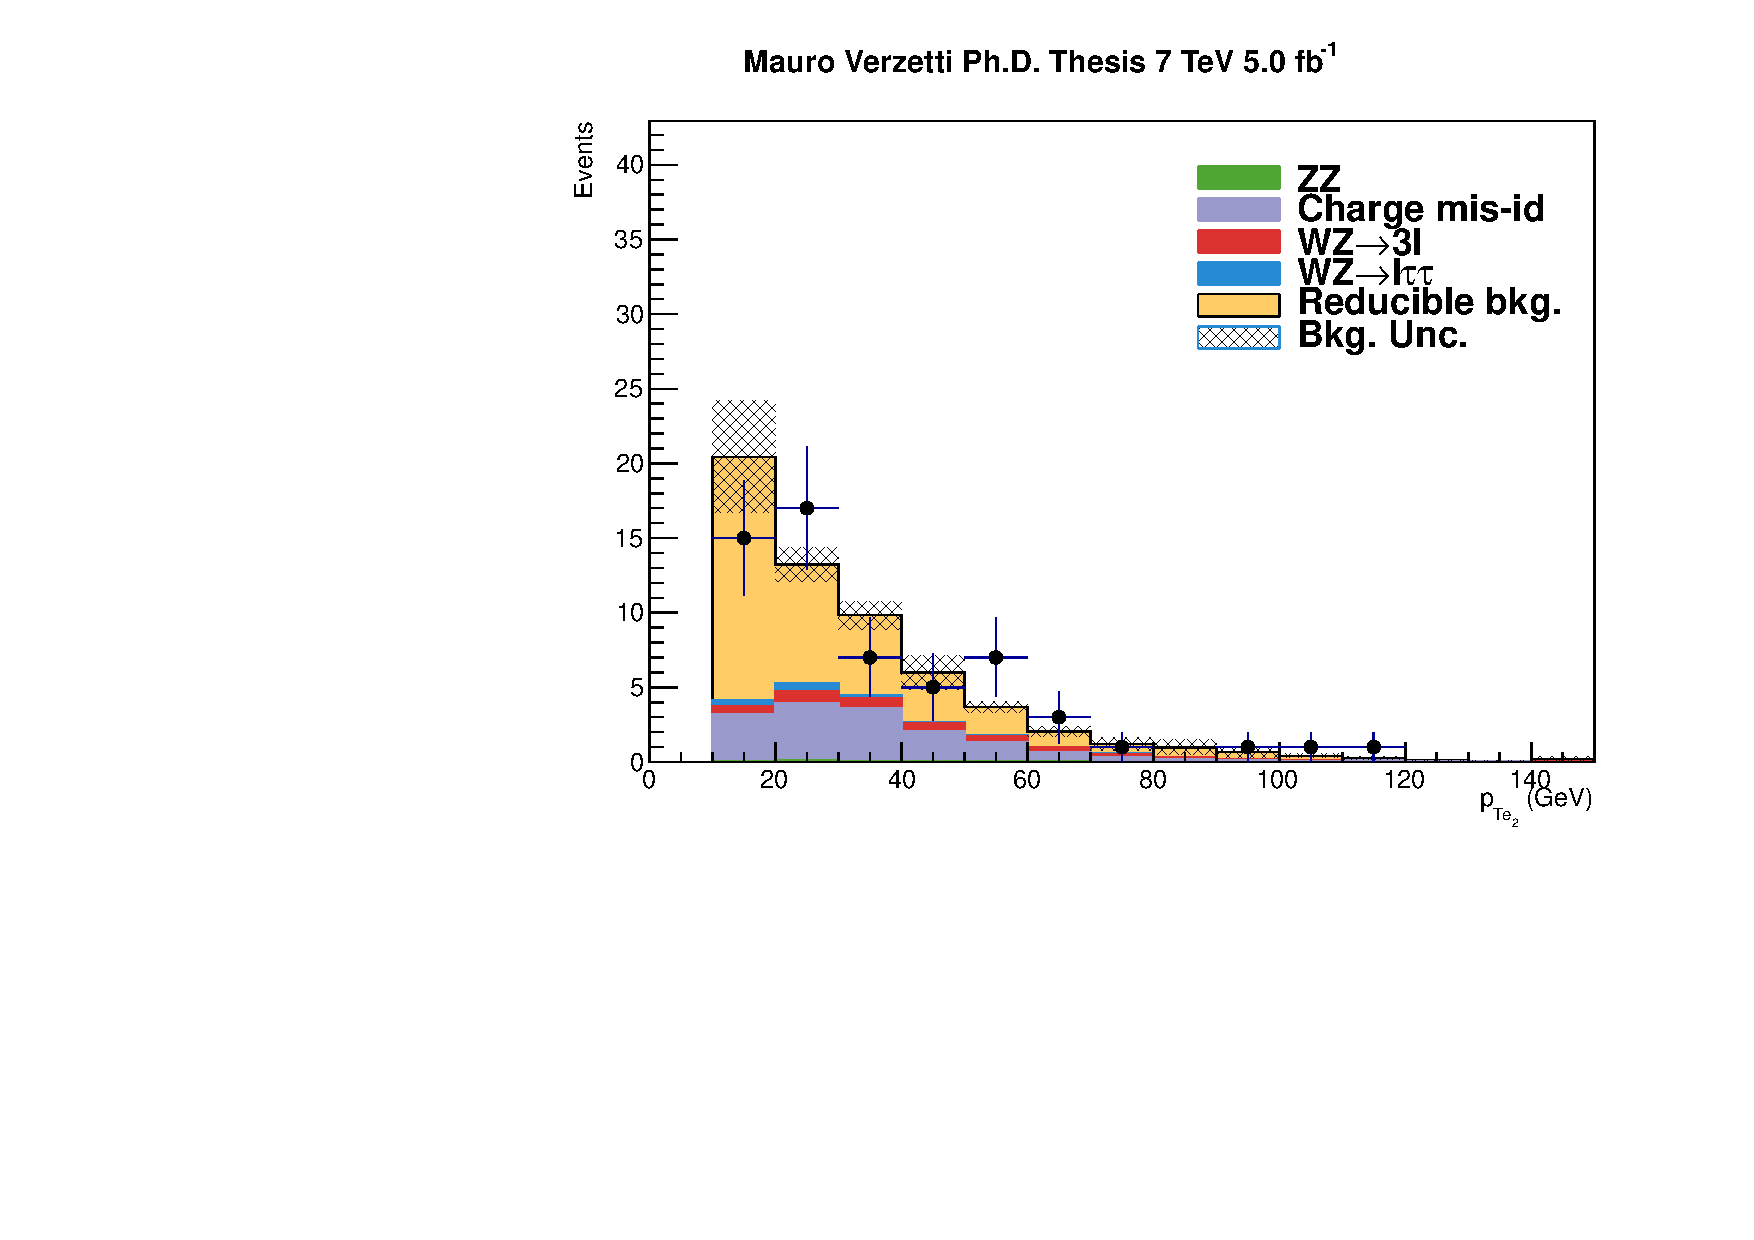
\includegraphics[width=0.49\textwidth]{4_Analisys/pics/7TeV/plots/eet/f3/Full/final-f3-e2Pt-Full.pdf}\\
  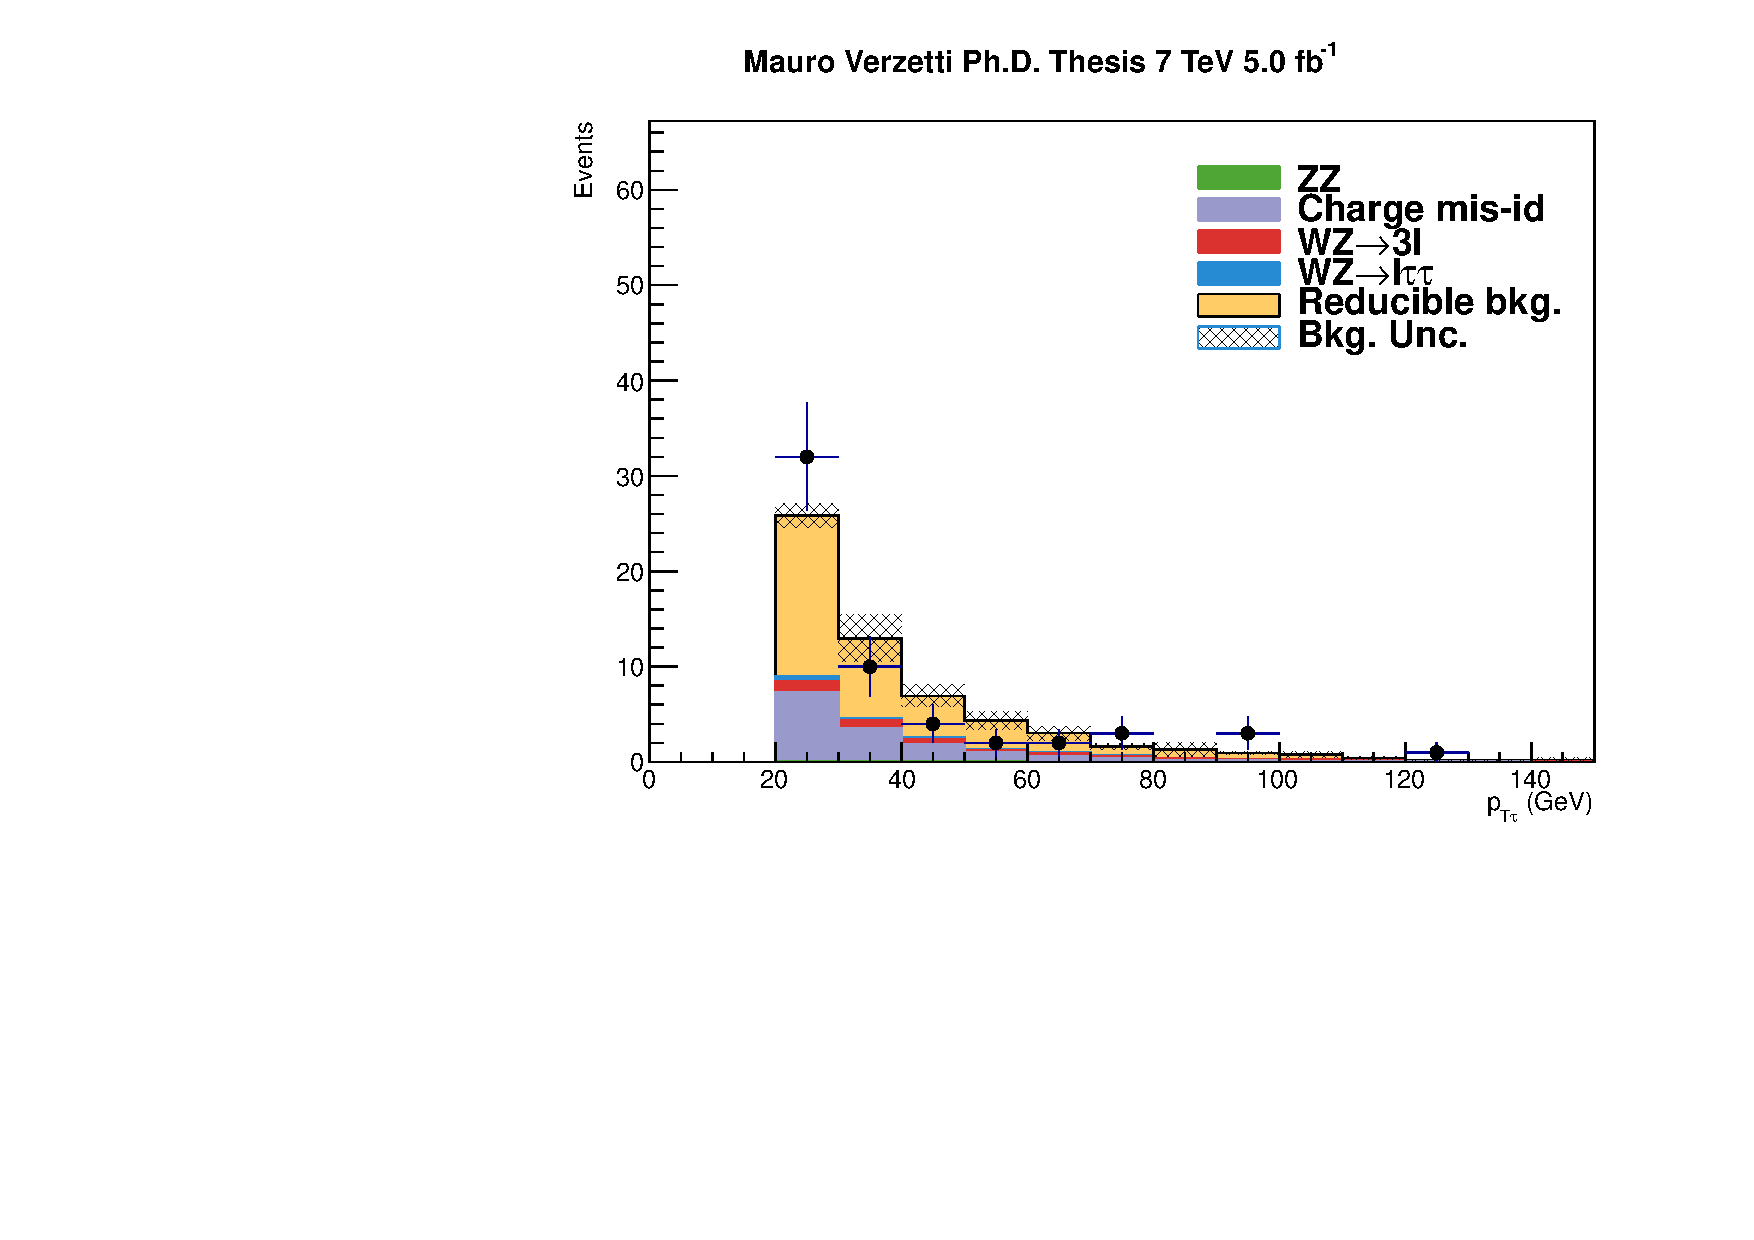
\includegraphics[width=0.49\textwidth]{4_Analisys/pics/7TeV/plots/eet/f3/Full/final-f3-tPt-Full.pdf}
  \caption{Comparison of measured and predicted backgrounds in the $ee\tau_h$ ``fake tau'' control region for 7 TeV data.
  From top left to bottom: mass of the sub-leading electron and the tau system, scalar sum of the leptons \pT ($L_T$), \pT of the leading and sub-leading electron, and \pT of the hadronic tau.
  The reducible background contribution is estimated by the kNN method, as in the signal region.
  The shaded band represents the uncertainty on the sum of the background contributions.
  }
  \label{fig:LLT_eet_f3_control_7TeV}
\end{center}
\end{figure}

\begin{figure}
\begin{center}
  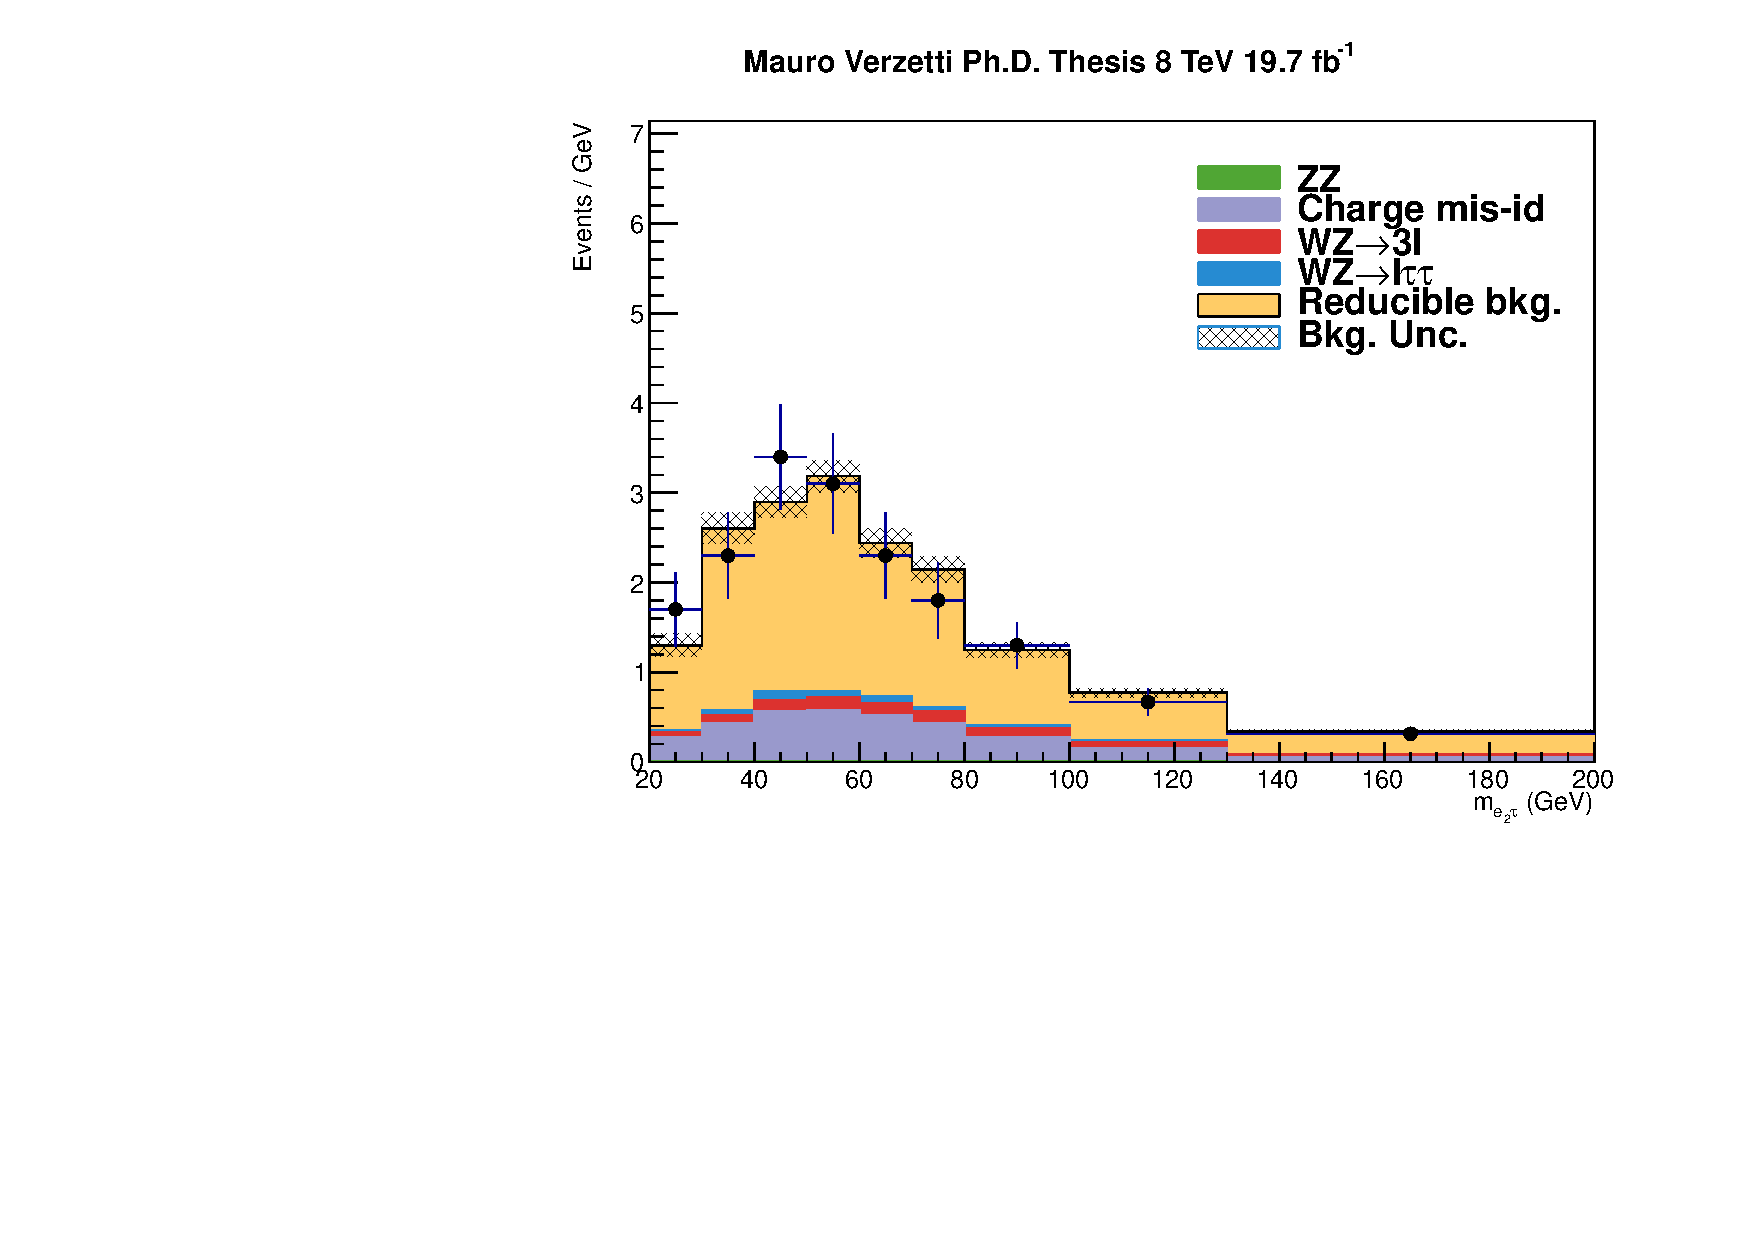
\includegraphics[width=0.49\textwidth]{4_Analisys/pics/8TeV/plots/eet/f3/Full/final-f3-subMass-Full.pdf}
  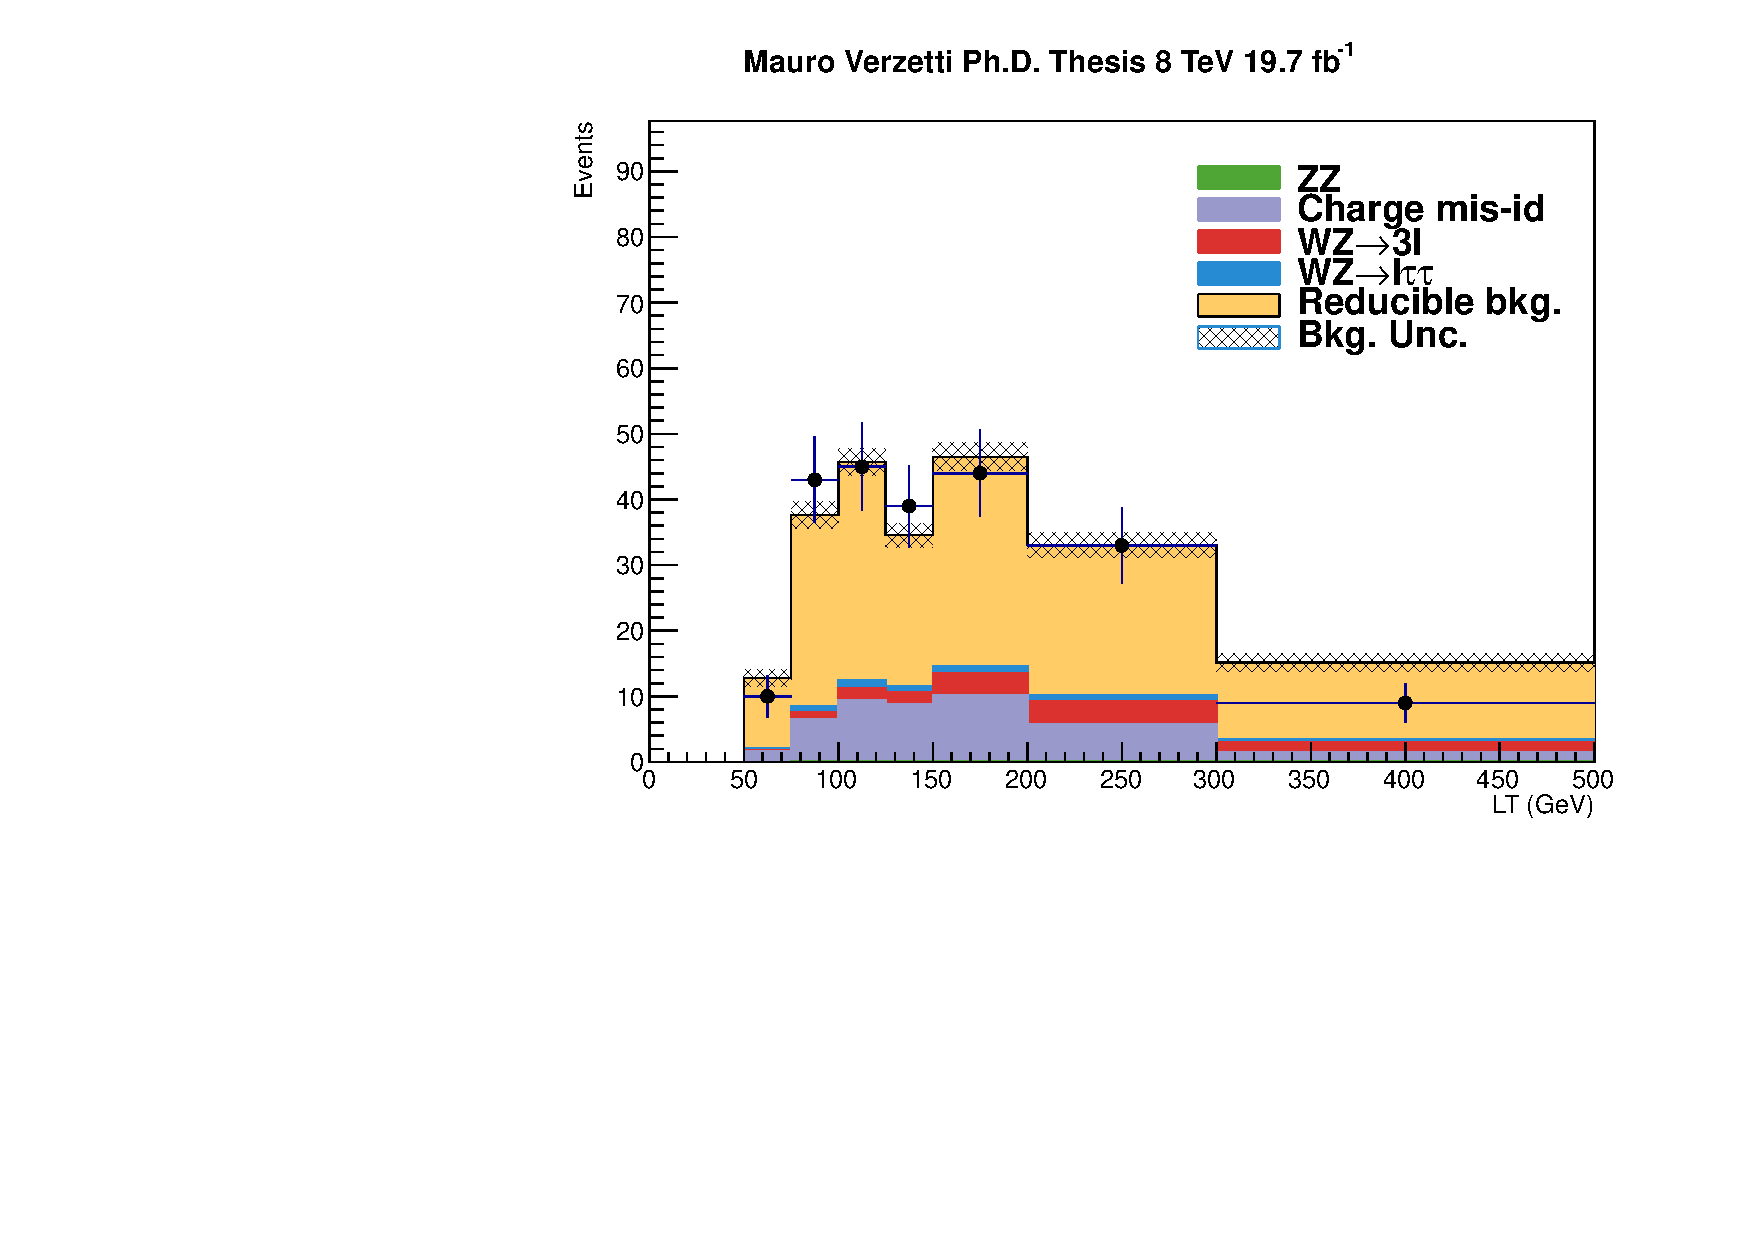
\includegraphics[width=0.49\textwidth]{4_Analisys/pics/8TeV/plots/eet/f3/final-f3-LT.pdf}\\
  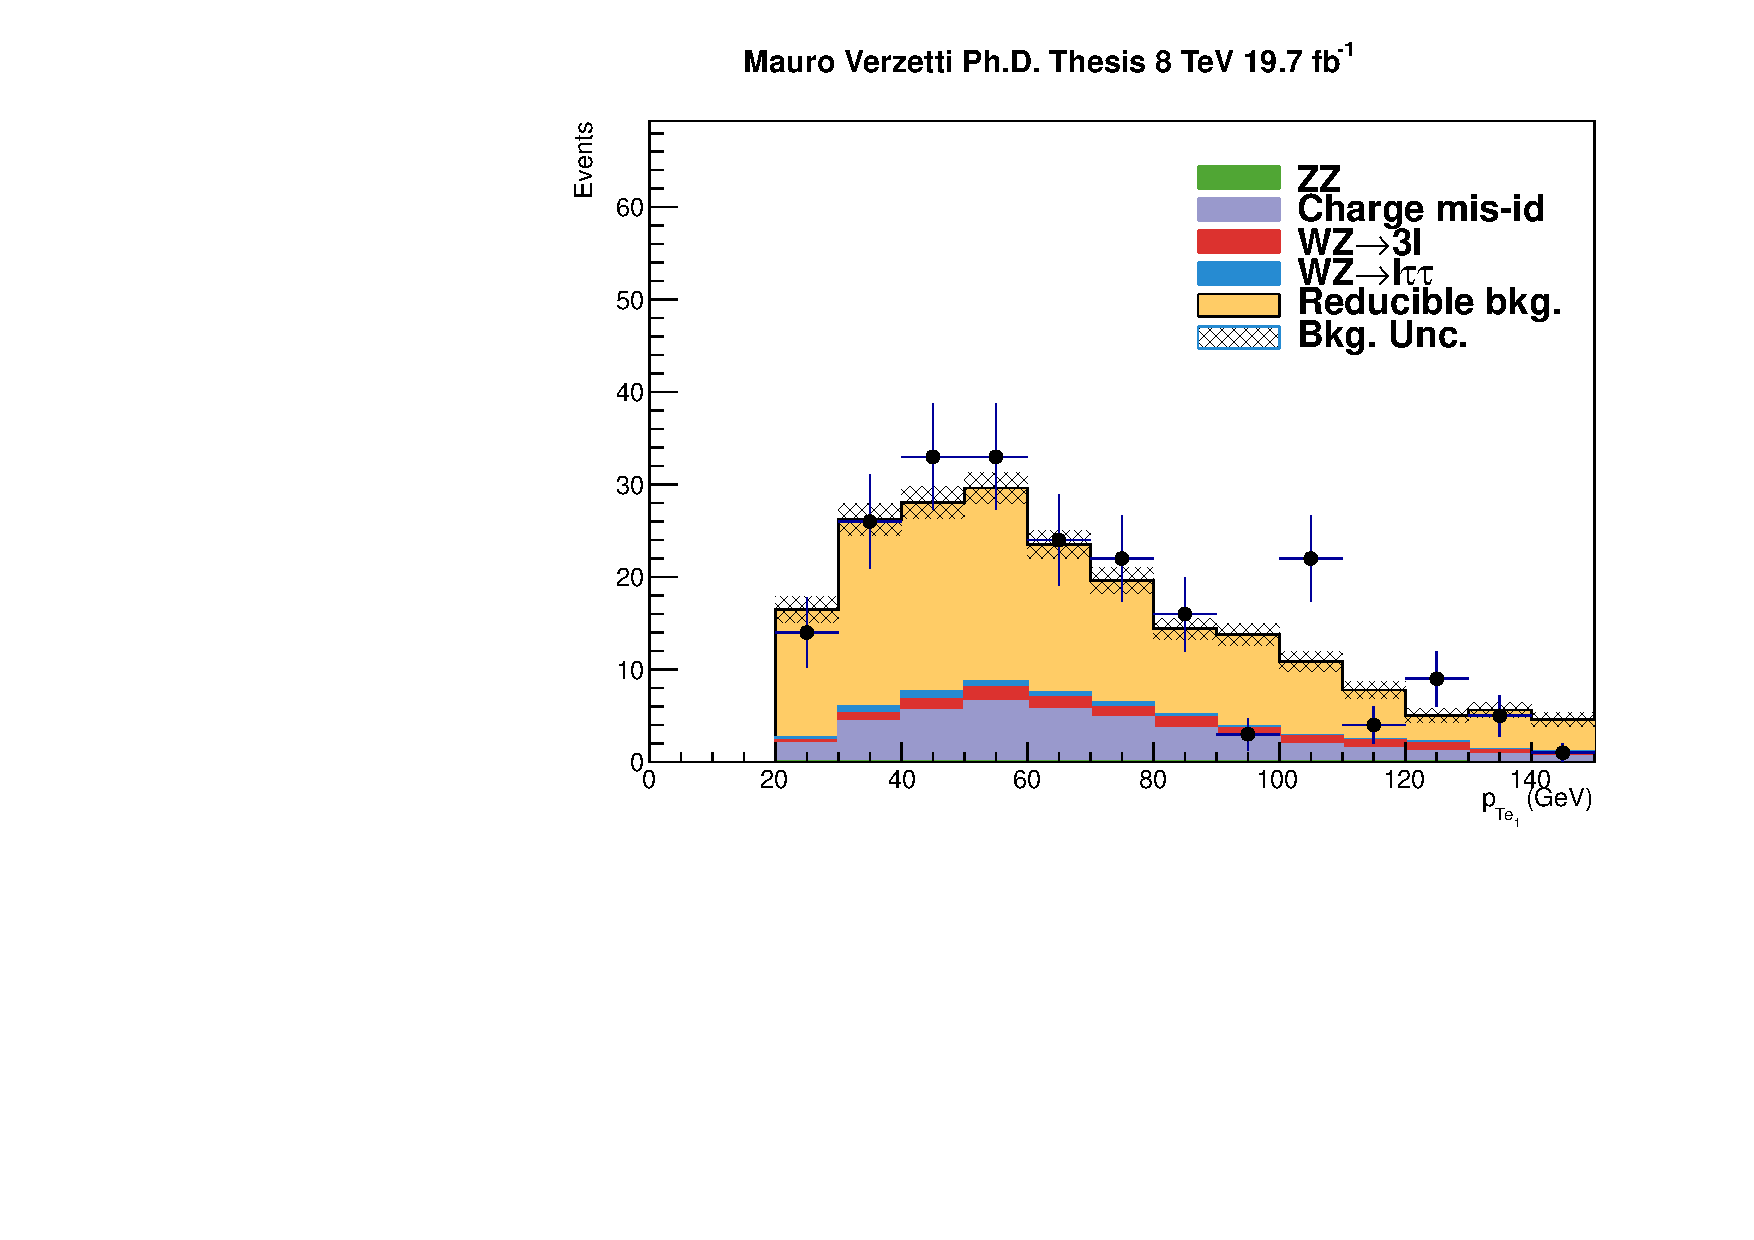
\includegraphics[width=0.49\textwidth]{4_Analisys/pics/8TeV/plots/eet/f3/Full/final-f3-e1Pt-Full.pdf}
  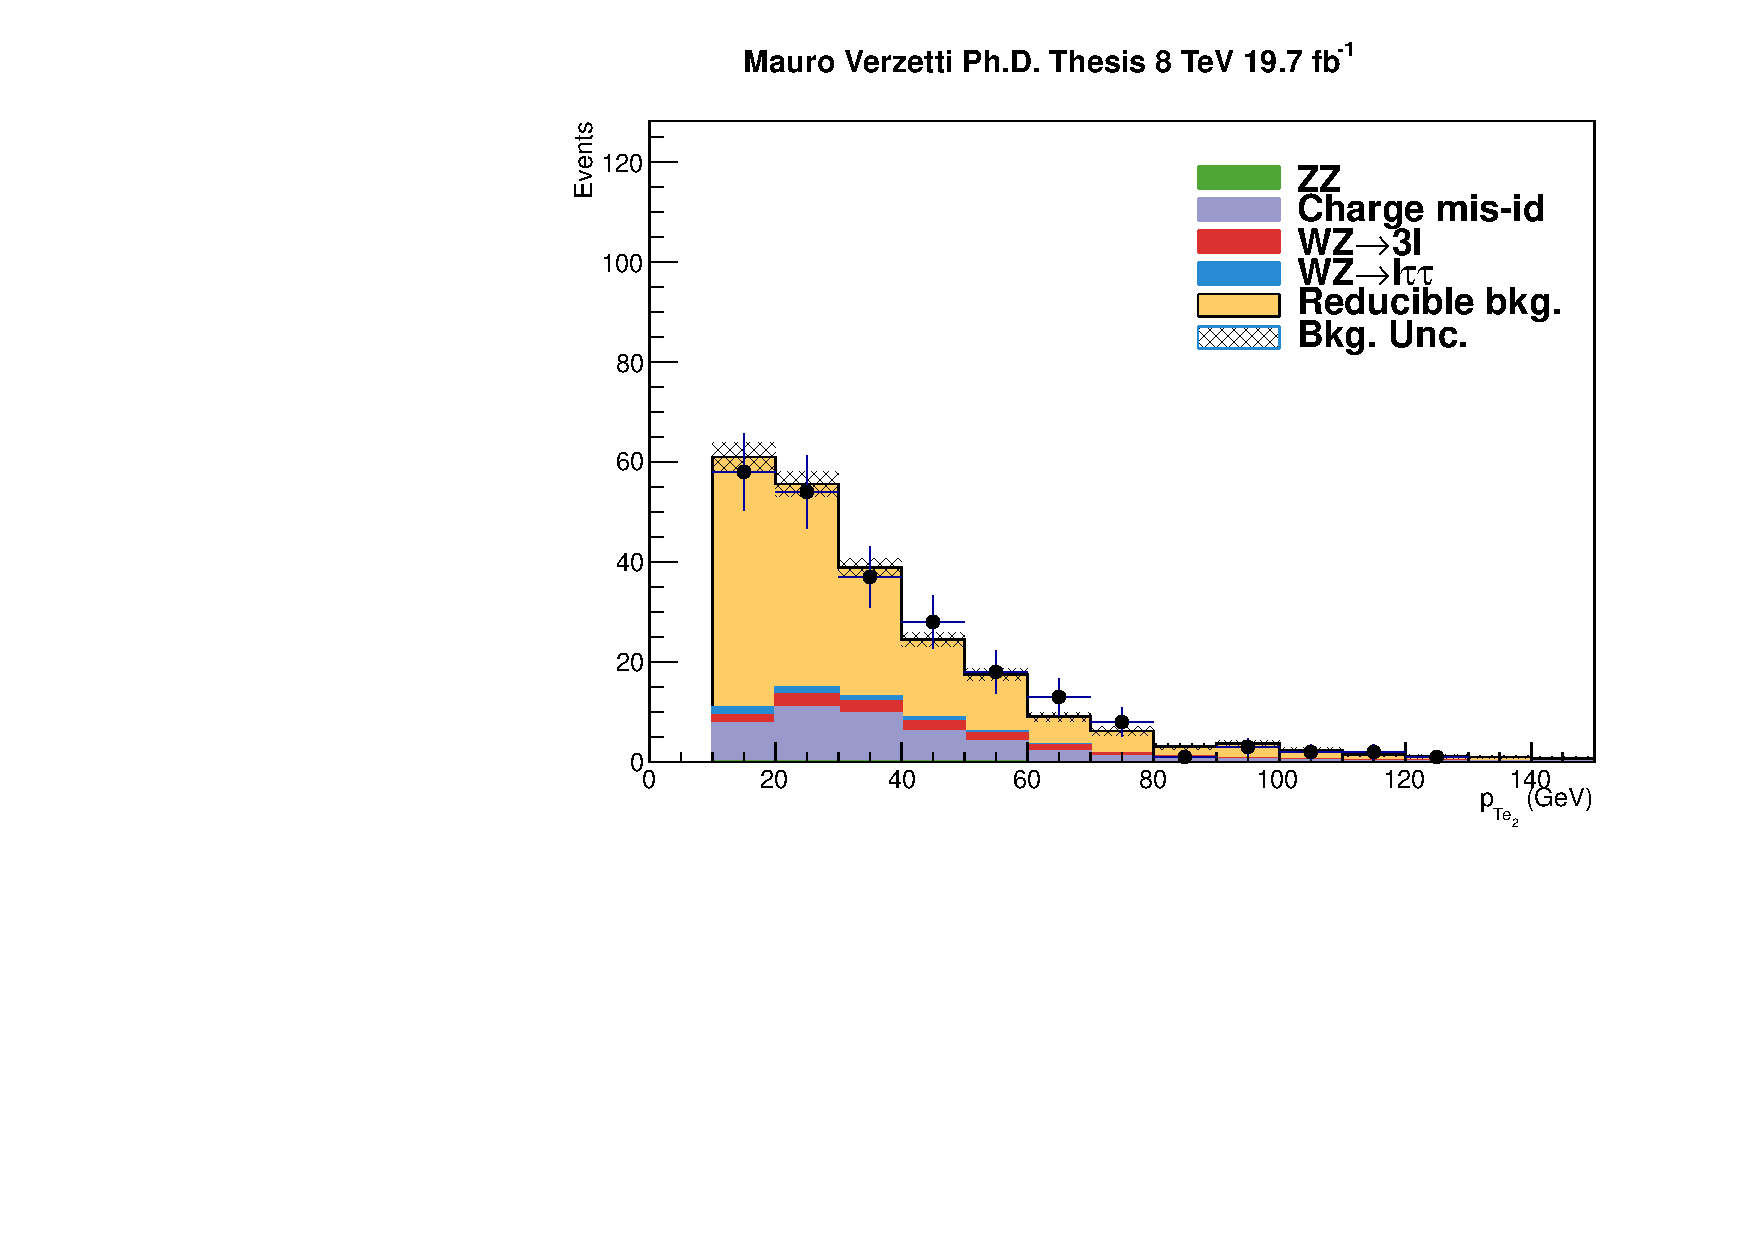
\includegraphics[width=0.49\textwidth]{4_Analisys/pics/8TeV/plots/eet/f3/Full/final-f3-e2Pt-Full.pdf}\\
  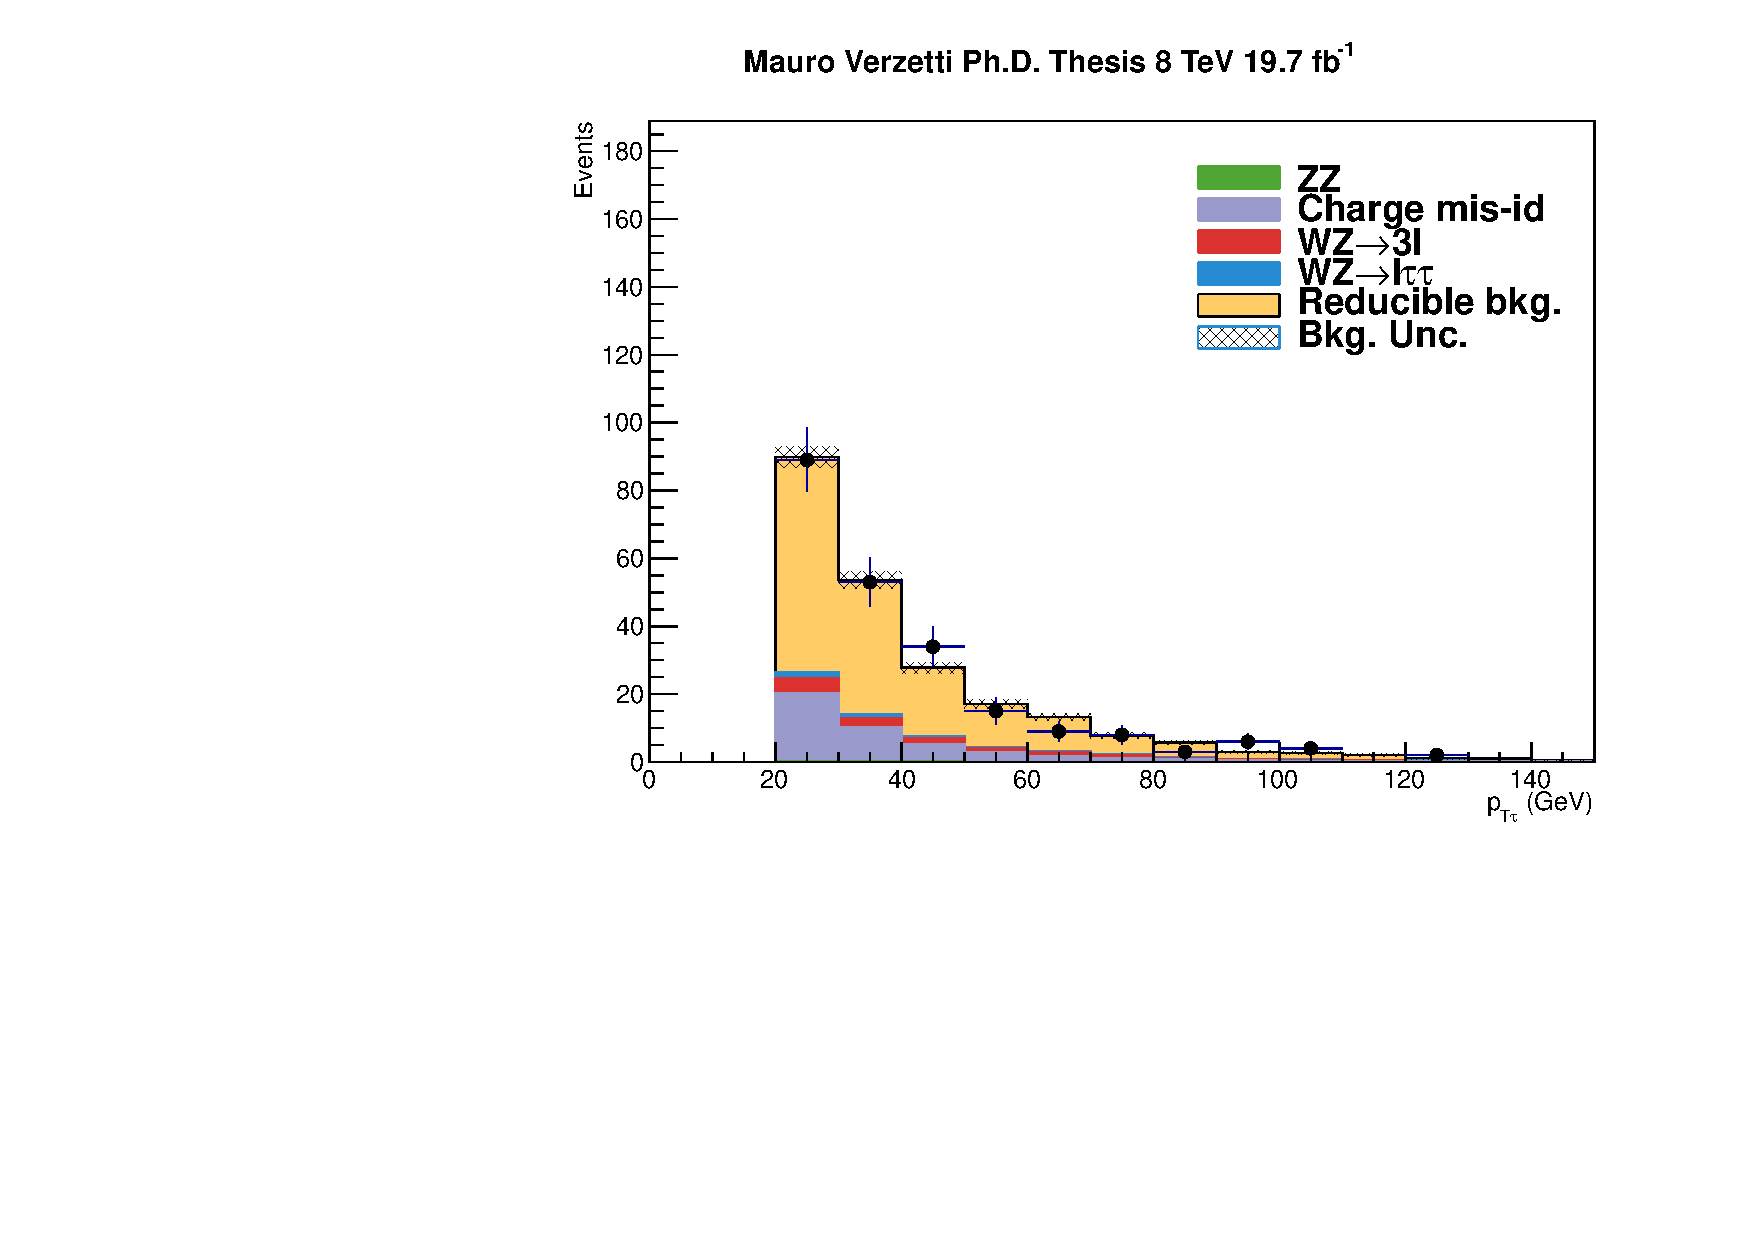
\includegraphics[width=0.49\textwidth]{4_Analisys/pics/8TeV/plots/eet/f3/Full/final-f3-tPt-Full.pdf}
  \caption{Comparison of measured and predicted backgrounds in the $ee\tau_h$ ``fake tau'' control region for 8 TeV data.
  From top left to bottom: mass of the sub-leading electron and the tau system, scalar sum of the leptons \pT ($L_T$), \pT of the leading and sub-leading electron, and \pT of the hadronic tau.
  The reducible background contribution is estimated by the kNN method, as in the signal region.
  The shaded band represents the uncertainty on the sum of the background contributions.
  }
  \label{fig:LLT_eet_f3_control_8TeV}
\end{center}
\end{figure}

\subsection{Fake tau method}

To better estimate the solidity of the the ``fake lepton'' method against differences in composition of the training sample and the sample to which the method is applied, a second background estimate is performed.
This methodology is very similar to the previous one, but the object considered as possibly mis-reconstructed is the hadronic tau.

\subsubsection{Region definition}

The misidentification probability for $\tau_h$ candidates is measured in $W+$Jets events, requiring:
\begin{itemize}
\item Events must pass the single muon trigger;
\item A muon candidate with $\pt > 24$ GeV and $|\eta| < 2.1$;
\item The muon must pass the tight Particle Flow identification and have a combined PF Relative Isolation $\Delta \beta $ corrected below $0.1$;
\item The longitudinal impact parameter of the muon track with respect to the primary vertex must be less than 0.2 cm;
\item $m_{T}(\mu, \met) > 40\GeV$;
\item Two same sign tau candidates are required, both with opposite charge to the muon;
\item Events are rejected if they contain another muon or electron with $\pt > 15$ GeV;
\item Events are rejected if they contain a jet with $\pt > 20$ GeV and $|\eta|< 2.4$ satisfying the loose CSV b--tagging working point.
\end{itemize}
The tau fake-rate is measured individually for the 2011 and 2012 run periods in three regions of pseudo-rapidity ($|\eta|<0.8$,
\mbox{$0.8<|\eta|<1.6$} and $1.6<|\eta|<2.3$) and as a function of the tau \pT. The chosen fake-rate is modeled by a Landau function. % with peak and width left free to float.%, and an additive constant.
The width and peak parameters are adjusted to best match the measured $\rm{jet}\To\tau_h$ fake-rates.

The fake rates measured in the %measured tau misidentification rates in both 
7 TeV and 8 TeV data are shown in figure~\ref{fig:LLT_tau_FR}. The $\rm{jet}\To\tau_h$ fake-rate %measured tau misidentification rate 
ranges from 6\% at low tau \pT in the end--cap region, to 1\% at high \pT ($ > 80$ GeV) in the central region.

\begin{figure}
  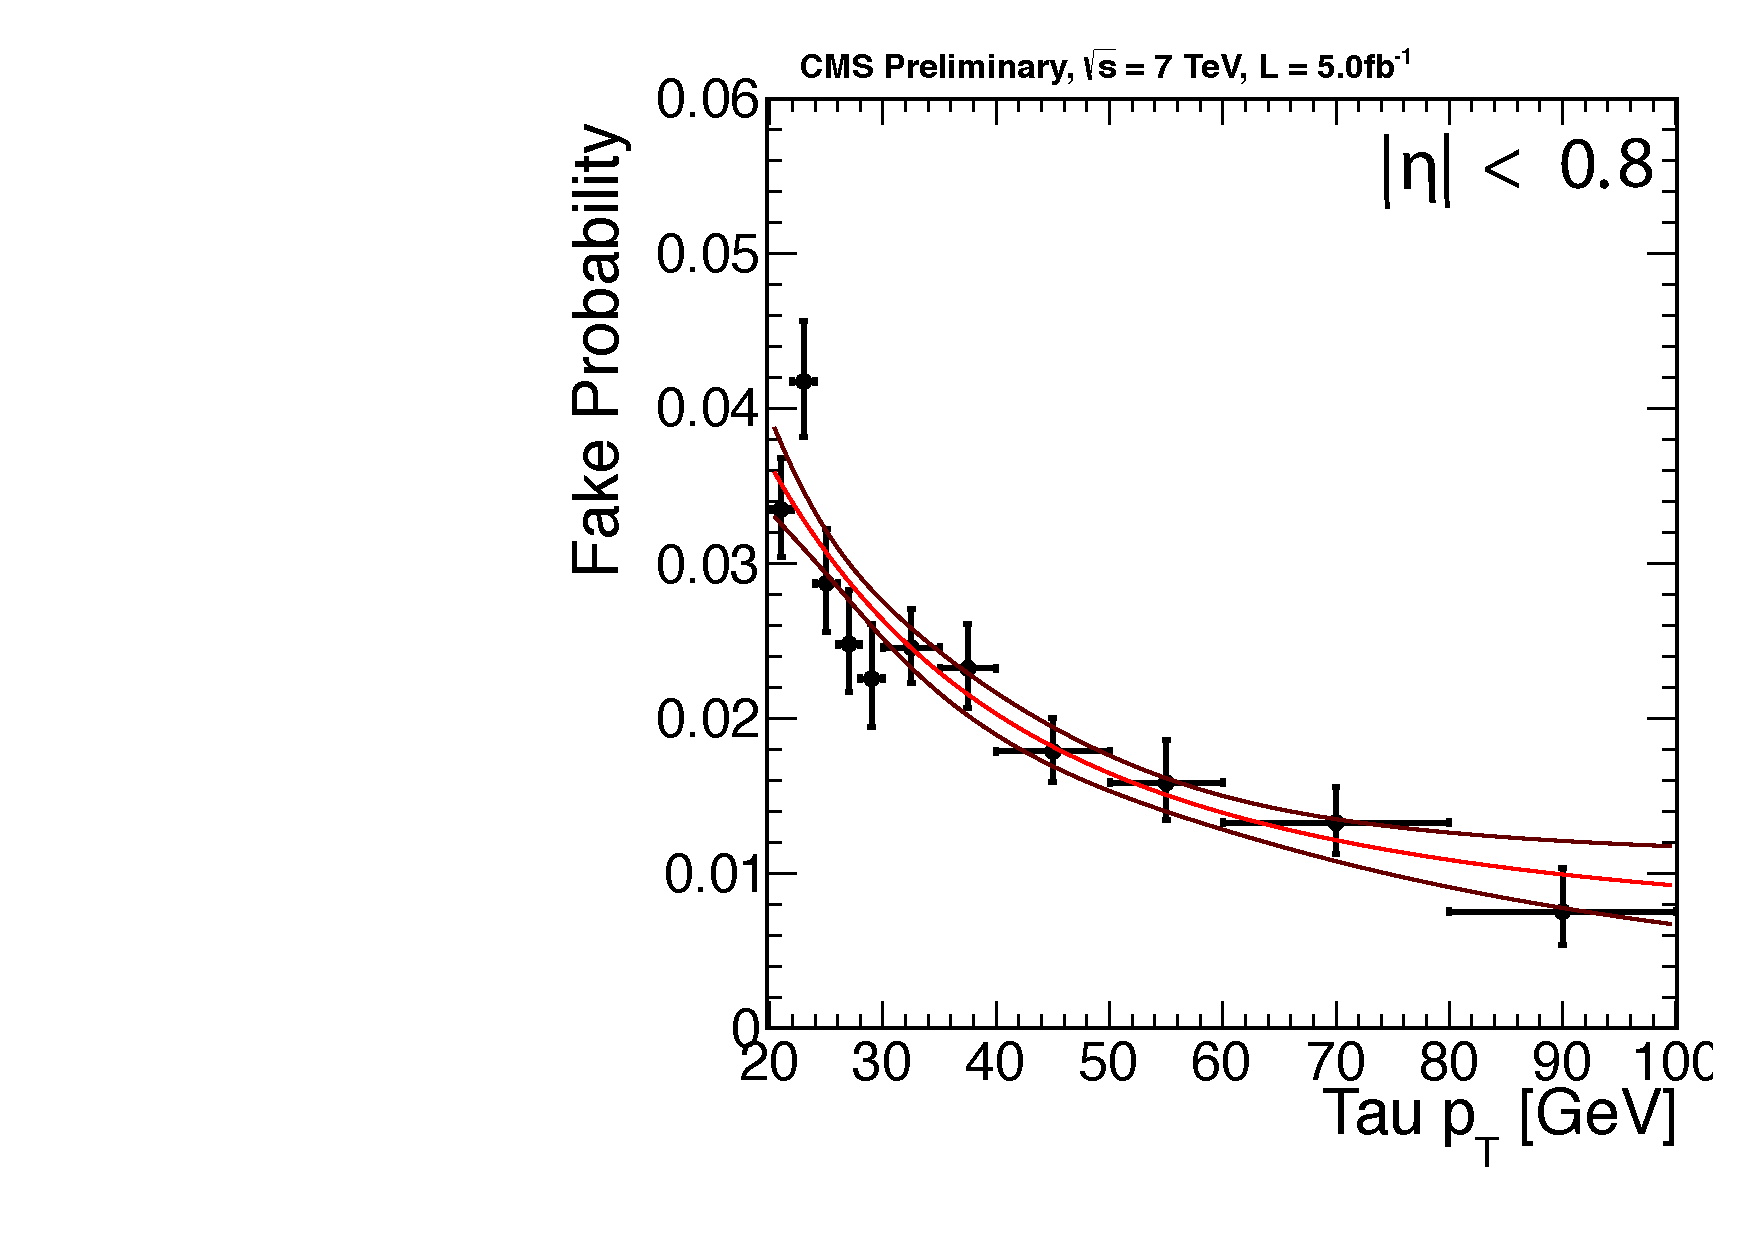
\includegraphics[width=0.33\textwidth]{4_Analisys/pics/7TeV/fakerate_fits/tau_fr_barrel.pdf}
  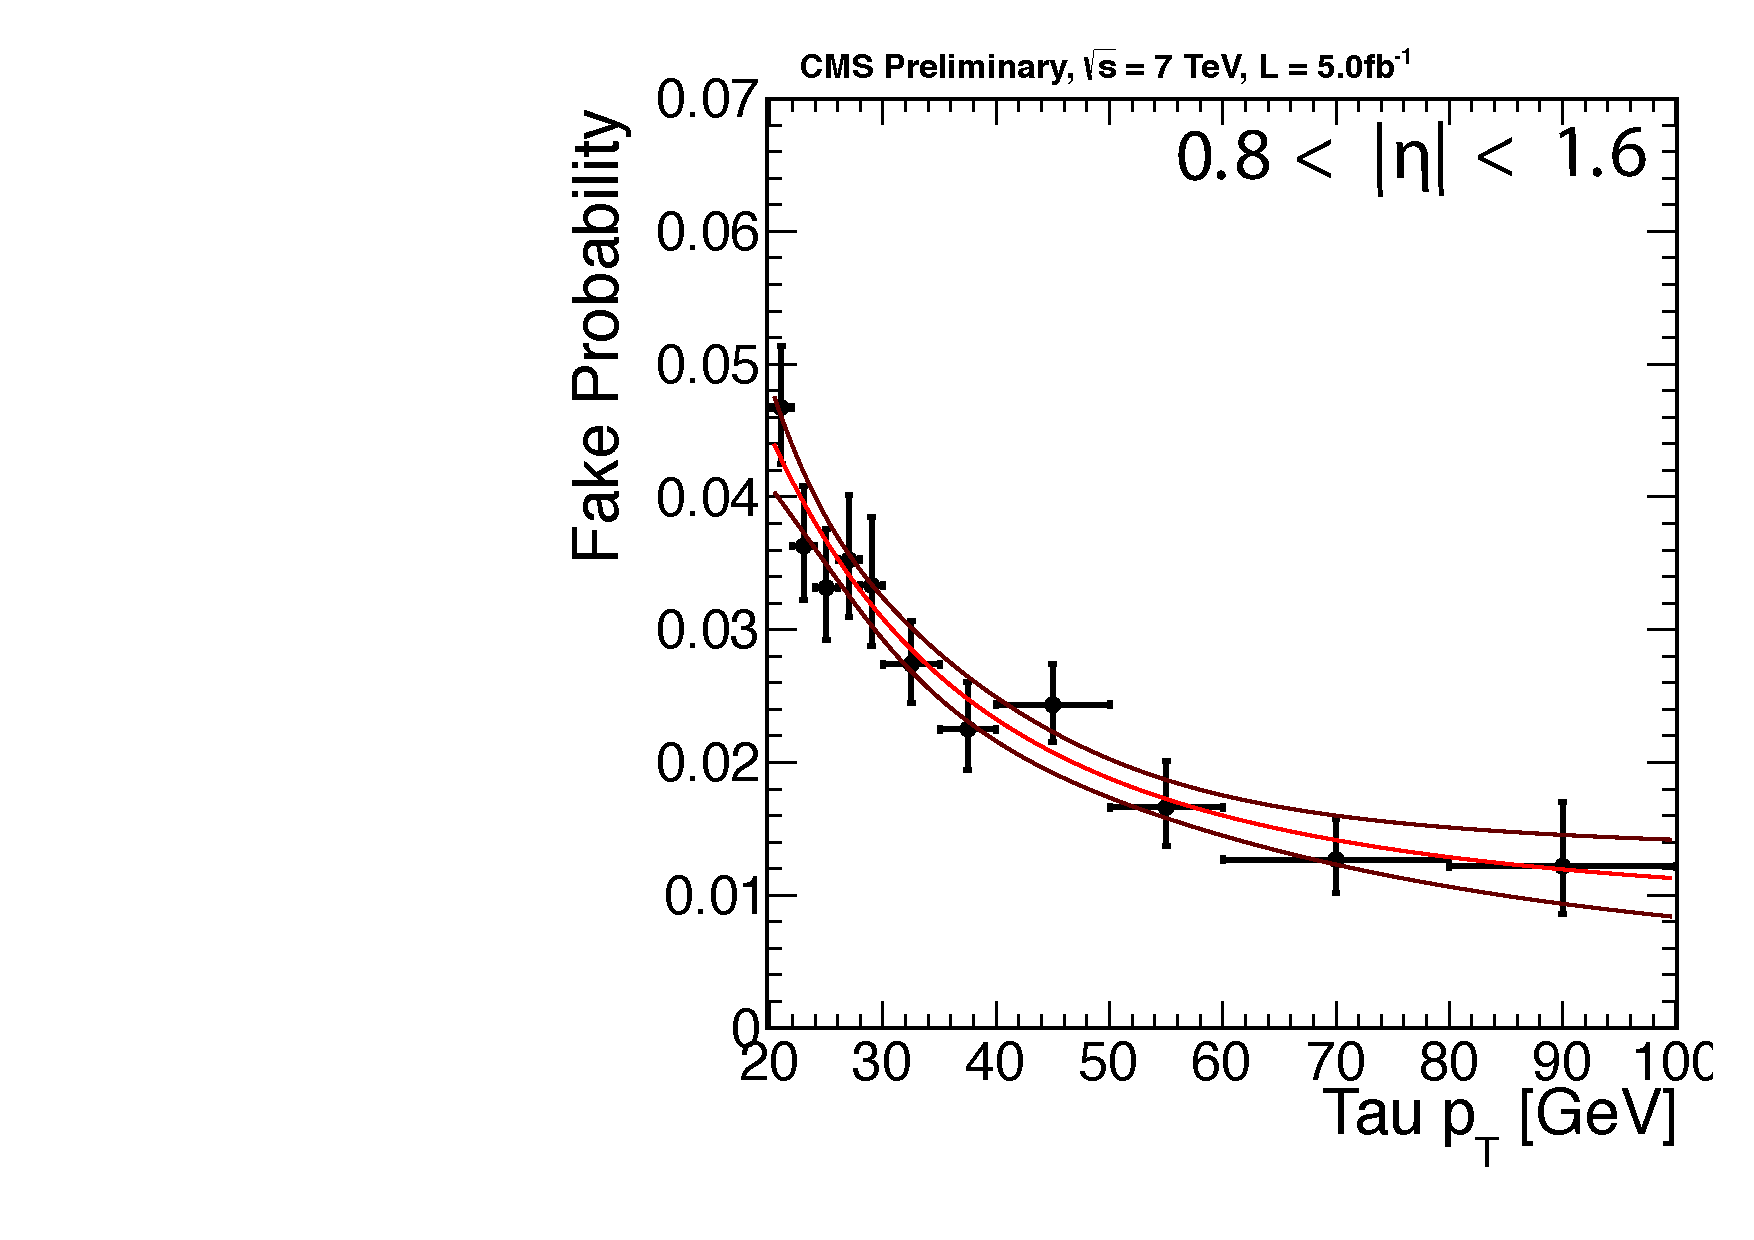
\includegraphics[width=0.33\textwidth]{4_Analisys/pics/7TeV/fakerate_fits/tau_fr_transition.pdf}
  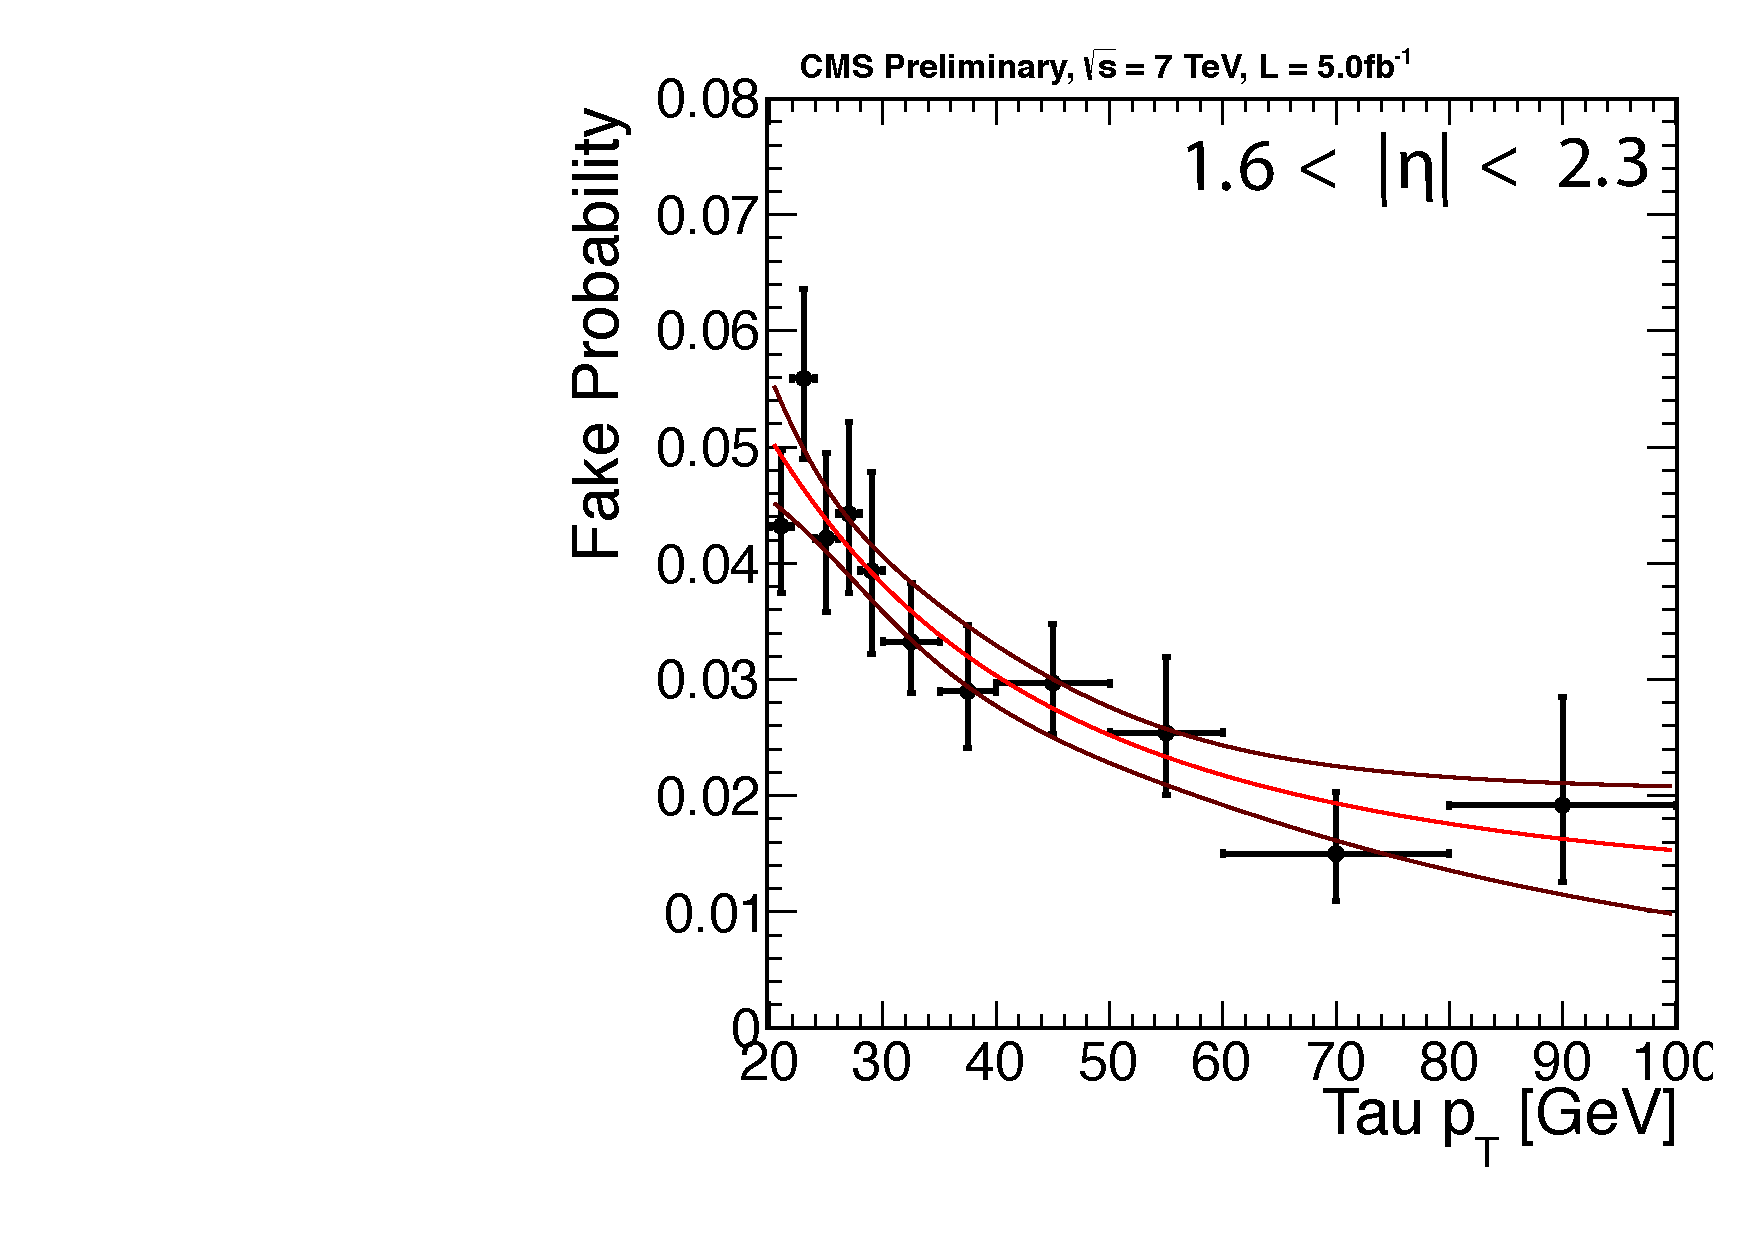
\includegraphics[width=0.33\textwidth]{4_Analisys/pics/7TeV/fakerate_fits/tau_fr_endcap.pdf}\\
  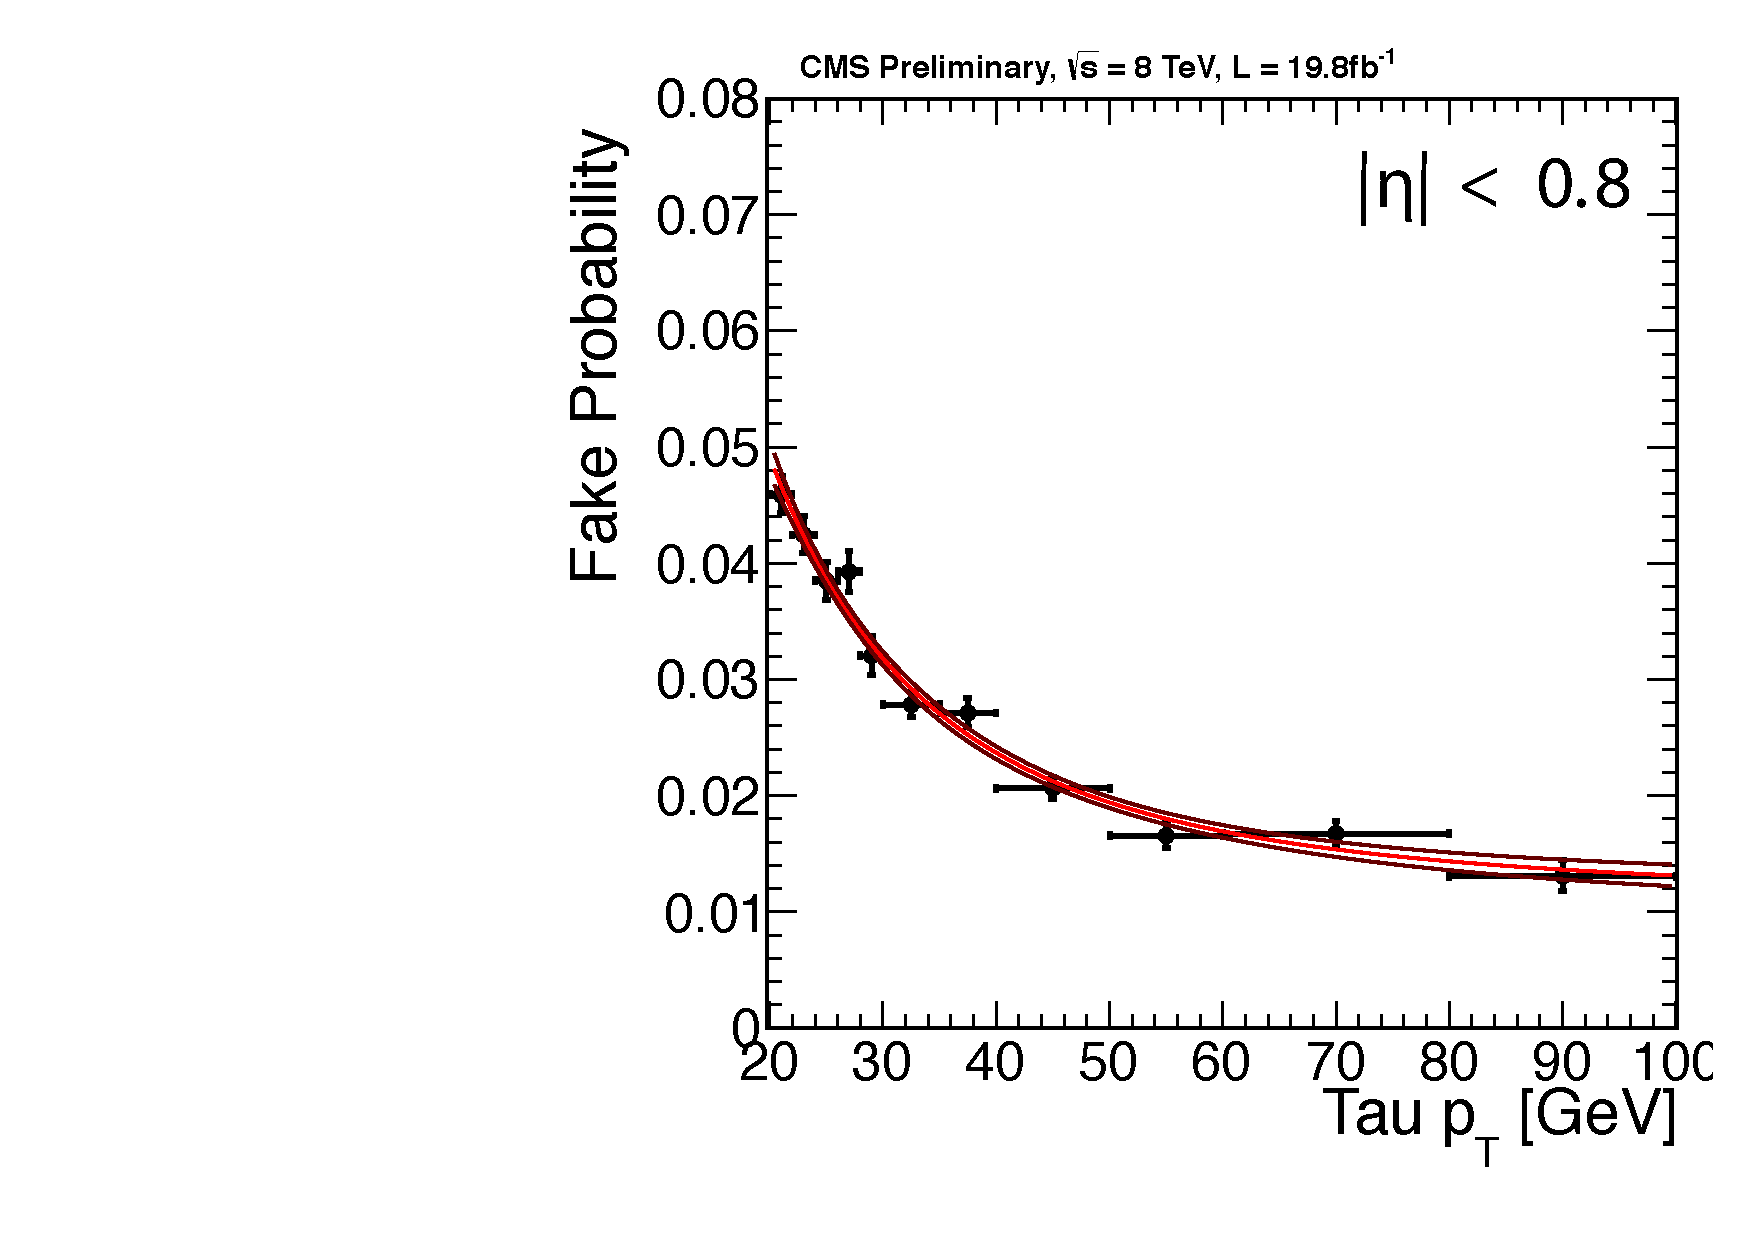
\includegraphics[width=0.33\textwidth]{4_Analisys/pics/8TeV/fakerate_fits/tau_fr_barrel.pdf}
  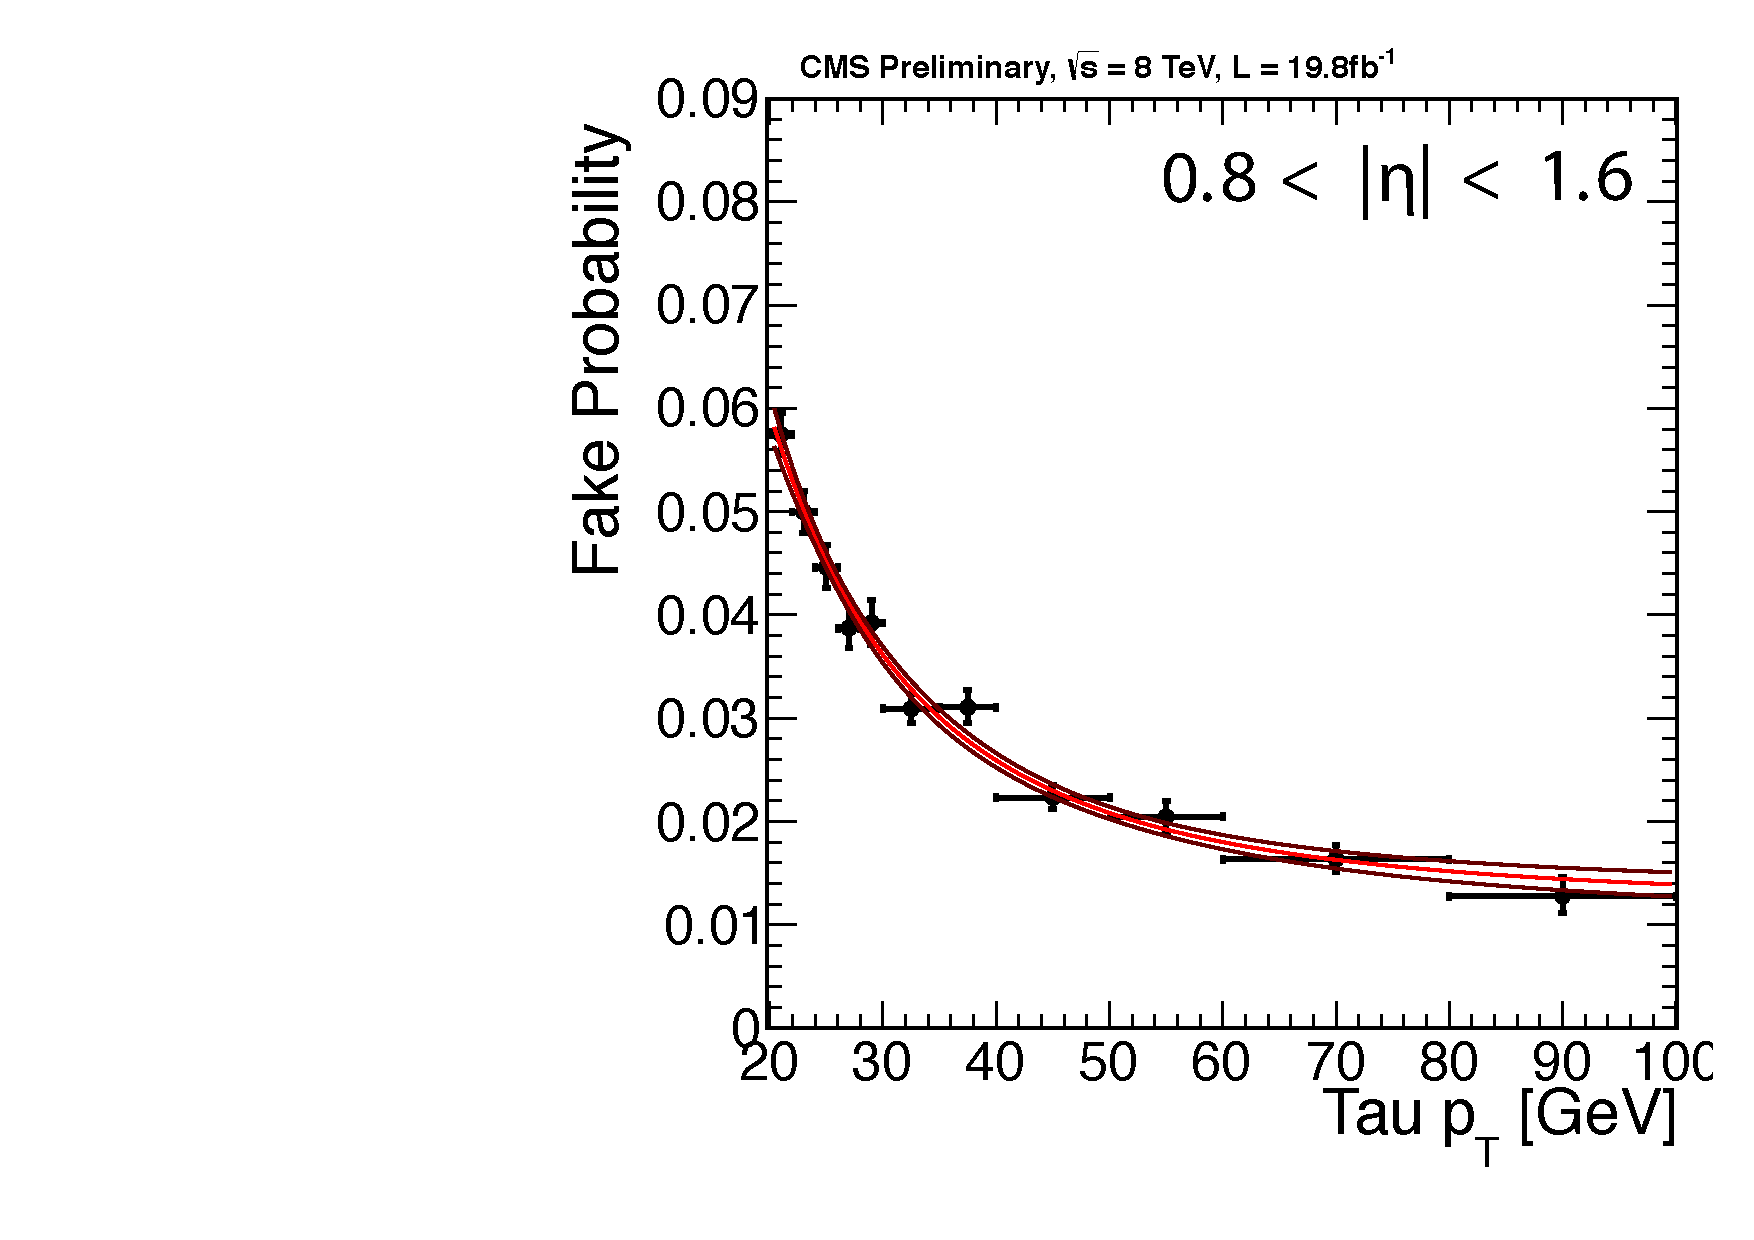
\includegraphics[width=0.33\textwidth]{4_Analisys/pics/8TeV/fakerate_fits/tau_fr_transition.pdf}
  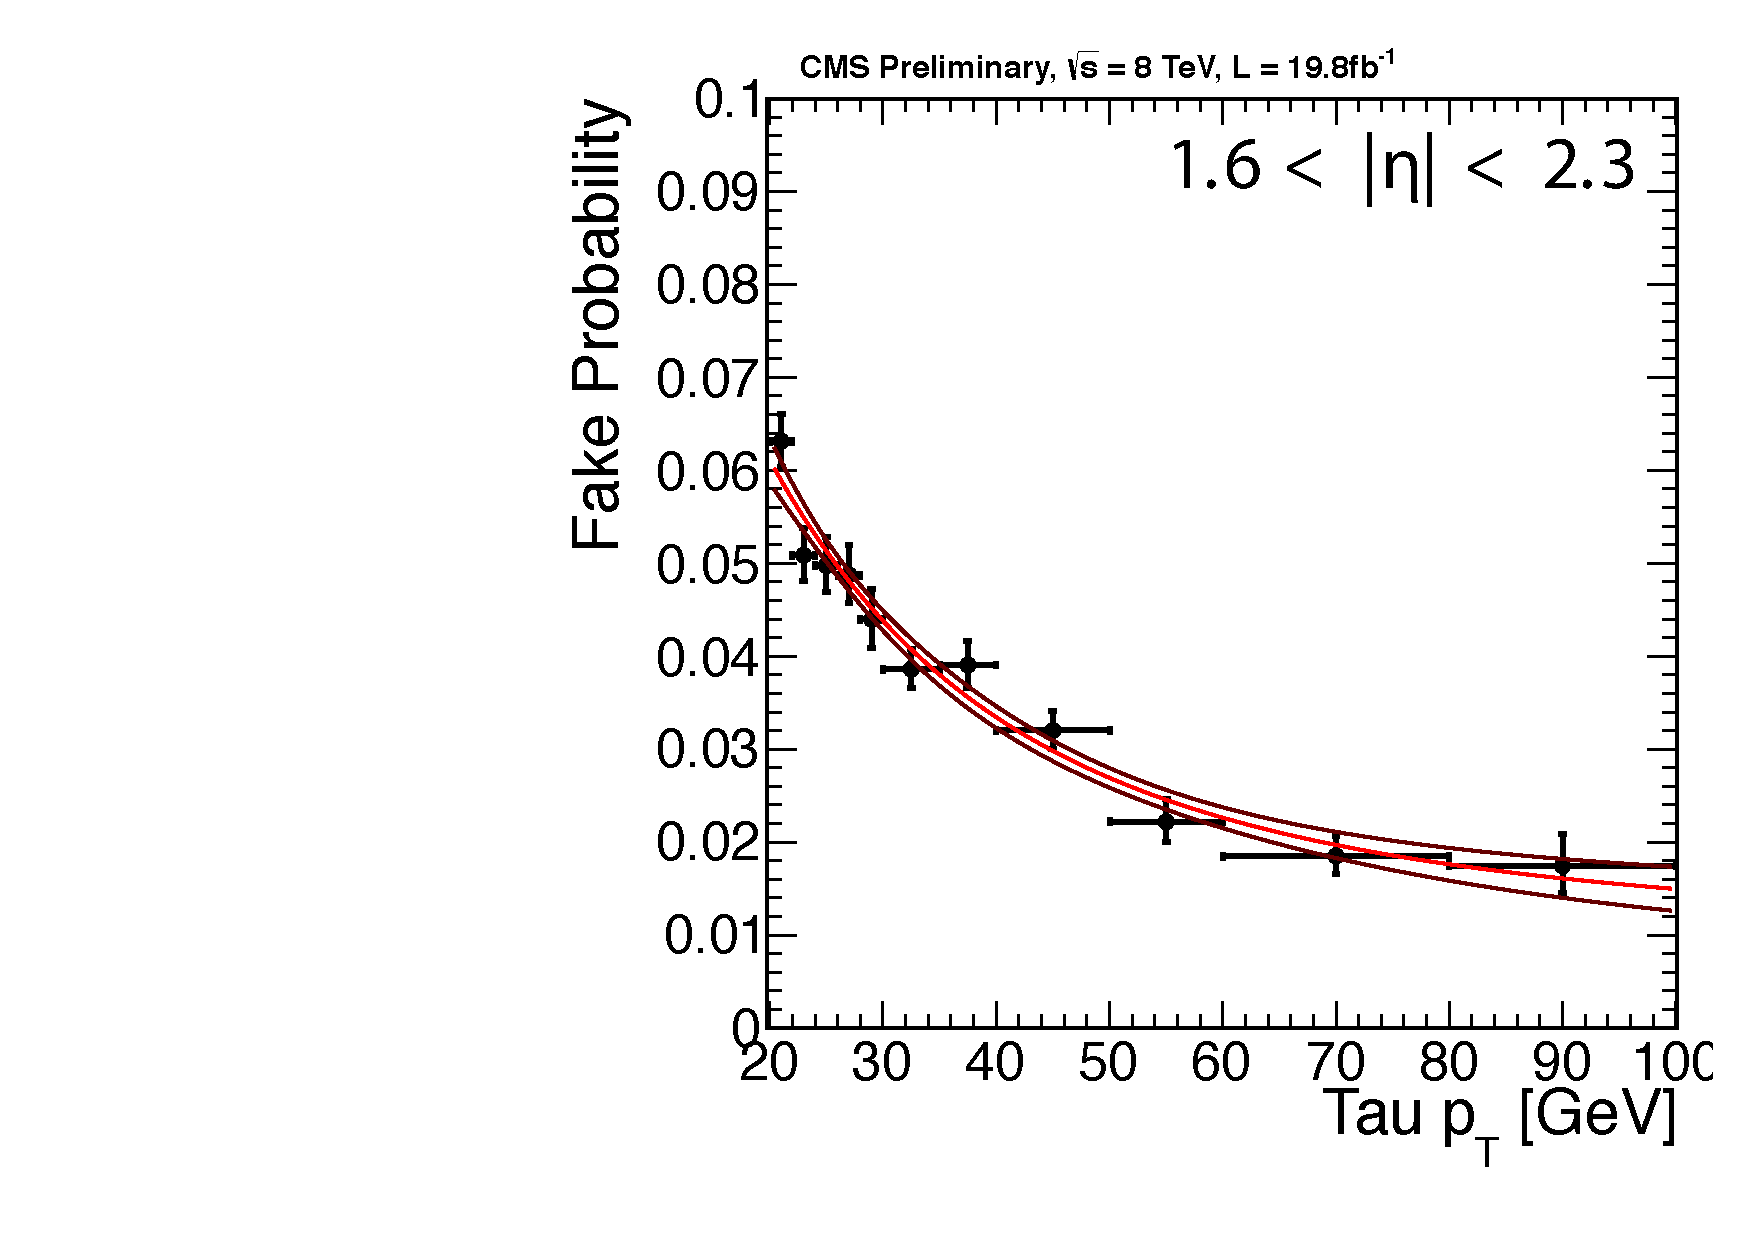
\includegraphics[width=0.33\textwidth]{4_Analisys/pics/8TeV/fakerate_fits/tau_fr_endcap.pdf}
  \caption{Jet $\to \tau_h$ misidentification probability in 7 TeV (top) and 8 TeV (bottom) data, in W$\to \mu$+jet events, as function of tau \pT in barrel (left), transition (center) and endcap (right) regions. The red line shows the result fit to the data.}
  \label{fig:LLT_tau_FR}
\end{figure}


\subsubsection{Background shape extraction}

The tau fake-rate is used to determine a second and completely independent estimate of the reducible background in the signal region.
In this method the tau is considered the possibly mis-identified object and events passing all the analysis selection criteria plus the loose tau
selection but \emph{not} the tight one are weighted according to the measured tau fake-rate to estimate the reducible background.

This method only takes into account those processes in which jets are misidentified as taus. The method cannot account for the Drell-Yan, WW and $t\anti{t}$ reducible backgrounds
in which the reconstructed $\tau_h$ corresponds to a genuine hadronic tau or to an isolated light lepton faking a tau. To account for these types of background the method described in Section \ref{sec:fakemethod}
is applied to simulated events. This procedure is considered to be more reliable than taking the MC expectation in the signal region directly.

The fake tau method was found to produce results consistent with the fake-rate method applied to leptons. To account for possible residual differences,
the fake lepton method was used as nominal value for the reducible background and the estimate obtained from the fake-tau method is used as systematic uncertainty on the background shape.

\subsection{Electron charge mis-identification}
\label{sec:charge_misid}

The most common reason for the mis-measurement of the electron electric charge inside the CMS detector is the interaction of such particle with material in the tracking detectors. % of an  is incorrectly assigned mostly due to a radiative process. 
An electron can radiate a photon, carrying most of its momentum, which may subsequently convert into an $e^+e^-$ pair with highly unbalanced momenta, producing an electron with charge opposite to the initial one that carries most of the initial energy. %If these two processes happen 
In case the bremsstrahlung and the photon conversion processes occur 
in proximity to the interaction point the reconstruction algorithm cannot identify the electron as originating from a conversion.
The description of this process in the simulation is handled by \textsc{GEANT}~\cite{geant}. The probability for an electron to be reconstructed with opposite charge is measured as a function of the electron $\eta$ and \pT using a $\Z \rightarrow ee$ MC sample. The results are shown in figure~\ref{fig:charge_flip_prob_map}.

Another effect associated to the charge mis-measurement is a partial energy loss by radiation that fails to get associated to the electron candidate by the reconstruction algorithm.
This effect causes a shift of the dielectron invariant mass spectrum.
The precision with which this phenomenon is modeled in the simulation is not totally satisfactory. To quantify the effect the spectra of opposite sign (OS) and same sign (SS) electron pairs were fitted with a Cruijfian function (a two-sided gaussian with exponential tails) allowing only a global shifting factor to float. The results of these fits is shown in figure~\ref{fig:ee_invMass_fit}. The process is repeated for both data and simulated events. The value extracted from the former is taken as central value, while the one taken from the latter is used as systematic uncertainty.

The probability for the electron charge mis-measurement is applied as a weight on opposite sign $e^\pm e^\mp \tau_h$ events, which pass the same selection as the signal region, in order to obtain a data-driven estimate for this type of background. The invariant mass distribution obtained with this method is artificially shifted towards lower values 
by the amount computed in the $\Z \rightarrow ee$ data.

\subsection{Control regions}

The background induced by charge misassignment is validated in a dedicated $\Z \To e^\pm e^\pm$ control region.
This region has the same selection as the $ee\tau_h$ signal region with the exception that events containing a tau are removed.
The di-electron invariant mass spectrum in this region is shown in figure~\ref{fig:control_Zee}. The red histogram represents opposite-sign dielectron events weighted by the charge misassignment probability and with the invariant mass scaled by an offset extracted from MC simulation.

\begin{figure}
  \begin{center}
  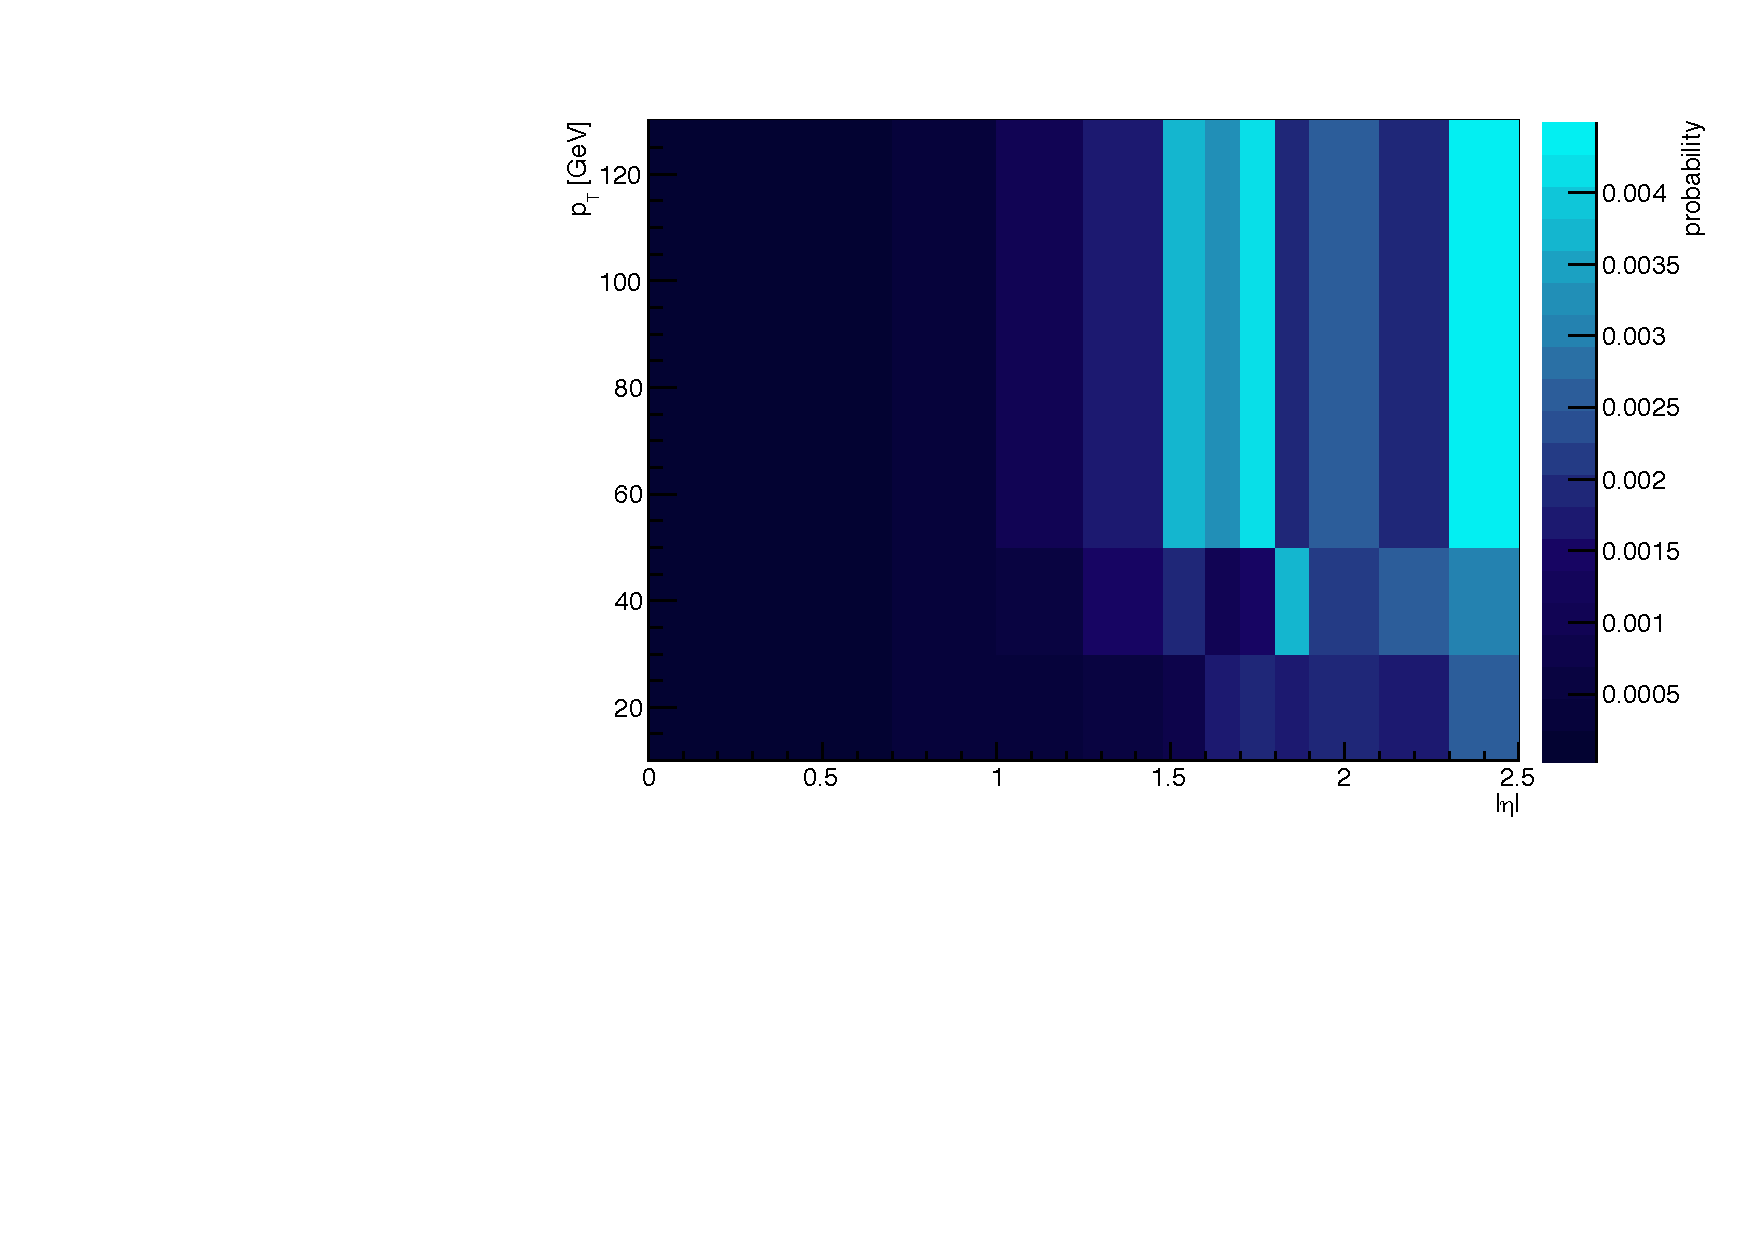
\includegraphics[width=0.8\textwidth]{4_Analisys/pics/8TeV/fakerate_fits/charge_flip_prob_map_eid12Medium_h2taucuts.pdf}
  \caption{
  Electron charge misassignment probability (color scale) as a function of $|\eta|$ and \pT.}
  \label{fig:charge_flip_prob_map}
  \end{center}
\end{figure}


\begin{figure}
  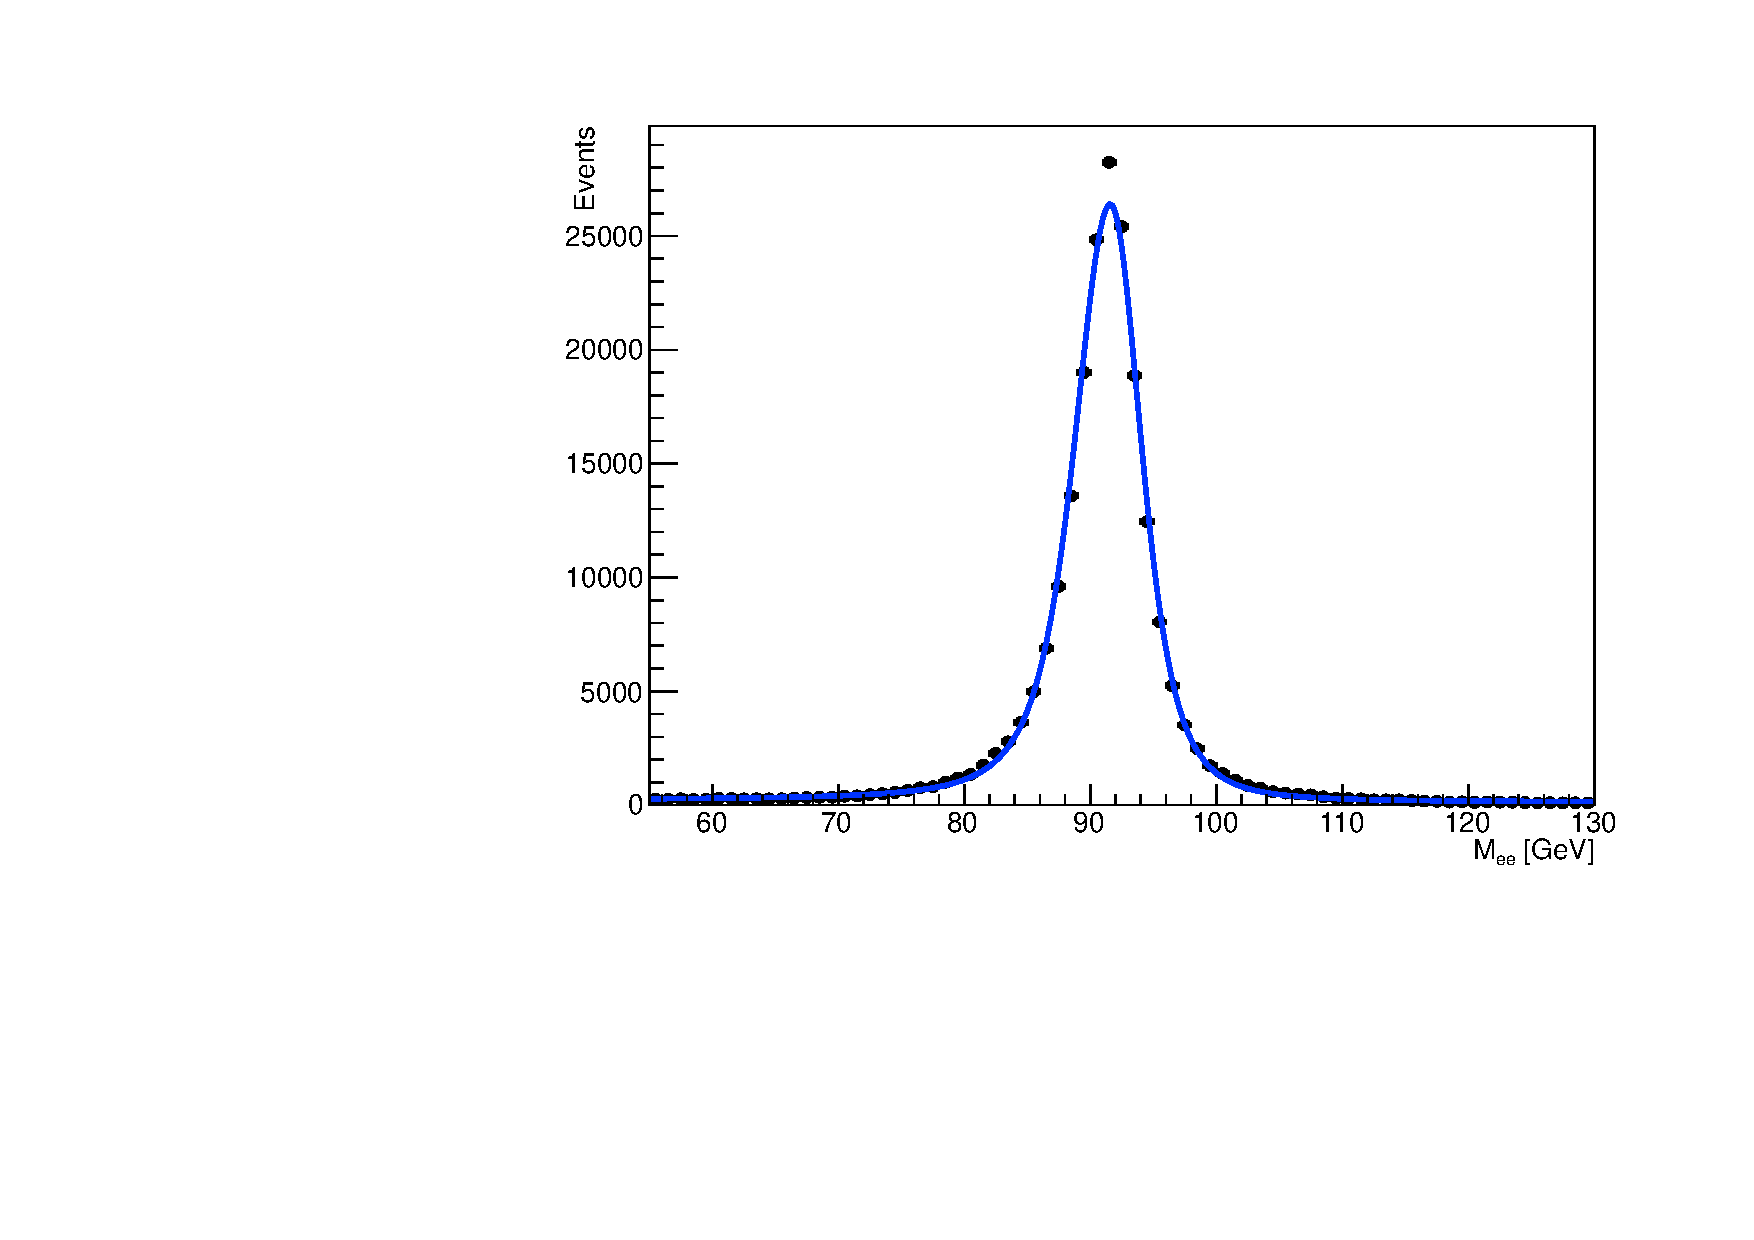
\includegraphics[width=0.5\textwidth]{4_Analisys/pics/8TeV/fakerate_fits/charge_flip_prob_map_eid12Medium_h2taucutsos_trkMass.pdf}
  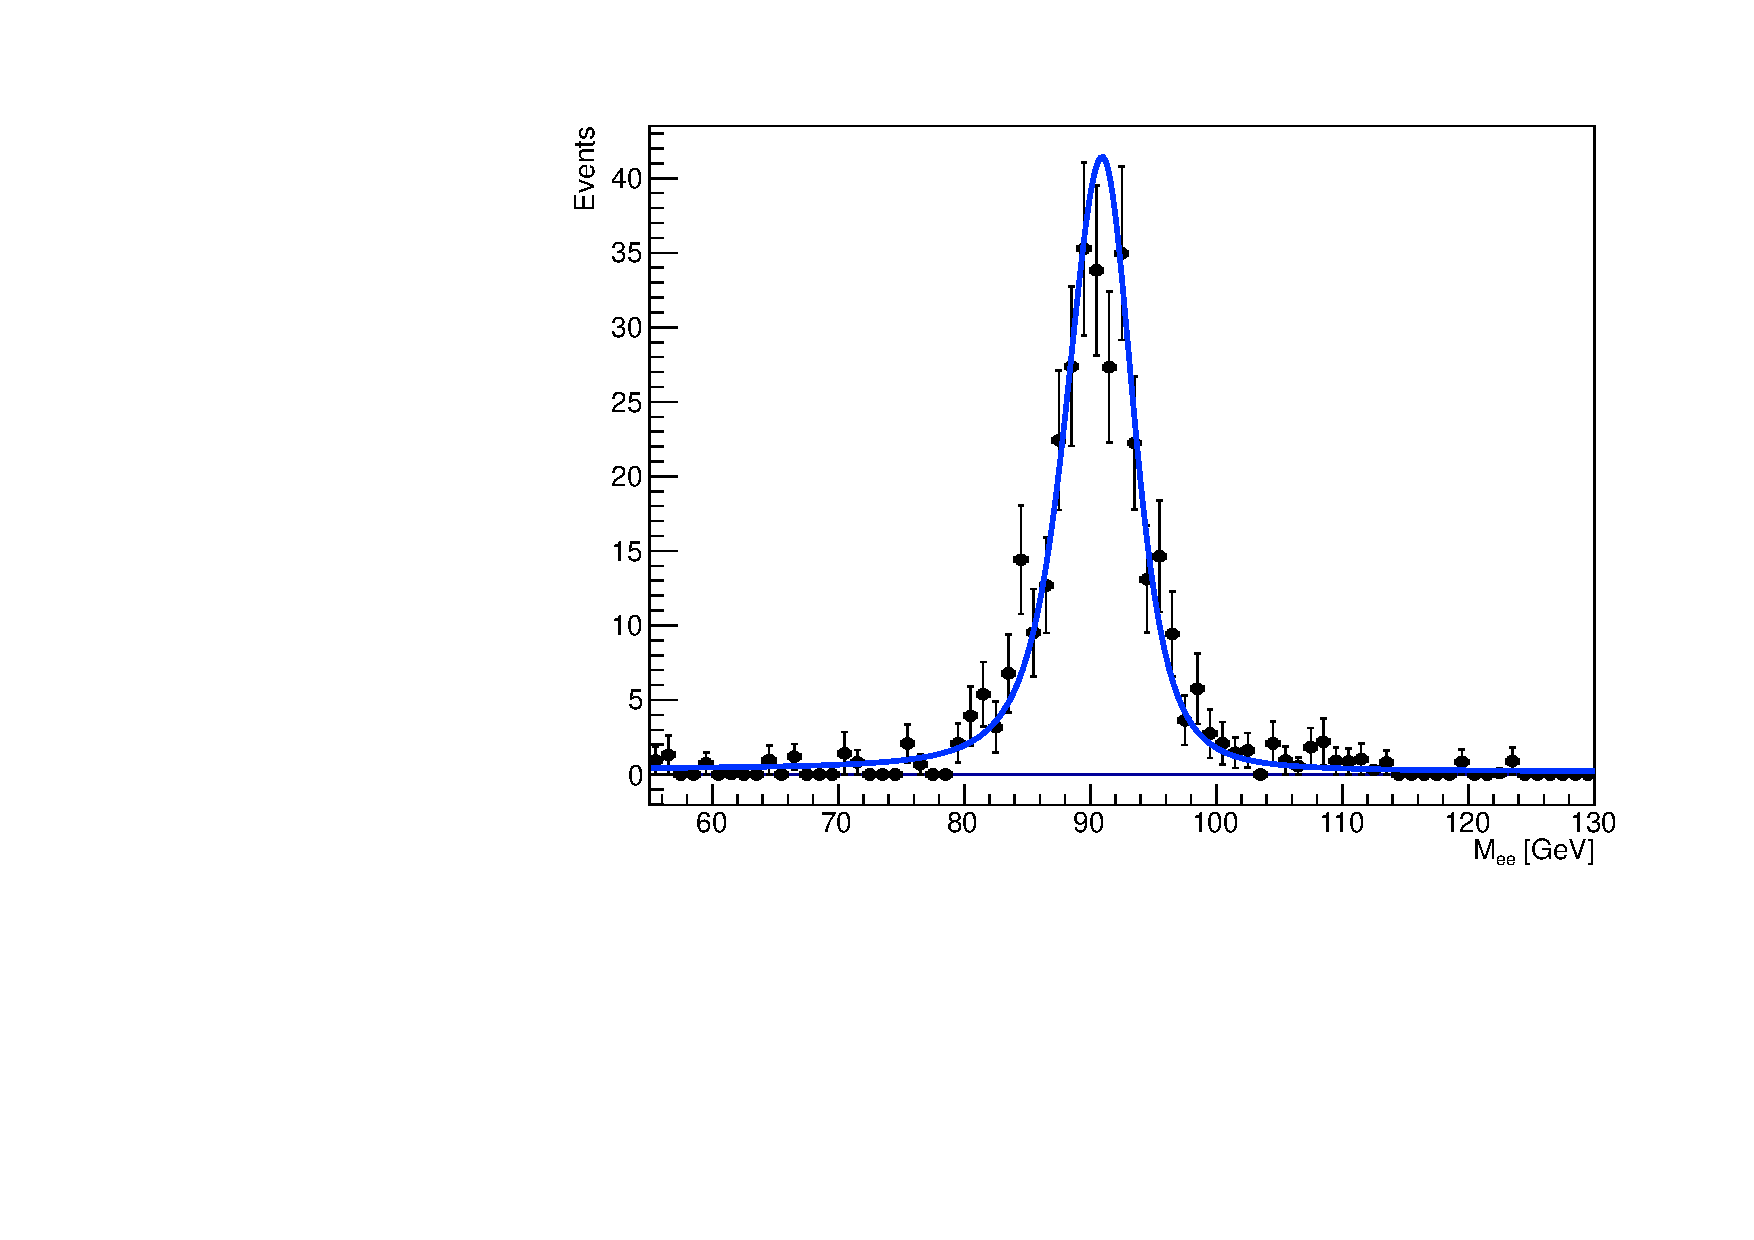
\includegraphics[width=0.5\textwidth]{4_Analisys/pics/8TeV//fakerate_fits/charge_flip_prob_map_eid12Medium_h2taucutsss_trkMass.pdf} \\
  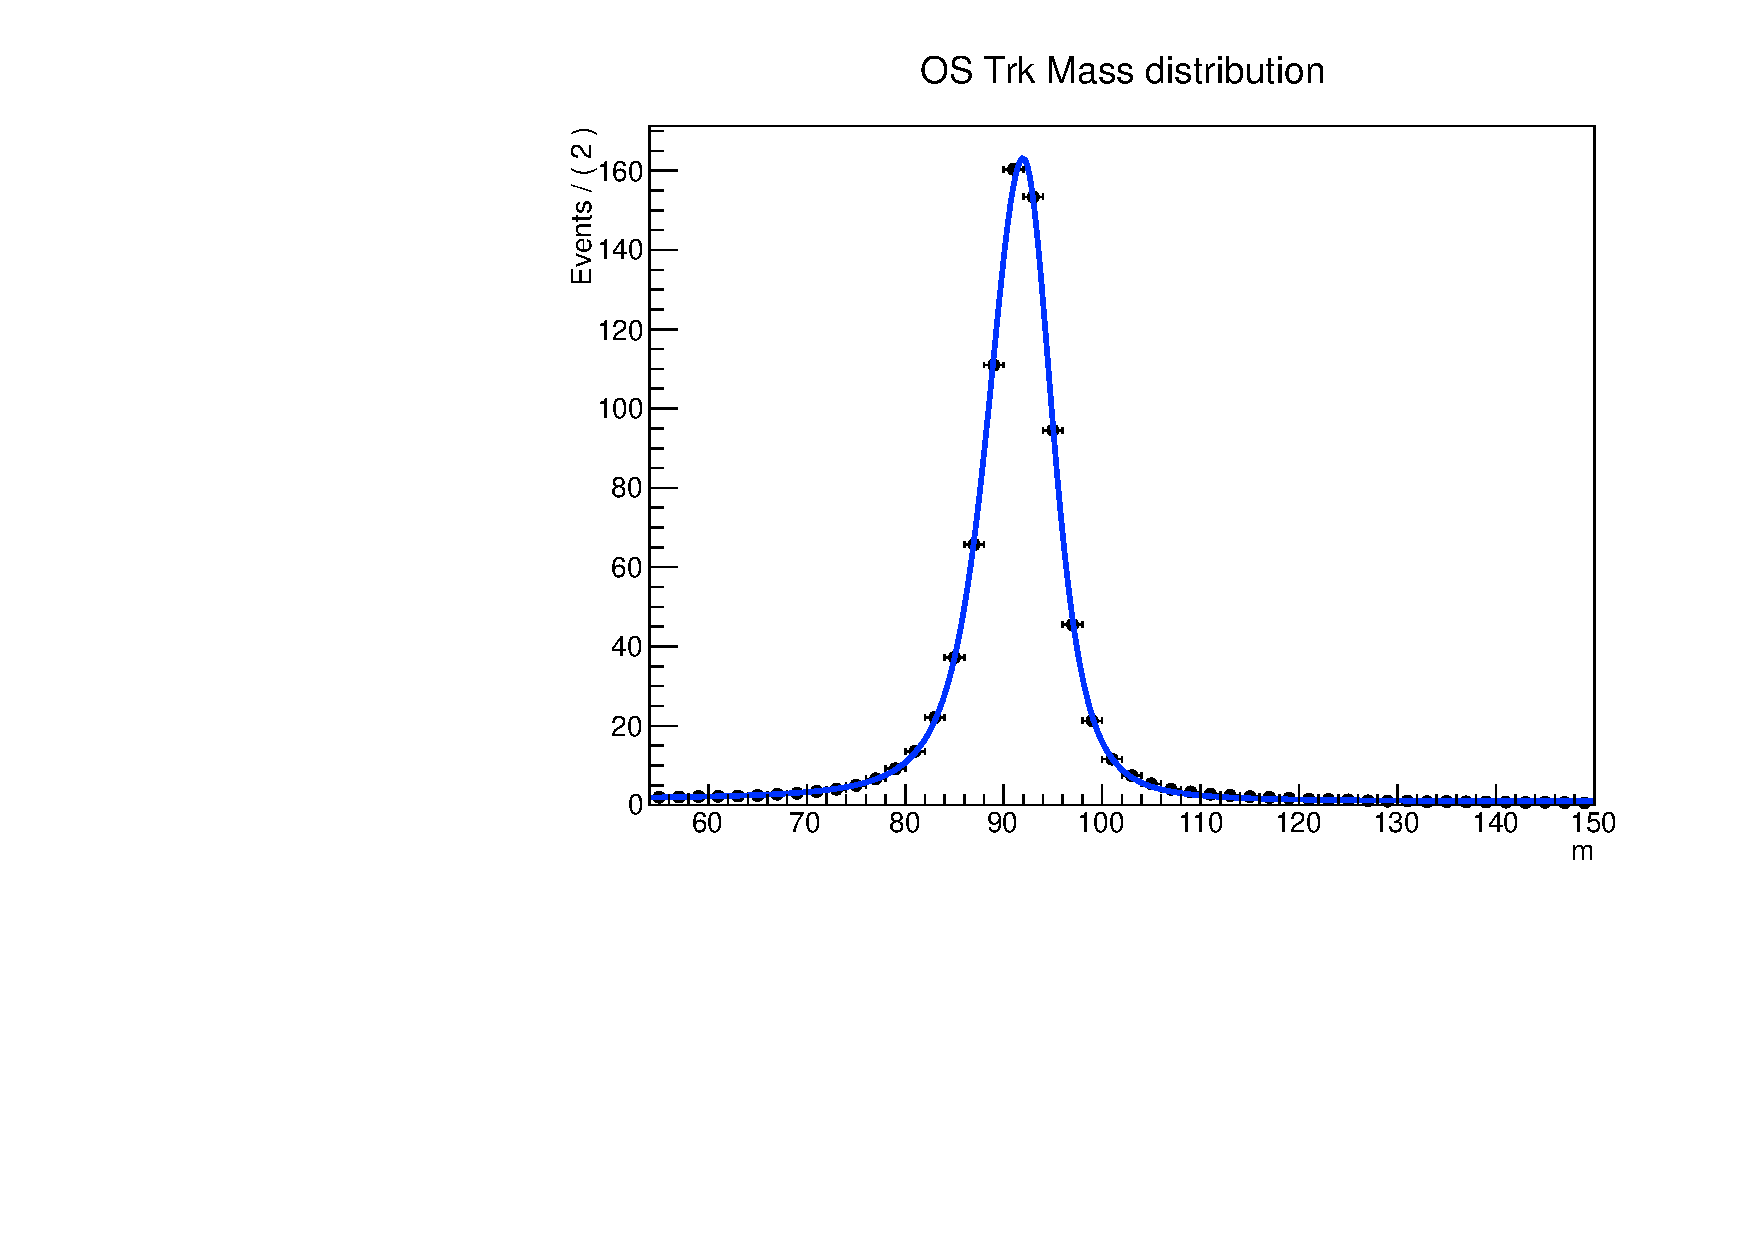
\includegraphics[width=0.5\textwidth]{4_Analisys/pics/8TeV/fakerate_fits/charge_flip_prob_map_dataos_trkMass.pdf}
  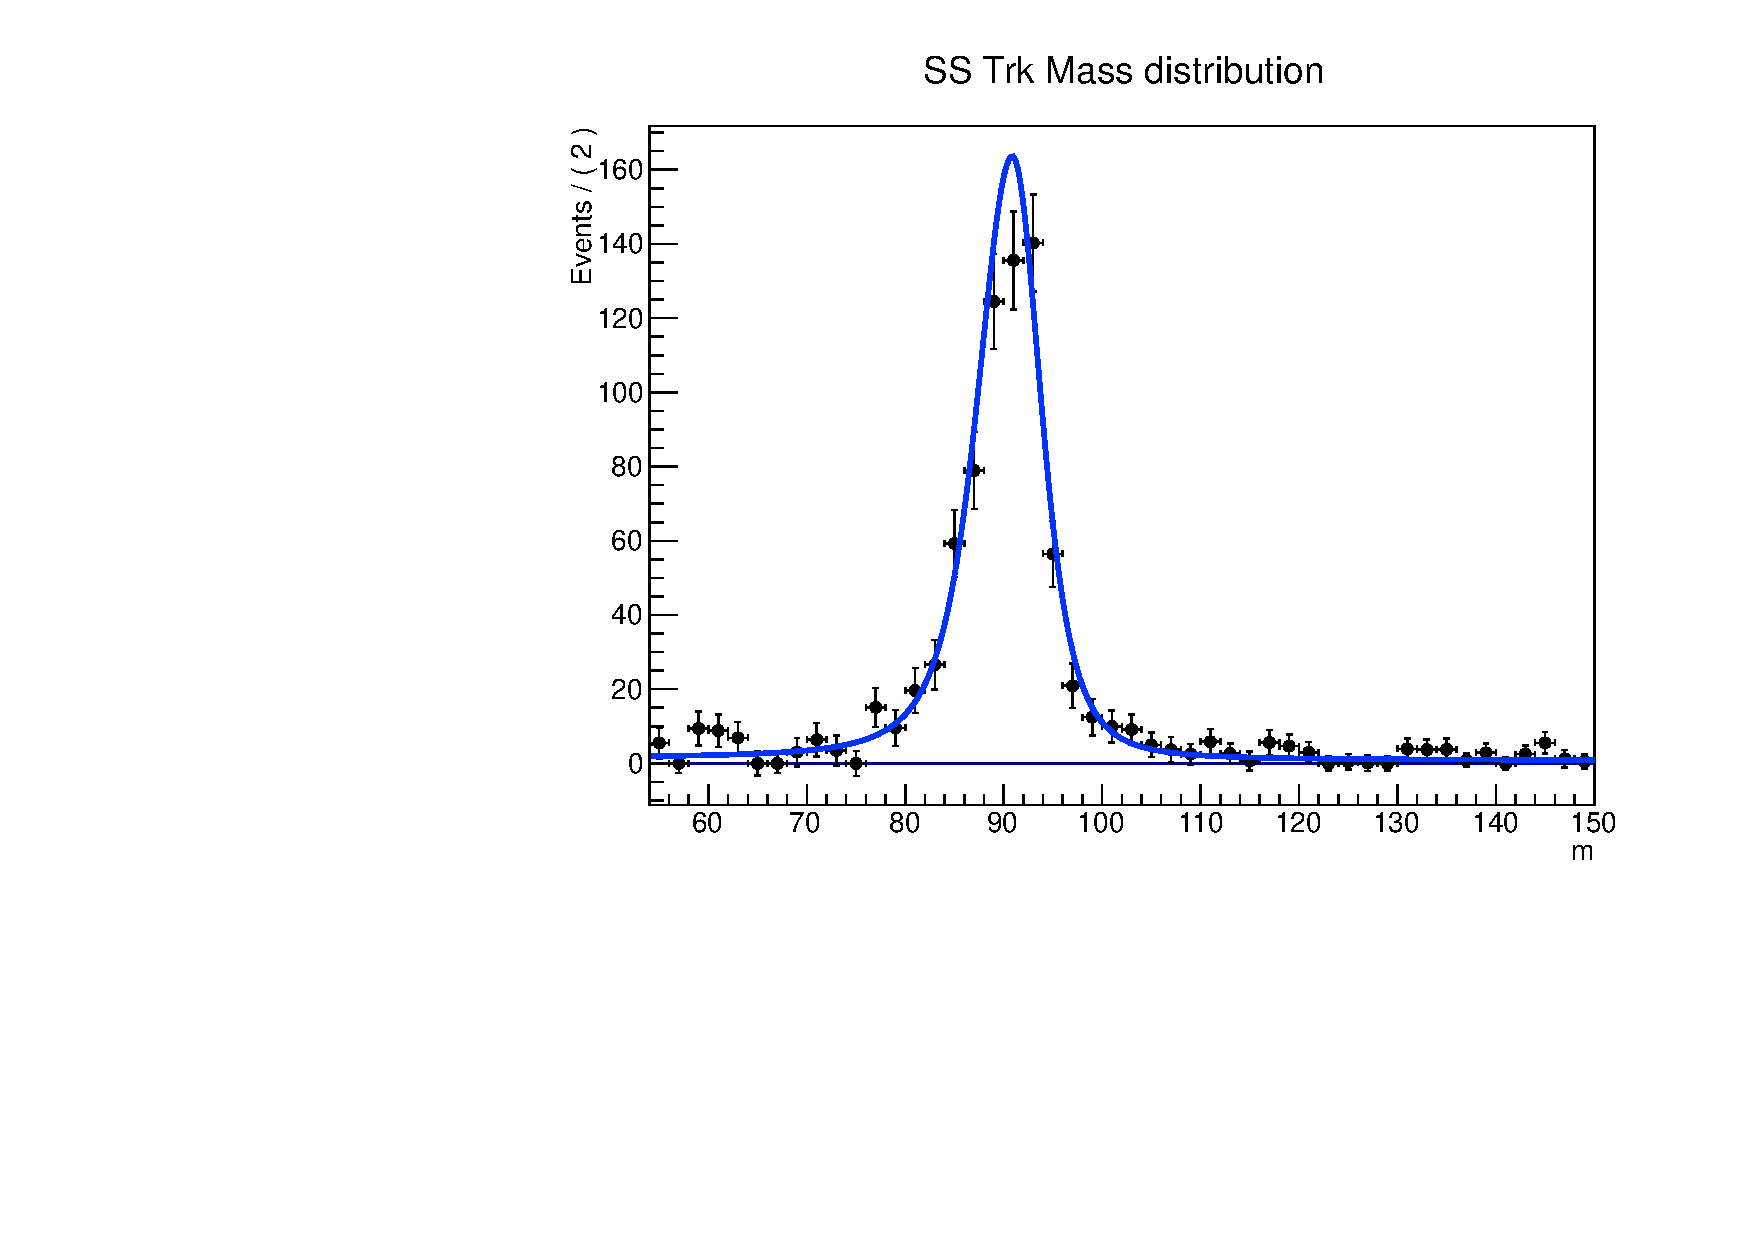
\includegraphics[width=0.5\textwidth]{4_Analisys/pics/8TeV//fakerate_fits/charge_flip_prob_map_datass_trkMass.pdf} \\  
  \caption{
  Comparison of the fit to dielectron invariant mass distributions for opposite-sign (left) and same-sign (right) dielectron candidates from Drell--Yan MC simulation (top) and $\Z\To ee$ data (bottom). The measured invariant mass scale factor is 0.7\% for simulated events and 1.2\% for data}
  \label{fig:ee_invMass_fit}
\end{figure}

\begin{figure}
  \begin{center}
  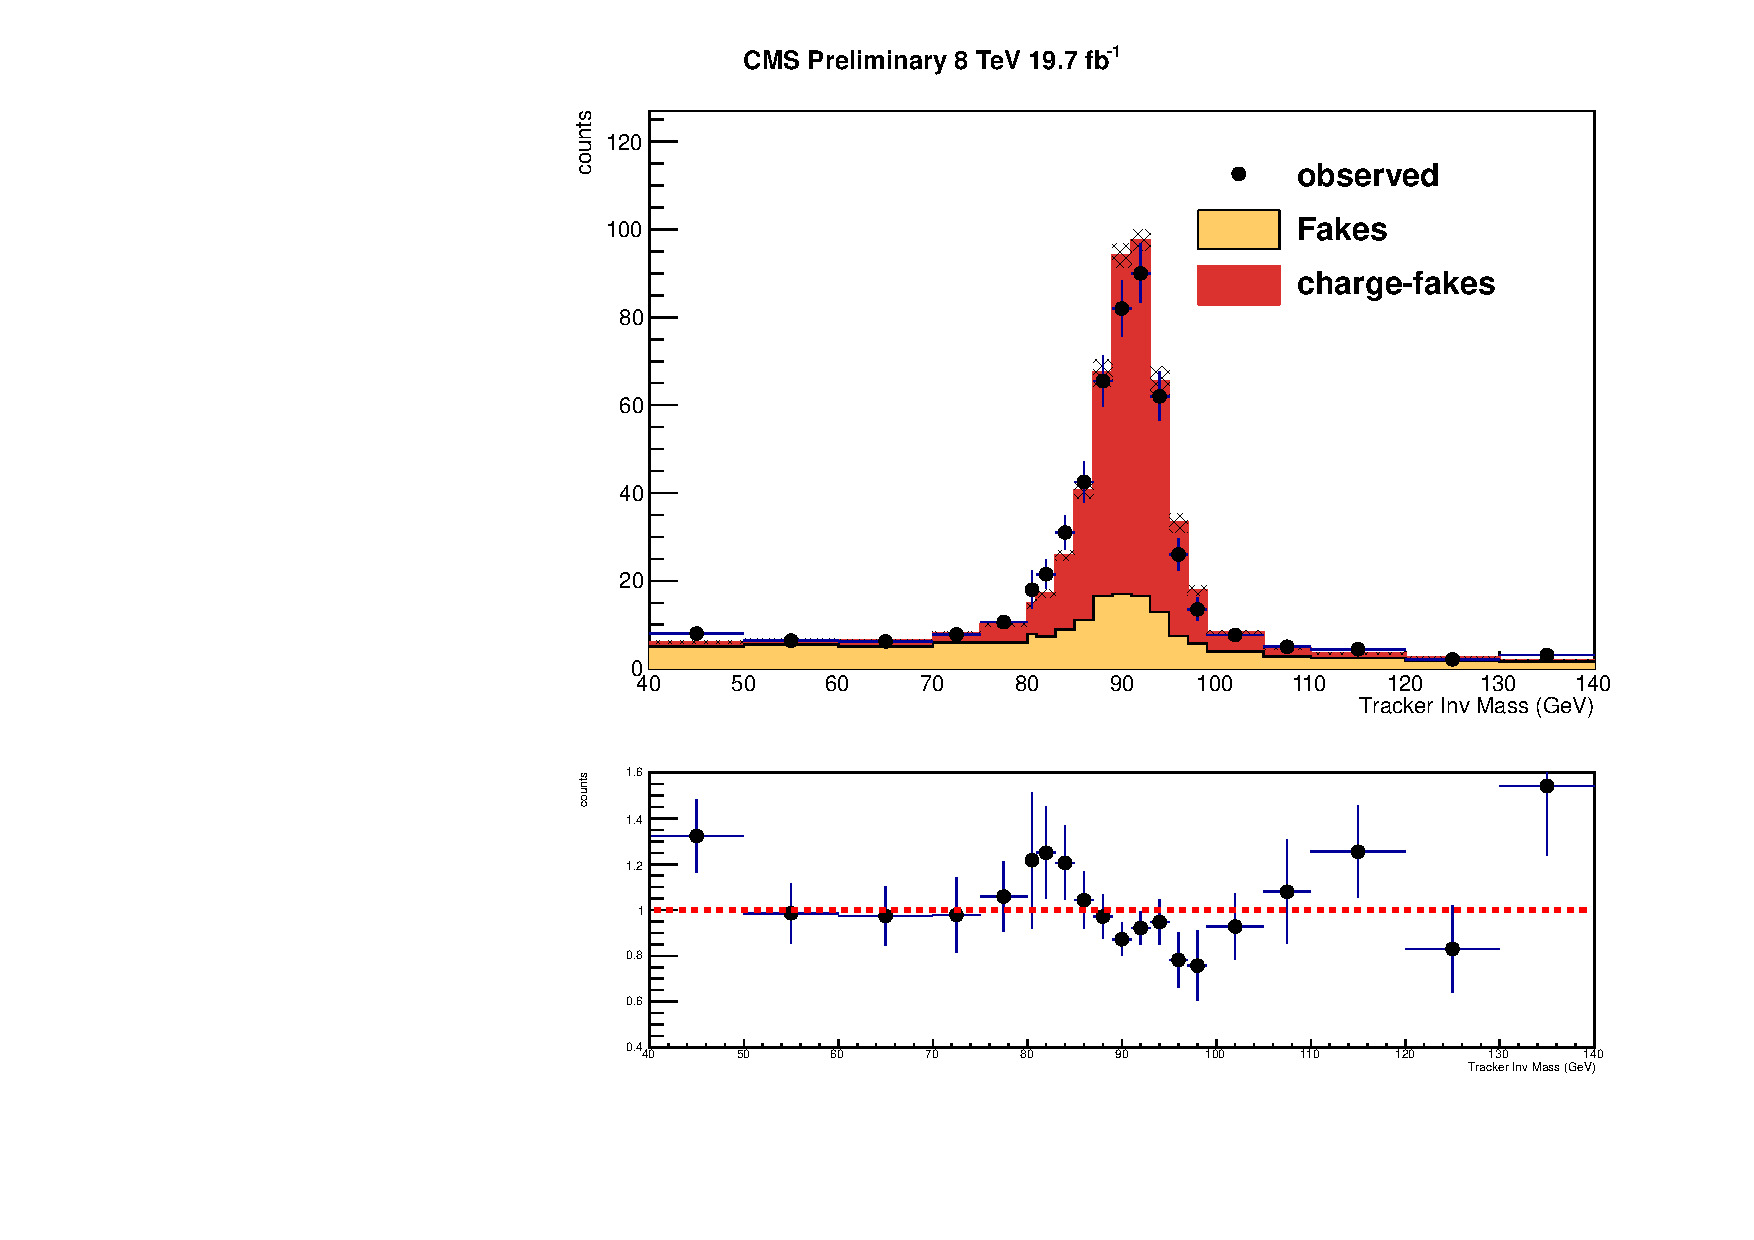
\includegraphics[width=0.8\textwidth]{4_Analisys/pics/8TeV/plots/zee/EE_Charge_Flip_xcheck_trk_invMass.pdf}
  \caption{Invariant mass distribution of same-sign dielectron events: the red histogram is obtained using the information extracted from simulation
(charge misassignment probability and invariant mass scale correction) and applied them to opposite--sign data. The yellow histogram is obtained by applying the fake lepton method to estimate the reducible background.}
  \label{fig:control_Zee}
  \end{center}
\end{figure}

\section{Systematics uncertainties and category optimization}
\label{sec:systematics}

The optimization of the analysis sensitivity and the description of the systematic uncertainties are two subjects that are tightly bound. The figure of merit for %to maximize in 
the optimization is the expected signal significance, while considering the full set of uncertainties correlated for both signal and backgrounds. An optimization purely based on the ``statistical'' significance, defined as $S = N_{sig} / \sqrt{N_{sig} + N_{bkg}}$ may yield an optimal configuration for which the systematic uncertainties are very large.

In this section the definitions and values necessary to have a complete picture of the category optimization process are briefly introduced. The systematic uncertainties are described after the optimization process.
%Once this process will have been fully detailed a more complete description of the systematic uncertainties and their values will be presented. 
A detailed description of how systematic uncertainties are treated to obtain the final result is left for the sections describing the statistical interpretation of the data.

\subsection{Category optimization}

Given the strong dependence of the mis--identification rate on the \pT of the object considered, in particular the hadronic tau, it is quite straightforward to try to improve the signal purity by increasing the threshold on the objects \pT. A better but correlated solution is to use as discriminating observable the scalar sum of the \pT of the three final state leptons, called $L_T$.  

Two types of systematic uncertainties in the background templates are considered in this analysis: normalization uncertainties, which affect only the overall yield of a background, and shape uncertainties, which also affect distribution of the background between bins.

Normalization uncertainties are assigned to account for uncertainties in the luminosity measurement, the correction factors for the trigger emulation, in the identification and isolation efficiencies and in the theoretical cross-sections for all the simulated processes. Normalization uncertainties are also assigned to account for the limited size of the MC samples and the very limited size of the loose-but-not-tight samples that are used to estimate the reducible backgrounds. The last two sources of background are strongly dependent on the category selection and have to be recomputed for each tested configuration.

The difference between the reducible background shape computed with the fake lepton method and the one evaluated with the fake tau method is accounted for by introducing a shape uncertainty that is allowed to vary both the shape and the normalization of the reducible background. 
The same procedure is applied to the reducible background shapes computed with the optimal number of neighbors and the two inferred boundaries. 
Single bin fluctuations in the reducible background shape due to the limited statistics in the anti--isolated regions are separately accounted for by a separate shape uncertainty for each bin (also called \emph{bin--by--bin uncertainties}). Bin--by--bin uncertainties are not allowed to change the total yield of the background process, as this effect is collectively handled by the appropriate normalization uncertainty. It is evident that also these shape uncertainties are dependent on the category selection.

During the optimization two options were tested: either apply a cut rejecting all the events below a certain \LT\ threshold, or divide the events in two categories (called \LT--high and \LT--low) that get fitted simultaneously, increasing the total sensitivity of the analysis. 
For each \LT \ threshold tested the expected frequentist significance of both options has been computed for a SM Higgs boson of 125 GeV. The \LT\ scan was performed by varying the cut threshold between 60 and 170 GeV in 10 GeV steps. 

The categorization is expected to perform \emph{at least} as well as the equivalent cut option, since the \LT--high category alone has the same statistical power as the corresponding cut case. The categorization choice, however, requires a significant amount of data in both the event categories in order for the optimization to be stable. For this reason the categorization option has not been investigated in case of the 7 TeV data. In the 8 TeV $ee\tau_h$ channel the difference between the two options was found to be negligible and therefore the more simple cut was chosen. Figure \ref{fig:LT_scan} show the results of the threshold scans for three channels in the two run periods, while table \ref{tab:LT_options} shows the \LT\ threshold values that maximize the significance for each channel, the reported selection is used to extract the final result.

\begin{figure}
  \includegraphics[width=0.5\textwidth]{4_Analisys/pics/7TeV/limits/mmt.pdf}
  \includegraphics[width=0.5\textwidth]{4_Analisys/pics/8TeV/limits/mmt.pdf} \\
  \includegraphics[width=0.5\textwidth]{4_Analisys/pics/7TeV/limits/emt.pdf}
  \includegraphics[width=0.5\textwidth]{4_Analisys/pics/8TeV/limits/emt.pdf} \\
  \includegraphics[width=0.5\textwidth]{4_Analisys/pics/7TeV/limits/eet.pdf}
  \includegraphics[width=0.5\textwidth]{4_Analisys/pics/8TeV/limits/eet.pdf} \\
  \caption{Expected significance versus \LT\ threshold value for the $\mu\mu\tau_h$ (top), the $e\mu\tau_h$ (center), and the $ee\tau_h$ (bottom) channels in 7 TeV (left) and 8 TeV (right) datasets for two optimization options. The LT threshold is represented by the black dots, the separation of LT event categories by the red boxes.}
  \label{fig:LT_scan}
\end{figure}

\begin{table}
\begin{center}
\caption{Threshold values and categorization approach used in signal extraction for each channel and dataset.}
\label{tab:LT_options}
\begin{tabular}{c c c c}
\hline
Run period & Channel & Best approach & Threshold (GeV) \\
\hline
\multirow{3}{*}{ 7 TeV } & $\mu\mu\tau_h$ & \LT\ Cut & 80 \\	
& $e\mu\tau_h$ & \LT\ Cut & 90 \\
& $ee\tau_h$    & \LT\ Cut & 90 \\
\hline
\multirow{3}{*}{ 8 TeV } & $\mu\mu\tau_h$ & \LT\ Category & 100 \\	
& $e\mu\tau_h$ & \LT\ Category & 110 \\
& $ee\tau_h$    & \LT\ Cut & 70 \\
\hline
\end{tabular}
\end{center}
\end{table}


\subsection{Systematic uncertainties}

As mentioned previously, the sources of systematic uncertainties accounted for in this work can be divided into two groups: the ones affecting only the total normalization of a process, yielding a normalization uncertainty, and the ones also affecting the distribution of the events, yielding a shape uncertainty.

A 2.2\% (2.6\%) uncertainty~\cite{lumi-uncertainty} in the total integrated luminosity is applied to the 7 TeV (8 TeV) simulated samples, respectively. This uncertainty is correlated throughout all the simulated processes, categories and channels belonging to the same running period.
The theoretical uncertainties on %accounted for 
the diboson cross-sections amount to 4\% due to parton distribution function (PDF) plus 4\% due to the QCD renormalization scale. These uncertainties are correlated between all the diboson processes, regardless of channel, category or running period.

The statistical power of the different simulated samples are accounted for by a normalization uncertainty that varies between 3 and 10\% and is uncorrelated between all the channels and categories.

The theoretical uncertainty on the signal cross section due to missing higher orders %the unknown QCD scale 
and due to parton distribution function amounts to 2.7\%~\cite{LHCHiggsCrossSectionWorkingGroup:2011ti}.

The uncertainties on the $e$ and $\mu$ identification, isolation, and trigger efficiencies correspond to the uncertainties on the data-to-simulation correction factors, which have been measured via the tag-and-probe technique\footnote{In a similar manner to what has been described in Section \ref{sec:tauid_eff}, $\Z \To \ell \ell$ events are selected with a single lepton trigger and the desired isolation and identification working points are applied on both leptons. Additionally the invariant mass of the two leptons is required to be within the Z boson mass window: $60 < m_{\ell\ell} < 120$. The trigger efficiencies are computed by applying the trigger requirement to the probe lepton, which does not fire the trigger, both on data and MC. The discrepancies between the two efficiencies, binned in \pT and $\eta$ of the lepton, are applied as a scale factor on the MC and the uncertainty on such correction are taken as systematic uncertainties. A similar tag--and--probe approach on $\Z \To \ell \ell$ events is taken also to correct for discrepancies in the identification and isolation efficiencies.}.
The uncertainty on the $\tau$ identification efficiency is 6\%~\ref{sec:tauid_eff}.
The effect on the simulated yields due to the uncertainty on the electron and $\tau_h$ energy scale has been evaluated.
The electron energy scale uncertainty (1\% for $|\eta| < 1.5$, 2.5\% elsewhere) does not have a measurable effect on the analysis.
Varying the $\tau_h$ energy scale (within a 3\%~\cite{H_tautau} uncertainty) is found to change the expected yields by $3\%$, but has no sizable effect on the observables shapes. A 3\% normalization uncertainty is therefore included.
The uncertainty in the compatibility between simulated and measured efficiency of a light quark or gluon jet to be misidentified as a b-tagged jet, causing the b-veto to 
fail is propagated to the analysis and found to be covered by a 1\% uncertainty in the yields of the simulated samples.

Uncertainties in the reducible background estimation related to the choice of the number of neighbors, k, of the kNN algorithm and in the statistical power of the training sample are computed as described in section \ref{sec:kNN_uncertainties} and propagated to the signal region as a shape uncertainty, which is also allowed to affect the total normalization of the process. The uncertainty is correlated between categories belonging to the same channel and running period.

Uncertainties due to the limited statistical power of the inverted isolation regions that are used to compute the reducible background shape are accounted for by introducing an additional normalization uncertainty that ranges between 12\% and 52\% plus bin--by--bin shape uncertainties. These uncertainties are uncorrelated between all categories and channels.

Finally, the possible mis-modeling caused by the differences in background processes composition between the kNN training sample and the isolation--inverted region is estimated with the ``fake tau'' method and applied as a shape uncertainty, uncorrelated between the different channels and categories.

A 4\% (7\%) uncertainty for each electron candidate in the final state is assigned to account for systematic uncertainties on the charge mis-measurement background yield in addition to the statistical power of the sample for 8 TeV and 7 TeV data, respectively. A 42\% (89\%) uncertainty is assigned to the invariant mass scaling factor (described in section \ref{sec:charge_misid}) that is applied to the shape templates for the charge mis-measured background in the 8 TeV and 7 TeV data, respectively. The uncertainty is applied as a shape uncertainty with no normalization effect. %Both the uncertainties are uncorrelated between channels and running periods. 

A summary of the sources of systematic uncertainties, their values, and their treatment is given in table \ref{tab:systematics}.

\begin{table}
  \begin{center}
    \caption{Systematic uncertainties affecting the $\ell\ell\tau_h$ categories. Values specific to the 2011 datasets are indicated in paranthesis.}
    \label{tab:systematics}
    \begin{tabular}{c c c c}
      \hline
      Source                  & Value & Type & Correlation\\
      \hline
      Luminosity              & $2.2\% (2.6\%)$ & norm. & correlated between channels \\
      $\sigma_{\rm WZ}$        & $4\% \oplus 4\%$  & norm. & fully correlated\\
      $\sigma_{\rm ZZ}$        & $3.3\% \oplus 2.3\%$   & norm. & fully correlated\\
      %$\sigma_{\rm ttW,WWW}  $                  & $100\%$\\
      $\sigma_{\rm H}$ (PDF)   & $2.7\%$  & norm. & fully correlated \\
      diboson MC statistics & $[3\% - 9\%]$ & norm. & fully uncorrelated \\
      signal MC statistics & $[4\% - 12\%]$ & norm. & fully uncorrelated \\
%      \multirow{2}{*}{diboson MC statistics} & $[5\% - 7\%]$ depending on & \multirow{2}{*}{norm.} & \multirow{2}{*}{fully uncorrelated}\\
%      & sample and category & & \\
%      \multirow{2}{*}{signal MC statistics} & $[5\% - 7\%]$ depending on & \multirow{2}{*}{norm.} & \multirow{2}{*}{fully uncorrelated}\\
%      & sample and category & & \\ 
      Tau energy scale        & $3\%$   & norm. & correlated between categories\\
      Tau ID                  & $6\%$ & norm. & correlated between categories\\
      Muon ID + Iso           & $2\%$ & norm. & fully correlated \\
      Electron ID + Iso       & $2\%$ & norm. & fully correlated  \\
      b-tag Fake Rate         & $1\%$ & norm. & fully correlated  \\
      Trigger efficiency  & $1\%$ & norm. & correlated between periods  \\
      fake background statistics & [12\% - 52\%] & norm. & fully uncorrelated \\
      charge mis-ID statistics & [3\% - 26\%] & norm. & fully uncorrelated \\
      kNN training & -- & shape & uncorrelated between channels \\
      fake background composition & -- & shape & fully uncorrelated \\
      charge flip mass scale & -- & shape & uncorrelated between channels \\
      single bin fluctuations & -- & shape & fully uncorrelated \\
      \hline
    \end{tabular}
  \end{center}
\end{table}

\section{Results}

The checks and optimizations have been performed on control regions completely orthogonal to the signal region, or simply based on the expected distributions of known backgrounds. This procedure, called ``blind analysis'', is aimed at reducing as much as possible any bias originating from the choices done by the analyst. 
Once the analysis is considered final, the distribution of observed events in the signal region of each channel are unveiled. 

The physics observable used to discriminate between the signal and the different sources of background is the invariant mass of the visible products of the hadronic tau decay and the sub-leading lepton, $\rm{M}_{\ell_2 \tau}$. The choice of the sub-leading lepton has been found to be about 70\% correlated to the true Higgs decay product, estimated using simulated data. Other observables to assign the correct light lepton as Higgs decay product such as the transverse mass of the lepton and the MET, the lepton isolation or the $\Delta\phi$ between the lepton and the \MET\ have been investigated, but were found to yield inferior correlation with the true Higgs decay products.

The presence of a considerable missing energy source such as the neutrino produced in the W decay does not allow the exploitation of more refined mass reconstruction algorithms such as SVFit.

A summary of the different observed distributions, compared to the respective expectations is shown in figures \ref{fig:LLT_mmt_prefit}, \ref{fig:LLT_emt_prefit}, \ref{fig:LLT_eet_prefit} for the different channels, categories and run periods. Tables \ref{tab:prefit_yields_table_8TeV} and \ref{tab:prefit_yields_table_7TeV} summarizes the expected and observed yields in each category and run period.

\begin{figure}
\begin{center}
  \includegraphics[width=0.49\textwidth]{4_Analisys/pics/7TeV/plots/mmt/LTCut/final-subMass-LTCut.pdf}\\
  \includegraphics[width=0.49\textwidth]{4_Analisys/pics/8TeV/plots/mmt/LTLow/final-subMass-LTLow.pdf}
  \includegraphics[width=0.49\textwidth]{4_Analisys/pics/8TeV/plots/mmt/LTHigh/final-subMass-LTHigh.pdf}\\
  \caption{
  Comparison of $M_{\mu_2\tau}$ spectra observed in data and the background expectation %Comparison of measured and predicted backgrounds 
  in the $\mu\mu\tau_h$ signal region for 7 TeV data (top) and 8 TeV data (bottom). The 8 TeV data is split according the optimal categorization (LT--low on the left and LT--high on the right).
  }
  \label{fig:LLT_mmt_prefit}
\end{center}
\end{figure}

\begin{figure}
\begin{center}
  \includegraphics[width=0.49\textwidth]{4_Analisys/pics/7TeV/plots/emt/LTCut/final-subMass-LTCut.pdf}\\
  \includegraphics[width=0.49\textwidth]{4_Analisys/pics/8TeV/plots/emt/LTLow/final-subMass-LTLow.pdf}
  \includegraphics[width=0.49\textwidth]{4_Analisys/pics/8TeV/plots/emt/LTHigh/final-subMass-LTHigh.pdf}\\
  \caption{
    Comparison of $M_{\ell_2\tau}$ spectra observed in data and the background expectation %Comparison of measured and predicted backgrounds 
  in the $e\mu\tau_h$ signal region for 7 TeV data (top) and 8 TeV data (bottom). The 8 TeV data is split according the optimal categorization (LT--low on the left and LT--high on the right).
  }
  \label{fig:LLT_emt_prefit}
\end{center}
\end{figure}

\begin{figure}
\begin{center}
  \includegraphics[width=0.49\textwidth]{4_Analisys/pics/7TeV/plots/eet/LTCut_7TeV/final-subMass-LTCut_7TeV.pdf}
  \includegraphics[width=0.49\textwidth]{4_Analisys/pics/8TeV/plots/eet/LTCut_8TeV/final-subMass-LTCut_8TeV.pdf}\\
  \caption{
  Comparison of $M_{e_2\tau}$ spectra observed in data and the background expectation %Comparison of measured and predicted backgrounds 
  in the $ee\tau_h$ signal region for 7 TeV data (left) and 8 TeV data (right).
  }
  \label{fig:LLT_eet_prefit}
\end{center}
\end{figure}


\begin{sidewaystable}
%\begin{table}
\caption{Expected event yields for the different background processes and for a 125 GeV WH, $\rm{H}\To\tau\tau$ signal compared to the number of events observed in the data, split by channel and category, for 8 TeV data. The uncertainty quoted in each background process represents statistical plus systematic uncertainty.
%considered in the analysis and number of observed events, divided by channel and category for 8 TeV data. The uncertainty quoted for each background process also includes normalization systematics
}
\begin{center}
\begin{tabular}{c c c c c c c c c}
\hline
\multirow{3}{*}{Process} & \multicolumn{5}{c}{Channels and event categories} \\
& \multicolumn{2}{c}{$\mu\mu\tau_h$} & \multicolumn{2}{c}{$e\mu\tau_h$} & \multirow{2}{*}{$ee\tau_h$} \\
& \LT Low & \LT High & \LT Low & \LT High & \\
\hline
WZ & $ 4.9 \pm 0.6 $ & $ 9.2 \pm 1.0 $ & $ 8.7 \pm 0.9 $ & $ 10.5 \pm 1.1 $ & $ 5.5 \pm 0.6 $ \\
ZZ & $ 0.44 \pm 0.04 $ & $ 0.57 \pm 0.06 $ & $ 0.71 \pm 0.07 $ & $ 0.72 \pm 0.07 $ & $ 0.43 \pm 0.04 $ \\
Reducible Bkg. & $ 9.0 \pm 1.4 $ & $ 6.5 \pm 1.2 $ & $ 9.4 \pm 1.4 $ & $ 8.1 \pm 1.3 $ & $ 7.8 \pm 0.9 $ \\
Charge mis-id. & -- & -- & $ 0.10 \pm 0.01 $ & $ 0.16 \pm 0.02 $ & $ 1.6 \pm 0.1 $ \\
WH, $\rm{H}\To\W\W$ & $ 0.047 \pm 0.004 $ & $ 0.109 \pm 0.009 $ & $ 0.073 \pm 0.006 $ & $ 0.16 \pm 0.01 $ & $ 0.072 \pm 0.006 $ \\
\hline
Total bkg. & $ 14.6 \pm 1.6 $ & $ 17.5 \pm 1.6 $ & $ 19.4 \pm 1.7 $ & $ 21.1 \pm 1.8 $ & $ 16.0 \pm 1.2 $ \\
\hline
WH, $\rm{H}\To\tau\tau$ ($m_\rm{H}=125$ GeV) & $ 0.25 \pm 0.04 $ & $ 1.2 \pm 0.1 $ & $ 0.56 \pm 0.06 $ & $ 1.4 \pm 0.1 $ & $ 0.62 \pm 0.07 $ \\
\hline
Observed & 14 & 12 & 24 & 17 & 13 \\
\hline
\end{tabular}
\end{center}

\label{tab:prefit_yields_table_8TeV}
\end{sidewaystable}
%\end{table}

%\begin{sidewaystable}
\begin{table}
\caption{%Expected yields for the different signal and background processes considered in the analysis and number of observed events, divided by channel and category for 7 TeV data. The uncertainty quoted for each background process also includes normalization systematics
Expected event yields for the different background processes and for a 125 GeV WH, $\rm{H}\To\tau\tau$ signal compared to the number of events observed in the data, split by channel and category, for 7 TeV data. The uncertainty quoted in each background process represents statistical plus systematic uncertainty.}
\begin{center}
\begin{tabular}{c c c c c c c c c}
\hline
\multirow{2}{*}{Process} & \multicolumn{3}{c}{Channels} \\
& $\mu\mu\tau_h$ & $e\mu\tau_h$ & $ee\tau_h$ \\
\hline
WZ & $ 2.3 \pm 0.3 $ & $ 3.6 \pm 0.4 $ & $ 1.2 \pm 0.1 $ \\
ZZ & $ 0.43 \pm 0.04 $ & $ 0.64 \pm 0.07 $ & $ 0.24 \pm 0.02 $ \\
Reducible Bkg. & $ 0.4 \pm 0.2 $ & $ 1.2 \pm 0.5 $ & $ 1.2 \pm 0.3 $ \\
Charge mis-id. & -- & $ 0.04 \pm 0.01 $ & $ 0.38 \pm 0.06 $ \\
WH, $\rm{H}\To\W\W$ & $ 0.035 \pm 0.003 $ & $ 0.055 \pm 0.005 $ & $ 0.020 \pm 0.002 $ \\
\hline
Total bkg. & $ 3.5 \pm 0.4 $ & $ 6.0 \pm 0.7 $ & $ 3.3 \pm 0.3 $ \\
\hline
WH, $\rm{H}\To\tau\tau$ ($m_\rm{H}=125$ GeV) & $ 0.33 \pm 0.03 $ & $ 0.45 \pm 0.05 $ & $ 0.18 \pm 0.02 $ \\
\hline
Observed & 3 & 4 & 5 \\
\hline
\end{tabular}
\end{center}

\label{tab:prefit_yields_table_7TeV}
%\end{sidewaystable}
\end{table}


\section{Limit setting procedure and results}

\subsection{Statistical framework}
The binned $\rm{M}_{\ell_2 \tau}$ distributions of each channel and category have been used for the statistical interpretation of the results. The choice of the binning, reflected in the plots shown in the previous section, represents a compromise between granularity and event population of each bin. The final choice for 8 TeV data is 10 GeV wide bins between 20 and 80 GeV followed by a 20 GeV wide bin up to 100 GeV and a 30 GeV wide bin up to 130 GeV; finally a 70 GeV wide bin covers the invariant mass region between $130 < M_{\ell 2 \tau} < 200$ GeV. In the 7 TeV data, the small dataset size forces a much wider binning, leading to the choice of a 20 GeV wide bin between 20 and 40 GeV, followed by 40 GeV wide bins up to 120 GeV plus a single bin extending up to 200 GeV.



{\color{red}
The expected background and signal distributions are fitted to the data to infer the value of the signal normalization, $\mu$, by maximizing a likelihood function.
The likelihood function is formulated in terms of $\mu \cdot s(\boldtheta) + b(\boldtheta)$, where $b(\boldtheta)$ denotes the expected background yield and distribution, while $s(\boldtheta)$ denotes the expected distribution of the signal process. Both $b(\boldtheta)$ and $s(\boldtheta)$ depend on the ensemble of \emph{nuisance parameters} ($\boldtheta$), which represent the statistical and systematic uncertainties in the background predictions. The multiplicative $\mu$ parameter in front of $s(\boldtheta)$, known as \emph{signal strength modifier}, is the parameter of interest which describe the strength of the observed signal with respect to the expected SM value ($\sigma_{obs}/\sigma_{SM}$). The value of the $\mu$ parameter is allowed to become negative to avoid any bias in the fit.

The likelihood implemented in the fit is defined as the product of the likelihoods for each category times the likelihood function for the nuisance parameters:
}
\begin{equation}
\mathcal{L}(obs|\mu, \boldtheta) = \prod^{cat} \mathcal{L}_c(obs|\mu, \boldtheta) \times \prod^{nuisance} p(\hat{\theta},\theta) = \operatorname{Poisson}(obs_c, \mu, \boldtheta) \times \prod^{nuisance} p(\hat{\theta},\theta),
\end{equation}

where

\begin{equation}
\operatorname{Poisson}(obs_c, \mu, \boldtheta) = \dfrac{(\mu s_i(\boldtheta) + b_i(\boldtheta))^{n_i}}{n_i!}e^{(\mu s_i(\boldtheta) + b_i(\boldtheta))}.
\end{equation}

As described in section \ref{sec:systematics}, two kinds of systematic uncertainties were considered. Systematic uncertainties associated to the overall normalization are considered to be distributed according to a \emph{log--normal} distribution:

\begin{equation}
\rho(\theta, \hat{\theta}) = \dfrac{1}{\theta\sqrt{2\pi}\opname{ln}(k)} e^{-\left(\dfrac{\opname{ln}(\theta/\hat{\theta})}{\sqrt{2}\opname{ln}k}\right)^2}
\end{equation}

with $k = 1+ \epsilon$, where $\epsilon$ is the size of the yield uncertainty.

Shape uncertainties are modeled using three distributions: the distribution for the central value plus the templates for the upward and downward shifts by one standard deviation of the respective nuisance parameter. A family of distributions is obtained starting from these three templates using a morphing technique. The morphing function interpolates the contents of each bin as a function of the nuisance parameter. The interpolation is quadratic within the boundaries provided by the two additional shifted templates and linear beyond this point. A gaussian distribution with mean 0 and $\sigma = 1$ is assigned to the single morphing parameter. The extrapolation is built in such a way that the nuisance parameter assumes the value 0 for the central template and the values $\pm1$ for the shifted templates. More details on this ``vertical morphing'' technique can be found in \cite{Conway:2011in}.

{\color{red}
In case the fit shows no significant presence of signal, which is related to a negative value of $\mu$ or compatible with zero, exclusions limit can be set.
}


The exclusion limit of a SM Higgs boson is statistically performed by evaluating the compatibility of the data to two hypotheses: the \emph{null hypothesis} $H_0$, which corresponds to the absence of a Higgs boson signal, and the  \emph{alternative hypothesis}, which includes the presence of a Higgs signal. The discrimination between the two hypotheses is performed by defining a test statistic under the null hypothesis and compute its value under the observed data case. The observed value of this test statistic, with respect to the theoretically expected distribution, allows to compute the probability to observe a compatibility to $H_0$ worse than the observed one. Such probability is called \emph{p--value} and is used to take the decision whether to reject the hypothesis $H_0$ in favor of $H_1$ or not.

The theoretical framework under which the test statistics is built represents a modified version of the CL$_s$ method \cite{CLs} and follows the prescriptions agreed between the ATLAS and CMS statistical committees for Higgs boson searches \cite{higgscombo}.

{\color{red}
The null hypothesis is formulated in terms of only the expected backgrounds distributions $b(\boldtheta)$ defined previously, while 
the $H_1$ hypothesis is formulated as the sum of signal and backgrounds, $\mu \cdot s(\boldtheta) + b(\boldtheta)$, as initially shown.
}

%The setting of a 95\% confidence limit on the presence of the Higgs boson can therefore be reduced to the computation of the value $\mu_{up}$ which leads to $p(H(\mu_{up}\cdot s + b)) < 0.05$ with observed data.

According to the Neyman-Pearson lemma, the most powerful test statistics to discriminate between the $H_0$ (background only) and the $H_1$ (signal plus background) hypotheses is the \emph{profile likelihood ratio} $\lambda$, defined as:

\begin{equation}
\label{eq:likeratio}
\lambda(\mu) = -2 \operatorname{ln} \dfrac{\mathcal{L}(obs | \mu \cdot s + b, \thetahat_\mu)}{\mathcal{L}(obs | \muhat \cdot s + b, \thetahat)},
\end{equation}

%where $\thetahat$ and $\hat{\mu}$ are the set of nuisance values and the value of $\mu$ that maximize the likelihood (called \emph{maximum likelihood estimator}) and $\thetahat_\mu$ is the maximum likelihood estimator of the nuisances for a fixed value of $\mu$.
where $\thetahat$ represents the set of nuisance parameter values that maximize the likelihood (called \emph{maximum likelihood estimator}) and $\thetahat_\mu$ are the values of the nuisance parameters that maximize the likelihood for a fixed value of $\mu$.

Equation \ref{eq:likeratio} is complemented by the boundary condition $0 \leq \muhat \leq \mu$ that ensures that the expected signal yield is positive and that the computed confidence interval is one sided (and therefore $\mu \geq \muhat$). These conditions are imposed on the test statistic by forcing $\muhat = 0$ even when the fit yields as best result a negative value and by setting the test statistic to 0 when $\mu < \muhat$.

\begin{equation}
q(\mu) = \left\{\begin{matrix}
-2 \operatorname{ln} \dfrac{\mathcal{L}(obs | \mu \cdot s + b, \thetahat_\mu)}{\mathcal{L}(obs | \muhat \cdot s + b, \thetahat)} & , \muhat < 0\\ 
-2 \operatorname{ln} \dfrac{\mathcal{L}(obs | \mu \cdot s + b, \thetahat_\mu)}{\mathcal{L}(obs | \muhat \cdot s + b, \thetahat)} & ,0 \leq \muhat \leq \mu \\ 
0 & , \mu < \muhat
\end{matrix}\right.
\label{eq:test_stat}
\end{equation}

%Under this definition small values of 
The test statistic $q(\mu)$ is defined such that small (large) values indicate preference for the $H_1$ ($H_0$) hypothesis.

%Under the assumption of large samples 
In the limit of large event statistics the distribution of the test statistic $q_\mu$ under both hypotheses collapse into well-defined analytical functions as described by the Wilkins theorem and reported in \cite{Cowan:2010js, higgscombo}. This assumption allows to compute the p-value, i.e. the probability to observe data less compatible with the null hypothesis than the observed one, under a specific hypothesis with a numerical integration rather than toy MC methods.

A naive approach to limit setting would be computing, for each mass point, the value $\mu_{up}$ for which $p(q(\mu_{up}) | H_1) = \int_{q_{\mu,obs}}^{\infty}f(q_\mu|H_{\mu_{up}})dq_\mu = 0.05$. This approach would not be safe in case of background under-fluctuations and a small expected signal. In this case the value $p(q(\mu_{up}) | H_0)$ is also a small number, potentially very close to the threshold of 0.05. This would lead to a paradox in which both $H_1$ \emph{and} $H_0$ have to be rejected.

In this situation data are not sufficient to reject the $H_1$ hypothesis. To overcome this effect the \CLs\ method defines the confidence level as:

\begin{equation}
CL_s(\mu) = \dfrac{CL_{s+b}}{CL_b} = \dfrac{p(q(\mu) | H_1)}{p(q(\mu) | H_0)}
\end{equation}

The immediate consequence of this definition is that small values of $\mu$ become harder to exclude.

\subsection{Fit results}

The reliability of the background modeling and of the systematic uncertainty model can be tested by analyzing the ancillary output of the profile maximum likelihood fit performed during the CL$_s$ limit computation. A common practice is to compute the values:

\begin{equation}
\dfrac{\hat{\theta} - \theta}{\sigma_{\theta}},
\end{equation}

which are the difference between the best--fit (post-fit) value and the central (pre-fit) value of the nuisance parameter, divided by its expected uncertainty. This quantity is commonly referred to as \emph{pull}. The maximum likelihood fit also evaluates the a posteriori variance of each nuisance parameter. Large outliers in the pull distribution can indicate an under-estimation of the systematic uncertainty associated to the corresponding nuisance parameter. Very small a posteriori variance of a nuisance indicates that the data are constraining a certain systematic uncertainty to a better degree than the a priori knowledge. This effect is not necessarily a flaw in the modeling, but requires additional scrutiny to ensure that the correlation of such nuisance parameter among different categories is well motivated. This effect is widely exploited when creating a category with large number of selected events and low sensitivity on the sole purpose of constraining one or more systematic effects on a more sensitive, but small size, category. 

Table \ref{tab:pulls} summarizes the largest pulls observed in the maximum likelihood (ML) fit to the data.

\begin{table}
\caption{List of all the nuisance parameters which pull ($\Delta x/\sigma_{\text{in}}$) is either larger than $\pm0.3$ or the a posteriori variance ($\sigma_{\text{out}}/\sigma_{\text{in}}$) changed by more than 10\% with respect to the a priori one. $\Delta x$ denotes the shift in the nuisance value that best fits the data and $\sigma_{\text{in}}, \,\sigma_{\text{out}}$ represent the a priori and a posteriori variance of the nuisance parameter, respectively.}
\begin{tabular}{c c c c } \hline 
\multirow{2}{*}{ Sample } & \multirow{2}{*}{Channel} & \multirow{2}{*}{name} &     $b$-only fit \\
 &  & &  $\Delta x/\sigma_{\text{in}}$, $\sigma_{\text{out}}/\sigma_{\text{in}}$ \\  
\hline
\multirow{5}{*}{ 7 TeV } & \multirow{3}{*}{ $\mu\mu\tau_h$ } & Reducible bkg. Bin-by-bin bin \#2   &      -0.20, 1.08 \\
& & Reducible bkg. Bin-by-bin bin \#4      &      +0.14, 1.68 \\
& & kNN shape uncertainty           &      -0.04, 0.83 \\
 \cline{2-4}
& $e\mu\tau_h$ & Reducible bkg. Bin-by-bin bin \#1      &      +0.20, 0.85 \\
 \cline{2-4}
& $ee\tau_h$ & Reducible bkg. Bin-by-bin bin \#3      &      -0.31, 1.03 \\
 \hline
\multirow{11}{*}{ 8 TeV } & \multirow{3}{*}{ $\mu\mu\tau_h$ } & Reducible bkg. normalization, $L_T$ high   &      -0.30, 0.95 \\
& & Reducible bkg. composition, $L_T$ high    &      -0.35, 0.67  \\
& & Reducible bkg. Bin-by-bin bin \#1 &      +0.25, 0.88 \\
& & Reducible bkg. Bin-by-bin bin \#7 &      -0.35, 1.00 \\
& & Reducible bkg. composition, $L_T$ low     &      +0.32, 0.64  \\
& & kNN shape uncertainty          &      +0.25, 0.82  \\
 \cline{2-4}
& \multirow{4}{*}{ $\mu\mu\tau_h$ } & Reducible bkg. composition, $L_T$ high    &      +0.52, 0.74 \\
& & Reducible bkg. Bin-by-bin bin \#1 &      +0.32, 0.91 \\
& & Reducible bkg. composition, $L_T$ low     &      -0.45, 0.62  \\
& & kNN shape uncertainty          &      -0.03, 0.73  \\
 \cline{2-4}
& $ee\tau_h$ & Reducible bkg. composition           &      -0.52, 0.82 \\
 \hline
\end{tabular}

\label{tab:pulls}
\end{table}

The agreement between the data and the background description is also tested by the goodness of fit. It is computed by randomly sampling a set of pseudo--data, called \emph{toys}, from the expected distributions of the backgrounds, allowing for fluctuations within the variance of the nuisance parameters. These pseudo--data are then fit with the same background model to obtain a (toy) ``observed'' limit. 

The distribution of the limits computed with the toys is then compared with the one observed in the real data. The goodness of fit, as in the case of the $\chi^2$ method, is the right-sided integral of the distribution of toys, starting from the observed value. Figure \ref{fig:gof} shows the goodness of fits for the different channels.

\begin{figure}
\begin{center}
  \includegraphics[width=0.49\textwidth]{4_Analisys/pics/GoF/mmt-goodness-of-fit-125.pdf}
  \includegraphics[width=0.49\textwidth]{4_Analisys/pics/GoF/emt-goodness-of-fit-125.pdf}\\
  \includegraphics[width=0.49\textwidth]{4_Analisys/pics/GoF/eet-goodness-of-fit-125.pdf}
  \includegraphics[width=0.49\textwidth]{4_Analisys/pics/GoF/vhtt_wh-goodness-of-fit-125.pdf}\\
  \caption{Goodness of fit as computed by toys for $\mu\mu\tau_h$ (top left), $e\mu\tau_h$ (top right), $ee\tau_h$ (bottom left), and combined (bottom right) fits. The blue arrow represents the value observed in data.}
  \label{fig:gof}
\end{center}
\end{figure}


Figures \ref{fig:LLT_mmt_postfit}, \ref{fig:LLT_emt_postfit}, \ref{fig:LLT_eet_postfit} show the data and background distributions after the fitting process.

\begin{figure}
\begin{center}
  \includegraphics[width=0.49\textwidth]{4_Analisys/pics/postfit/mmt_postfit_7TeV_FitAllChannels.pdf}\\
  \includegraphics[width=0.49\textwidth]{4_Analisys/pics/postfit/mmt_low_postfit_8TeV_FitAllChannels.pdf}
  \includegraphics[width=0.49\textwidth]{4_Analisys/pics/postfit/mmt_high_postfit_8TeV_FitAllChannels.pdf}\\
  \caption{Comparison of measured and predicted $\rm{M}_{\ell_2\tau}$ distributions in the $\mu\mu\tau_h$ signal region for 7 TeV data (top) and 8 TeV data (bottom). 
  Expected backgrounds are shown for the post-fit values of the nuisance parameters. 
  The 8 TeV data are split according the optimal categorization.}
  \label{fig:LLT_mmt_postfit}
\end{center}
\end{figure}

\begin{figure}
\begin{center}
  \includegraphics[width=0.49\textwidth]{4_Analisys/pics/postfit/emt_postfit_7TeV_FitAllChannels.pdf}\\
  \includegraphics[width=0.49\textwidth]{4_Analisys/pics/postfit/emt_low_postfit_8TeV_FitAllChannels.pdf}
  \includegraphics[width=0.49\textwidth]{4_Analisys/pics/postfit/emt_high_postfit_8TeV_FitAllChannels.pdf}\\
  \caption{Comparison of measured and predicted $\rm{M}_{\ell_2\tau}$ distributions in the $e\mu\tau_h$ signal region for 7 TeV data (top) and 8 TeV data (bottom). 
  Expected backgrounds are shown for the post-fit values of the nuisance parameters. 
  The 8 TeV data are split according the optimal categorization.}
  \label{fig:LLT_emt_postfit}
\end{center}

\end{figure}
\begin{figure}
\begin{center}
  \includegraphics[width=0.49\textwidth]{4_Analisys/pics/postfit/eet_postfit_7TeV_FitAllChannels.pdf}
  \includegraphics[width=0.49\textwidth]{4_Analisys/pics/postfit/eet_postfit_8TeV_FitAllChannels.pdf}\\
  \caption{Comparison of measured and predicted $\rm{M}_{\ell_2\tau}$ distributions in the $e\tau_h$ signal region for 7 TeV data (top) and 8 TeV data (bottom). 
    Expected backgrounds are shown for the post-fit values of the nuisance parameters. }
  \label{fig:LLT_eet_postfit}
\end{center}
\end{figure}

The resulting shapes after the fitting process can be combined together to have a more complete view of the results. The combination is performed in such a way that each category contributes to the total by an amount that is proportional to its signal purity evaluated as $S / (S+B)$, where $S$ denotes the integral of the signal and $B$ the sum of the backgrounds as from pre--fit values. The total normalization of the shapes is kept constant: i.e. the integral of the observed data is not affected by this procedure. Given the differences in the choice of binning this combination is only possible among 7 TeV and 8 TeV categories separately. 

From this process, result of which is shown in figure \ref{fig:sbweight}, one can see that the number of events observed in the mass region in which the Higgs signal is expected to appear is below the background expectation.%an under--fluctuation of the backgrounds is clearly visible.
Even though these plots have relatively limited statistical meaning, they help showcase the background under-fluctuation observed in the data.

\begin{figure}
\begin{center}
  \includegraphics[width=0.49\textwidth]{4_Analisys/pics/postfit/postfit_ssb_weight_7TeV.pdf}
  \includegraphics[width=0.49\textwidth]{4_Analisys/pics/postfit/postfit_ssb_weight_8TeV.pdf}\\
  \caption{$S / (S+B)$ weighted combination of post--fit results from 7 TeV (left) and 8 TeV (right) categories. The over--all normalization of data is kept constant.}
  \label{fig:sbweight}
\end{center}
\end{figure}


{\color{red}
The computation of the $\mu$ values for the different channels and their combination confirms the background under-fluctuation. Figure~\ref{fig:mu_vals} shows the observed $\mu$ values for the three $\ell\ell\tau_h$ channels and their combination. Even though these values are negative, the combination is still compatible with the SM value $\mu = 1$. The right plot on figure~\ref{fig:mu_vals} shows the best fit $\mu$ values for each different $\rm{H}\To\tau\tau$ channel search performed by CMS. The fluctuation observed in the $\ell\ell\tau_h$ channels described in this thesis fit into the spread observed among the larger amount of channels searched by CMS. 

As described in section \ref{sec:higgs_res} the combination of these channels, including the ones presented in this thesis, led to the first observation of the SM Higgs boson into tau lepton pairs in CMS.
}

\begin{figure}
        \centering
	\includegraphics[width=0.49\textwidth]{4_Analisys/pics/limits/mu_values.pdf}
	\includegraphics[width=0.49\textwidth]{1_Introduction_Th_and_Exp/pics/BestFit_sm_per_chn.pdf}
       \caption{Best fit signal strength $\mu$ for the channels presented in this thesis (left) and those included in the CMS $\rm{H} \To \tau \tau$ search (right) and their respective combined value.}
       \label{fig:mu_vals}
\end{figure}



\subsection{Exclusion limits}

{\color{red}
As the channels presented in this thesis do not show any significative evidence of the searched process, exclusion limits are set at 95\% confidence level and compared to the expected limits under the hypotheses of a presence or absence of a SM Higgs boson.
}

The exclusion limit on the process $pp\To\W\rm{H}\To\ell\nu_\ell\tau\tau$ is computed for SM Higgs mass range between 90 GeV and 145 GeV in 5 GeV steps. In this computation the process $pp\To\W\H$ with $\H\To\W\W\To\ell\nu_{\ell}\ell'\nu_{\ell'}$, which is present in our signal region, is treated as a background. The Higgs mass for this background process is fixed to 125 GeV, following the joint CMS and ATLAS mass measurement \cite{CMS:2014ega, Aad:2014aba}, and the yield is fixed to the theoretical cross--section value, which agrees with current measurements. The choice of fixing the Higgs mass in the $H\To\W\W$ process, while still scanning for a Higgs presence in a range of masses is motivated by the possibility of having multiple Higgs bosons, close in mass, with different decay modes.

For each mass point the expected exclusion limit and its one and two sigma confidence intervals are computed  by evaluating the exclusion limit (and variance) on the \emph{Asimov dataset}\footnote{The Asimov dataset owes its name to the famous sci-fi novelist Isaac Asimov, author of the short story \emph{Franchise} \cite{franchise}, in which elections are performed by polling the opinion of a single randomly chosen representative of the population.}, a set of pseudo-data that reflects the average expected background. 

{\color{red}
As an evidence for the decay of the 125 GeV Higgs boson to tau pairs exists, signal-injected limits are also computed. In this case, while the observed limit remains the same, the expected limit and respective one and two sigma confidence intervals are computed from the distribution of toy limits sampled from signal plus background distributions.
}

Expected and observed exclusion limits on SM Higgs boson detection in the three channels are shown in figure \ref{fig:llt_chan_limits}, the signal-injected version of those limits is available in figure \ref{fig:llt_chan_injected}. Figure \ref{fig:llt_limits_78TeV} shows the combined limit for 7 TeV and 8 TeV datasets, while figure~\ref{fig:llt_limits} shows the combination of the whole WH analysis.

\begin{figure}
\begin{center}
  \includegraphics[width=0.32\textwidth]{4_Analisys/pics/limits/mmt/mmt_7TeV.pdf}
  \includegraphics[width=0.32\textwidth]{4_Analisys/pics/limits/mmt/mmt_8TeV.pdf}
  \includegraphics[width=0.32\textwidth]{4_Analisys/pics/limits/mmt/mmt.pdf} \\
  \includegraphics[width=0.32\textwidth]{4_Analisys/pics/limits/emt/emt_7TeV.pdf}
  \includegraphics[width=0.32\textwidth]{4_Analisys/pics/limits/emt/emt_8TeV.pdf}
  \includegraphics[width=0.32\textwidth]{4_Analisys/pics/limits/emt/emt.pdf} \\
  \includegraphics[width=0.32\textwidth]{4_Analisys/pics/limits/eet/eet_7TeV.pdf}
  \includegraphics[width=0.32\textwidth]{4_Analisys/pics/limits/eet/eet_8TeV.pdf}
  \includegraphics[width=0.32\textwidth]{4_Analisys/pics/limits/eet/eet.pdf} \\
  \caption{Expected and observed exclusion limits on $\sigma/\sigma_{SM}$ for the process $\W\rm{H} \To \ell \ell \tau$ for 7 TeV (left), 8 TeV (middle) and combined (right) data. Top, middle and bottom plots show the limits obtained by the $\mu\mu\tau_h$, $e\mu\tau_h$ and $ee\tau_h$ channels, respectively. Values above the solid black line are excluded by the data. The benchmark points used for the computation of the exclusion limits are shown as a dot in the black line. The red line represent the expected exclusion limit in presence of background only while the green and yellow bands show the one and two standard deviation intervals on the expected limit, respectively.}
  \label{fig:llt_chan_limits}
\end{center}
\end{figure}

\begin{figure}
\begin{center}
  \includegraphics[width=0.32\textwidth]{4_Analisys/pics/limits/mmt/mmt_injected_7TeV.pdf}
  \includegraphics[width=0.32\textwidth]{4_Analisys/pics/limits/mmt/mmt_injected_8TeV.pdf}
  \includegraphics[width=0.32\textwidth]{4_Analisys/pics/limits/mmt/mmt_injected.pdf} \\
  \includegraphics[width=0.32\textwidth]{4_Analisys/pics/limits/emt/emt_injected_7TeV.pdf}
  \includegraphics[width=0.32\textwidth]{4_Analisys/pics/limits/emt/emt_injected_8TeV.pdf}
  \includegraphics[width=0.32\textwidth]{4_Analisys/pics/limits/emt/emt_injected.pdf} \\
  \includegraphics[width=0.32\textwidth]{4_Analisys/pics/limits/eet/eet_injected_7TeV.pdf}
  \includegraphics[width=0.32\textwidth]{4_Analisys/pics/limits/eet/eet_injected_8TeV.pdf}
  \includegraphics[width=0.32\textwidth]{4_Analisys/pics/limits/eet/eet_injected.pdf} \\
  \caption{Expected and observed exclusion limits on $\sigma/\sigma_{SM}$ for the process $\W\rm{H} \To \ell \ell \tau$ for 7 TeV (left), 8 TeV (middle) and combined (right) data. Top, middle and bottom plots show the limits obtained by the $\mu\mu\tau_h$, $e\mu\tau_h$ and $ee\tau_h$ channels, respectively. Values above the solid black line are excluded by the data. The benchmark points used for the computation of the exclusion limits are shown as a dot in the black line. The red line represent the expected exclusion limit under the hypothesis of the presence of a 125 GeV SM Higgs boson signal while the blue and azure bands show the one and two standard deviation intervals on the expected limit, respectively.}
  \label{fig:llt_chan_injected}
\end{center}
\end{figure}


\begin{figure}
\begin{center}
  \includegraphics[width=0.49\textwidth]{4_Analisys/pics/limits/vhtt_wh/vhtt_wh_7TeV.pdf}
  \includegraphics[width=0.49\textwidth]{4_Analisys/pics/limits/vhtt_wh/vhtt_wh_8TeV.pdf}\\
  \includegraphics[width=0.49\textwidth]{4_Analisys/pics/limits/vhtt_wh/vhtt_wh_injected_7TeV.pdf}
  \includegraphics[width=0.49\textwidth]{4_Analisys/pics/limits/vhtt_wh/vhtt_wh_injected_8TeV.pdf}\\
  \caption{Expected and observed exclusion limits under the assumption of background only (top) and background plus SM Higgs signal (bottom) for the 7 TeV (left) and 8 TeV (right) datasets.}
  \label{fig:llt_limits_78TeV}
\end{center}
\end{figure}

\begin{figure}
\begin{center}
  \includegraphics[width=0.6\textwidth]{4_Analisys/pics/limits/vhtt_wh/vhtt_wh.pdf}\\
  \includegraphics[width=0.6\textwidth]{4_Analisys/pics/limits/vhtt_wh/vhtt_wh_injected.pdf}
  \caption{Expected and observed exclusion limits under the assumption of background only (top) and background plus SM Higgs signal (bottom) for the combination of 7 TeV and 8 TeV datasets.}
  \label{fig:llt_limits}
\end{center}
\end{figure}


\chapter{Conclusions and possible future developments}

%A search for the decay $\W\rm{H}\To\ell\nu_\ell\tau\tau \To \ell \nu_\ell \ell \tau_h$ has been performed. This channel, combined with the other VH, H$\To\tau\tau$ channels, is very sensitive to very-low Higgs boson masses, with a sensitivity rapidly decreasing. Nonetheless this channel provides a clean signature that could be exploited in future to measure the Higgs coupling to taus with high precision. 
A search for the process $\W\rm{H}\To\ell\nu_\ell\tau\tau \To \ell \nu_\ell \tau_\ell \tau_h$ has been performed. This channel, combined with the other VH, H$\To\tau\tau$ channels, is sensitive to SM Higgs boson production in the mass range 90--130 GeV. The VH production mode furthermore provides a clean signature that could be exploited in future accurate measurements of Higgs coupling to taus.

The search has been performed in three distinct channels: $\mu\mu\tau_h$, $e\mu\tau_h$, and $ee\tau_h$, analyzing data from LHC Run I collected by the CMS detector. The total integrated and analyzed luminosity amounts to 4.9 fb$\inv$, recorded at the center-of-mass energy $\sqrt{s} = 7$ TeV, plus 19.7 fb$\inv$ recorded at $\sqrt{s} = 8$ TeV. Events are selected by requiring two isolated and well identified electrons or muons plus an isolated and well identified hadronic tau. An additional separation of the selected events in two categories according to the scalar sum of the \pT of the leptons is performed to increase %has been found beneficial for 
the sensitivity to the signal. 

The main backgrounds for this channel are the WZ production, which has the same signature as the signal process, and the W+Jets production, in which two jets are misidentified as light lepton and hadronic tau, respectively. 
Despite the performance of the CMS detector and reconstruction algorithms to discriminate electrons, muons, and hadronic taus from jets, the large W+Jets production cross section causes this reducible, fake, background to yield a relevant contribution to the event sample selected in the signal region.
%Despite the optimal performance of our detector and reconstruction system the overwhelming production cross section difference between the investigated process and the W production cause a relevant number of these events to enter in our signal region.

The reducible backgrounds, which include W+Jets and all the backgrounds with at least one mis--identified final state electron, muon or hadronic tau, are modeled in a data-driven way based on the  sidebands with inverted lepton isolation. The probability for a jet to be mis-identified as a lepton is computed in dedicated signal--free regions, with a topology as close as possible to the signal region. The mis-identification probabilities are evaluated with a functional fit in the case of hadronic taus, and using a k-Nearest Neighbor algorithm in case of light leptons. 

A dedicated study on the performance of the kNN estimator has been carried out in order to maximize the agreement between the background and its modeling and to infer the systematic uncertainties of statistical nature connected to the limited size of the training sample and the choice of the training variables.

The measurement of the hadronic tau identification efficiency presented in this thesis has been performed with 2011 data and has been used as input for previous versions of the $\rm{H} \To \tau \tau$ searches performed at CMS. It shows that hadronic tau decays can be identified with approximately 60\% efficiency and percent level fake probability.

The data observed show no evidence of the presence of the Higgs boson, obtaining a combined $\mu$ value of $\mu = -2.64 \pm 1.71$. As no significative evidence of signal is found, exclusion limits are set, excluding, for a SM Higgs boson of 125 GeV, a production rate above 2.5 the expected SM value.

This result has been combined with other searches for the SM Higgs boson to tau pair decays, obtaining a combined $3.2\sigma$ evidence for the $\rm{H} \To \tau \tau$ decay process. The combined signal strength and best fit mass are both compatible with SM expectations. From this combination the couplings of the Higgs boson to fermions and vector bosons have been measured, obtaining results in agreement with the SM.

%%%%%%%%
%
%%%%%%%%

Future analysis improvements might come from a better assignment of the electron or muon as Higgs decay product and by a better mass reconstruction technique. In principle both tasks can be achieved with a single algorithm exploiting the topology of the event including the missing transverse energy information. The SVFit algorithm, already used in other channels of the $\rm{H} \To \tau\tau$ searches is a very good candidate to perform these tasks, but a MVA approach is also a viable option. The latest developments in the tau identification within the CMS collaboration are also very promising, as they are expected to significantly reduce the $\rm{jet} \To \tau_h$ fake background while retaining the same detection efficiency.

Reducible background is the second major source of background for the analysis, with a sizable increase in the 8 TeV dataset due to the larger instantaneous luminosity. The dire running environment of LHC Run II will see an increase of this source of backgrounds. More detailed studies of the misidentification probability, with the aim to bring the fake tau method to the same strength of the fake lepton one, would allow %for an average of the two background shapes, leading to 
a significant reduction of the uncertainties.
